%%%%%%%%%%%%%%%%%%%%%%%%%%%%%%%%%%%%%%%%%%
% Spatial Expected Threat (SxT): A Deep Learning Approach
% to Modelling Attacking Threat in Football
% Adam Marshall — Imperial College London, Department of Mathematics
%%%%%%%%%%%%%%%%%%%%%%%%%%%%%%%%%%%%%%%%%%
\documentclass[a4paper,11pt,twoside]{report}

%% Language and font encodings
\usepackage[english]{babel}
\usepackage[utf8]{inputenc}
\usepackage[T1]{fontenc}

%% Page size and margins
\usepackage[a4paper,top=1in,bottom=1in,left=1in,right=1in,marginparwidth=1.75cm]{geometry}

%% Core packages
\usepackage{afterpage}
\usepackage{amsmath}
\usepackage{amsthm}
\usepackage{amssymb}
\usepackage{bm}
\usepackage{booktabs}
\usepackage{caption}
\usepackage{csquotes}
\usepackage{enumitem}
\usepackage{graphicx}
\usepackage[normalem]{ulem}
\usepackage{tikz}
\usetikzlibrary{arrows.meta,shapes.geometric}

%% Caption formatting
\captionsetup[figure]{labelfont={bf},name={Figure},labelsep=quad}
\captionsetup[table]{labelfont={bf},name={Table},labelsep=quad}

%% Hyperlinks
\usepackage[colorlinks=true,allcolors=blue]{hyperref}

%% Bibliography
\usepackage[numbers,comma,square,sort&compress]{natbib}
\bibliographystyle{abbrvunsrtnat}

%% Font
\renewcommand*{\rmdefault}{bch}
\renewcommand*{\ttdefault}{lmtt}

%% Paragraph spacing
\setlength{\parskip}{0.5em}

%% Math operators
\DeclareMathOperator*{\argmin}{\arg\!\min}
\DeclareMathOperator*{\argmax}{\arg\!\max}

%% Title page fields
\newcommand{\reporttitle}{Spatial Expected Threat (SxT): A Deep Learning Approach to Modelling Attacking Threat in Football}
\newcommand{\reportauthor}{Adam Marshall}
\newcommand{\supervisor}{Dr Ioanna Papatsouma \& Sam Brzezicki}
\newcommand{\degreetype}{BEng in Joint Mathematics and Computer Science}

\begin{document}

% Title page
\begin{titlepage}

\newcommand{\HRule}{\rule{\linewidth}{0.5mm}}


\includegraphics[width=8cm]{title/logo.png}\\[1cm]

\center

\textsc{\LARGE Imperial College London}\\[0.5cm]
\textsc{\Large Department of Mathematics}\\[1.5cm]
\textsc{\Large BEng Research Project}\\[0.5cm]

\makeatletter
\HRule \\[0.6cm]
{\huge \bfseries \reporttitle}\\[0.6cm]
\HRule \\[1.5cm]

\begin{minipage}{0.4\textwidth}
\begin{flushleft} \large
\emph{Author:}\\
\reportauthor
\end{flushleft}
\end{minipage}
~
\begin{minipage}{0.4\textwidth}
\begin{flushright} \large
\emph{Supervisor(s):} \\
\supervisor
\end{flushright}
\end{minipage}\\[2cm]
\makeatother

\vfill
Submitted in partial fulfilment of the requirements for the \degreetype~at Imperial College London\\[0.5cm]

\makeatletter
{\large \today}\\[2cm]
\makeatother

\end{titlepage}


% Abstract
\begin{abstract}
Expected Goals (xG) is the dominant metric in modern football analytics, but it evaluates shots only, accounting for fewer than 2\% of all possession events. The remaining 98\%, comprising every pass, carry, and dribble that builds towards a scoring opportunity, carry no quantified threat value under the standard framework.

This project develops a Spatial Expected Threat (SxT) model that assigns a goal probability to every on-ball event in a match, progressing through three increasingly sophisticated architectures. A controlled head-to-head benchmark, tested on the same set of matches, places VAEP at ROC AUC 0.736. Version 1 uses a Random Forest trained on ten scalar features covering ball position, distance and angle to goal, action type, match period, elapsed minute, running score differential, and team form, extracted from the full StatsBomb open dataset (3,464 matches, 6.1 million events). This returns a ranking score of 0.68, working below our baseline. To improve on this, version 2 replaces this with a dual-branch Convolutional Neural Network that encodes the pitch as a six-channel spatial image using StatsBomb 360 freeze-frame data, incorporating the positions of all 22 players; this learned spatial threat surface is the project's central result, lifting ranking performance (ROC AUC) from 0.68 to 0.83; our 360 freeze-frame spatial data beats the baseline significantly. Version 3 adds a Transformer-based cross-attention layer on top of the frozen Version 2 CNN, treating each player as an individual token, to test whether explicit relational reasoning about defensive formations improves on the CNN's aggregate spatial encoding. The further gain is modest (ROC AUC 0.830 $\to$ 0.836) yet statistically significant ($p = 0.017$). Using a controlled ablation, we find that roughly 85\% of this gain comes from an added correction layer rather than the player-token attention itself, however, with the multi-query extension ($K=8$) we demonstrate that the player-token signal can be increased to 30\% of the total gain.

A standardised evaluation framework across all three versions (using ROC AUC, Brier Score and Log Loss) makes the progression directly legible. An interactive Flask-based frontend accompanies Version 3, allowing users to place players on a virtual pitch and explore predicted threat values in real time.
\end{abstract}

\clearpage
\section*{Acknowledgements}
I would like to thank my supervisors, Dr Ioanna Papatsouma and Sam Brzezicki, for their guidance and support throughout this project. I am grateful to StatsBomb for making their event data and 360 freeze-frame data freely available for academic and non-commercial use. Model training was carried out on an NVIDIA RTX 6000 Ada GPU.
\clearpage

\section*{Plagiarism Statement}
The work contained in this thesis is my own work unless otherwise stated.

\vspace{1em}
\noindent \textit{Signature:} \reportauthor \\
\textit{Date:} \today
\clearpage

\tableofcontents
\clearpage

% Chapters
\chapter{Introduction}\label{ch:intro}

Expected Goals (xG) is a metric widely used in modern football analytics to quantify the quality of scoring chances \cite{rathke2017,statsbomb2018}. Traditional xG models focus exclusively on shots, estimating the probability that a given attempt results in a goal based on factors such as distance, angle, and shot type \cite{lucey2015}. However, this approach captures only a small slice of a football match; the vast majority of play consists of passes, carries, and dribbles that build towards a scoring opportunity. In a typical professional game, shots account for fewer than 2\% of all on-ball events \cite{pappalardo2019}, meaning that the standard framework assigns no quantified threat value to the other 98\%.

This project develops a Spatial Expected Threat (SxT) model, which assigns a probability to every event in a match (pass, carry, dribble, or shot) reflecting how likely that possession chain is to end in a goal. The project progresses through three increasingly sophisticated model versions:

\begin{enumerate}
    \item \textbf{Version 1}: A Random Forest model trained on ten scalar features (position, angle, distance, action type, period, minute, score differential, and team form) extracted from raw StatsBomb event data.
    \item \textbf{Version 2}: A dual-branch Convolutional Neural Network (CNN) and Multi-Layer Perceptron (MLP), exploiting StatsBomb 360 freeze-frame data to encode the positions of all players on the pitch as spatial image channels.
    \item \textbf{Version 3}: A two-stage architecture that freezes the trained Version 2 CNN and adds a Transformer-based cross-attention layer, allowing the model to explicitly reason about the spatial relationships between players when estimating threat.
\end{enumerate}

A Flask-based interactive web frontend accompanies Version 3, allowing users to place players on a virtual pitch, select an action type, and receive a real-time per-action xT prediction.

\section{Novel Contributions}

Our novel contribution is the usage of Statsbomb's 360 freeze-frame data, to encode player positioning into a threat value model, using CNNs and Transformers.

Singh's influential xT framework \cite{singh2019} models the pitch as a discrete grid of zones with fixed threat values, which is interpretable but fundamentally limited by its coarse discretisation and inability to incorporate player context. This project replaces the hand-crafted grid with a dual-branch CNN trained end-to-end on raw event data, encoding the positions of all 22 players as a multi-channel pitch image \cite{statsbomb360} and learning a continuous, player-aware threat surface directly from millions of possession sequences; this is the project's largest measured gain (ROC AUC $0.68 \to 0.83$). VAEP \cite{decroos2019} also doesn't recognise the usefulness of player positioning data, and we create a significant improvement from their metrics based on our inclusion of it. 

Version 3 introduces a two-stage frozen-backbone architecture in which a Transformer \cite{vaswani2017} attends over individual player tokens, using the Stage 1 threat estimate (logit) as the cross-attention query, asking what adjustment the player positions warrant given the baseline threat level. 

 A common evaluation framework also (ROC AUC, Brier Score, Log Loss) runs identically across all three versions, making comparisons directly meaningful. Prior comparisons between non-shot threat models and VAEP~\cite{decroos2019} are confounded by dataset differences (StatsBomb vs Wyscout), differing event taxonomies, and incompatible test populations. VAEP is trained and evaluated on the same StatsBomb train/test split using the official \texttt{socceraction} library, giving the first head-to-head comparison on shared data. VAEP achieves ROC AUC 0.7359, above Version 1 (0.6840) and approximately 10 AUC points below Versions 2 and 3 (0.8297, 0.8363), proving that under a controlled evaluation, our SxT model significantly outperforms the old VAEP model.

\section{Project Objectives}
\begin{enumerate}
    \item Develop a baseline SxT model using a classical machine learning approach on tabular positional and action-type features.
    \item Improve on this baseline by incorporating full player positional context through a deep learning architecture that encodes the pitch as a spatial image.
    \item Investigate whether explicit relational reasoning over individual player positions, via a Transformer-based attention mechanism, further improves on the spatial model, and characterise the outcome honestly through controlled ablation whether the result is positive or negative.
    \item Establish a standardised, shared evaluation framework to measure and compare model quality across all three versions using a consistent set of metrics.
    \item Build an accessible interactive tool that allows users to visualise model predictions and explore how player positioning affects expected threat in real time.
\end{enumerate}

\section{Report Structure}
The remainder of this report is structured as follows. Chapter~\ref{ch:background} reviews relevant prior work on expected goals, non-shot threat metrics, and the machine learning architectures used in this project. Chapter~\ref{ch:dataset} describes the StatsBomb open dataset and how it was processed into training data, including an exploratory analysis of the data. Chapter~\ref{ch:features} defines the input features used across all three versions. Chapter~\ref{ch:methodology} explains the machine learning techniques employed. Chapter~\ref{ch:eval} describes the evaluation framework and the four metrics used. Chapters~\ref{ch:v1}, \ref{ch:v2}, and \ref{ch:v3} present the architecture, training procedure, and results for each model version. Chapter~\ref{ch:comparison} brings the results together in a comparative evaluation. Chapter~\ref{ch:viz} describes the visualisation tools and interactive frontend. Chapter~\ref{ch:conclusion} concludes and identifies directions for future work.

\chapter{Background}\label{ch:background}

\section{Expected Goals in Football Analytics}

The quantitative analysis of goal-scoring probability in football has a long history. Early work by Reep and Benjamin~\cite{reep1968} attempted to model the relationship between field position and scoring outcomes, and later statistical studies formalised the idea that shot location is the dominant predictor of whether an attempt results in a goal. The modern Expected Goals (xG) metric grew out of this tradition: for a given shot, xG is the probability that it results in a goal, estimated from historical data as a function of distance to goal, angle to goal, shot type, and whether the chance was headed or from open play \cite{rathke2017}. A shot taken from six metres directly in front of goal might carry an xG of 0.70, whilst a speculative long-range attempt might carry 0.03.

xG has become a standard tool for football analysts and clubs because it provides a more stable measure of performance than raw goals scored \cite{statsbomb2018}. A team that consistently generates high-xG chances is likely to score more in the long run even if short-term results are noisy, and xG allows analysts to ask whether a result was deserved rather than simply lucky. Models have grown increasingly sophisticated, incorporating additional features such as the number of defenders between the shooter and the goal, body part used, and the nature of the build-up, with modern implementations trained on millions of shots from professional football \cite{lucey2015}.

However, all standard xG models share a fundamental limitation: they evaluate only shots. In a typical football match, shots account for fewer than 2\% of all on-ball events \cite{pappalardo2019}. The other 98\% (passes, carries, dribbles, and crosses) are ignored entirely by a shot-only xG framework. This means xG cannot tell us which pass created the high-quality chance, which carry advanced the ball into the danger zone, or which press forced the turnover that led to a goal. A metric that assigns a threat value to every possession event, not just shots, is therefore far more informative for understanding how football matches are actually decided.

\section{Quantifying Non-Shot Threat and Possession Value}\label{sec:bg_possession_value}

The most influential attempt to extend xG to non-shot events is Karun Singh's Expected Threat (xT) framework, introduced in 2019~\cite{singh2019}. Singh's formulation models the pitch as a grid of discrete zones and estimates, for each zone, the probability that a team in possession at that location will score within the next few actions. This is framed as a Markov chain: from any zone, the team can either shoot (with some shot probability and associated xG), move the ball to another zone (via a pass or carry), or lose possession. Iterating this recursively gives a grid of threat values that increase smoothly from deep defensive positions to the penalty area. The Markov-chain treatment of possession value has antecedents in earlier work on field-position value in football, but Singh's formulation popularised it as a practitioner tool and is the reference point for most subsequent non-shot threat models, including this one.

Formally, Singh's xT is defined by the following Markov-chain recursion over a discrete grid of $M$ zones. Let $V(s)$ denote the threat value of a team in possession at zone $s$. At each step, the team can either shoot (with probability $P_\text{shot}(s)$, yielding expected goals $G(s)$) or move the ball to another zone $s'$ (with probability $P_\text{move}(s \to s')$):
\[
    V(s) = P_\text{shot}(s)\cdot G(s) + P_\text{move}(s)\sum_{s'} T(s \to s')\cdot V(s')
\]
where $P_\text{move}(s) = 1 - P_\text{shot}(s)$ and $T(s \to s')$ is the empirical transition probability of moving from zone $s$ to zone $s'$ (estimated from historical data). This is a linear system in $V(s)$ that can be solved by value iteration. All quantities ($P_\text{shot}$, $G$, and $T$) are hand-computed from zone-level statistics. The result is a fixed lookup table.

Singh's xT grid is elegant and interpretable, but it has several limitations. The zone-based discretisation is coarse: two positions on opposite sides of a zone boundary receive identical threat values. The transition probabilities $T(s \to s')$ aggregate over all possible defensive configurations, so they cannot adjust when a particular zone is heavily defended. Most importantly, $V(s)$ depends only on the ball's location; the positions of the 21 other players are invisible to the model. This project takes Singh's core insight (that every possession event carries a measurable contribution to goal-scoring probability) and replaces the hand-crafted grid with a machine learning model trained end-to-end on raw event data. Rather than estimating $V(s)$ from zone-level transition counts, the model learns a continuous function of ball position, action type, and player context directly from labelled possession sequences, allowing it to capture finer spatial structure and player-position effects that the Markov-chain grid cannot represent.

A complementary, action-centric line of work values each action by the change in scoring and conceding probability it induces. The most cited example is Valuing Actions by Estimating Probabilities (VAEP), proposed by Decroos et al.~\cite{decroos2019}: rather than assigning a single threat value to a position, VAEP computes the change in goal probability and concession probability caused by each action, using a feature-engineered representation of the game state including recent event history. Decroos et al.\ report an ROC AUC of approximately 0.76 on an action-level goal-probability prediction task~\cite{decroos2019}; Chapter~\ref{ch:comparison} provides a controlled replication on the same StatsBomb test split used in this project (ROC AUC 0.7359), enabling a direct, within-dataset comparison with our three model versions. This credit-assignment philosophy was later given a reinforcement-learning treatment by Liu et al.~\cite{liu2020deep}, who learn an action-value ($Q$) function over play-by-play sequences with stacked LSTMs, framing player evaluation as estimating the long-run value of actions within a possession rather than the immediate next-goal probability. VAEP and the RL action-value models aim to attribute credit precisely to individual actions within a sequence, whereas xT aims to produce a spatial threat surface; our model is philosophically closer to the latter.

A third, spatially richer strand uses player-tracking data to model the value of \emph{space} and possession directly. Spearman's ``Beyond Expected Goals''~\cite{spearman2018} builds a physically motivated pitch-control field (the probability that each location is controlled by the attacking team given player positions, velocities, and plausible accelerations) and turns it into an off-ball spatial value model. Fernández and Bornn's ``Wide Open Spaces''~\cite{fernandez2018space} similarly quantifies how players create and occupy space, and Fernández, Bornn and Cervone's Expected Possession Value (EPV) framework~\cite{fernandez2019epv} unifies these ideas in a deep-learning model that estimates, at any instant, the expected value of a possession as a continuous function of the full spatial configuration. These models are the closest in spirit to what we attempt here: a continuous, player-aware value surface rather than a zone grid. The crucial practical difference is data. EPV and pitch-control models rely on continuous optical tracking (every player's position and velocity, many times per second), which is proprietary and unavailable in open form. We instead work from StatsBomb's openly released 360 freeze frames~\cite{statsbomb360}: a single static snapshot of visible player positions at the moment of each event, with no velocity and no off-screen players.

The present contribution learns a continuous threat surface (unlike Singh) and conditions on player positions (unlike Singh, Decroos, and the event-only RL models), but does so from sparse open freeze-frame snapshots rather than dense tracking (unlike Spearman and Fernández et al.). A secondary contribution, developed in Chapter~\ref{ch:v3}, is an explicit and honestly ablated test of whether token-level player attention adds value over an aggregate spatial encoding in this open-data regime, a question the tracking-data literature does not isolate, because it never lacks the dense spatial signal in the first place.

\section{Machine Learning in Sports Analytics}

The application of machine learning to football analytics has grown substantially in parallel with the availability of structured event data. Pappalardo et al.~\cite{pappalardo2019} demonstrated the research value of large-scale spatio-temporal event datasets by releasing a public dataset of match events from five European leagues, enabling reproducible work on tasks such as player performance rating, outcome prediction, and style classification. The availability of open data, including the StatsBomb open-data repository used in this project~\cite{statsbomb2018}, has since lowered the barrier to entry for this kind of research significantly.

Early machine learning approaches to football analytics typically relied on hand-crafted feature vectors: scalar summaries of ball position, action outcome, and game context fed into classical models such as logistic regression or gradient-boosted trees \cite{lucey2015}. These approaches work well for tasks where the relevant information can be expressed as a small number of interpretable numbers, but they struggle to capture the rich spatial structure of a football pitch, for example the difference between a pass into open space behind a high defensive line and an identical pass when the defence is compact and organised.

The trend in recent years has shifted towards architectures that learn spatial representations directly from data. Convolutional neural networks applied to pitch images, graph neural networks modelling player interactions, and Transformer-based models treating events as sequences have all been explored in the sports analytics literature \cite{yeung2023}. This project follows that trend: Version 1 uses a classical Random Forest on scalar features, Version 2 moves to a CNN that processes the pitch as a spatial image, and Version 3 introduces a Transformer to reason over individual player positions, each step corresponding to a richer and more expressive input representation.

\section{Convolutional Neural Networks for Spatial Data}

Convolutional Neural Networks (CNNs) were introduced by LeCun et al.~\cite{lecun1998} as an architecture designed to exploit the spatial structure of image data. Unlike fully-connected networks, which treat every input element independently, a CNN uses translation equivariance to apply small learnable filters across the input, allowing it to detect local spatial patterns regardless of where they appear. Stacking multiple convolutional layers allows the network to build up hierarchical representations, from simple edge detectors in early layers to complex semantic patterns in deeper layers.

CNNs have since found applications far beyond natural images. In satellite imagery, medical imaging, and physical simulation, any domain where the data has meaningful spatial structure and local patterns matter has benefited from convolutional architectures \cite{lecun1998}. The football pitch is an analogous domain: threat is spatially structured (the penalty area is dangerous, deep positions are not), and the relationship between nearby players is more important than interactions between distant ones. The network can learn that a dense cluster of defenders in the box suppresses threat, that an isolated attacker in space near goal amplifies it, and that the spatial pattern of play differs systematically by action type.

\section{Transformers and Attention Mechanisms}

The Transformer architecture, introduced by Vaswani et al.~\cite{vaswani2017}, replaced the recurrent structure of earlier sequence models with a mechanism called self-attention, in which every element of an input sequence can directly attend to every other element. For a sequence of $n$ tokens, self-attention computes a weighted sum of value vectors, where the weights are determined by the similarity between query and key vectors derived from the input. This allows the model to capture long-range dependencies without the vanishing gradient problems of recurrent networks, and to do so in parallel rather than sequentially.

Cross-attention extends this idea: queries come from one sequence whilst keys and values come from another. For Version 3, this means the Stage 1 threat estimate (logit) acts as the cross-attention query against the player context: given this baseline threat level, what adjustment do the player positions warrant?

The use of frozen pre-trained backbones combined with a small trainable head is well established in the transfer learning literature \cite{devlin2019}. Rather than training a Transformer on raw pitch data from scratch, Version 3 freezes the Version 2 CNN (which already encodes a strong positional threat estimate) and trains only the Stage 2 Transformer to produce a residual adjustment based on player positions. This keeps the training tractable and prevents the Transformer from simply re-learning what the CNN already knows. Treating each player as an individual token, rather than as a pixel in a density map, allows the model to reason about specific player relationships, for example which defender is closest to the ball or whether a goalkeeper is off their line, in a way that the CNN's convolutional filters cannot naturally represent.

\section{StatsBomb Open Data as a Research Resource}

StatsBomb is a football data company that has released a substantial portion of their event data as an open-access resource for academic and non-commercial use \cite{statsbomb2018}. The dataset covers over 3,400 matches across multiple competitions and leagues, with each match stored as a JSON file containing second-level timestamps, on-ball event types (passes, carries, shots, dribbles, and more), start and end coordinates, and outcome labels. It has become a standard dataset for football analytics research due to its breadth, consistent schema, and free availability via the StatsBombPy Python library \cite{statsbombpy}.

A more recent addition to the dataset is StatsBomb 360 data \cite{statsbomb360}, available for a subset of 425 matches. For each tracked event in a 360-compatible match, the dataset provides a freeze-frame snapshot of the positions of all visible players on the pitch at the moment of the event. This is qualitatively different from the standard event data: rather than knowing only where the ball is, the model can also see where every player is standing, enabling player-position-aware models. Versions 2 and 3 of this project rely on the 360 data to encode player context, whilst Version 1 uses only the standard event data available across the full 3,464-match dataset.

\chapter{Dataset}\label{ch:dataset}

\section{The StatsBomb Open Dataset}

The StatsBomb open dataset~\cite{statsbomb2018} is a large, freely available collection of football event data covering over 3,400 matches across multiple leagues and competitions. Each match is stored as a JSON file containing second-level event timestamps, the start and end coordinates of the ball on every on-ball action (passes, carries, shots, dribbles, and more), and structured outcome labels. The dataset is accessed programmatically via the StatsBombPy Python library~\cite{statsbombpy}, which provides a clean interface for querying competitions, matches, and individual event records.

The coordinate system spans a 120$\times$80 metre grid (StatsBomb coordinate space), with the attacking goal located at $(120, 40)$. All three model versions use this coordinate space directly for spatial feature extraction.

From Version 2 onwards, the model also makes use of StatsBomb's \textbf{360 data}~\cite{statsbomb360}. For a subset of 425 matches, StatsBomb provides freeze-frame snapshots: at the moment of each tracked event, the exact positions of all visible players on the pitch are recorded. This data enables the model to see not just where the ball is, but where every player is at the exact moment of each action, a significant upgrade over the standard event data alone.

\section{Data Pipeline}\label{sec:pipeline}

For Version 1, events are filtered to passes, carries, and shots, and their relevant scalar features are extracted into a flat CSV file using StatsBombPy. For Versions 2 and 3, which require 360 freeze-frame data, a more complex pipeline encodes each event as a multi-channel spatial tensor (a 2D grid representing the pitch) alongside a scalar feature vector, with each match saved as a compressed \texttt{.npz} file for efficient training.

The full implementation of both pipelines is available in Appendix~\ref{app:code}.

\section{Possession Chains and Labels}\label{sec:chains}

In order for each possession event to carry an accurate measure of its contribution to goal-scoring, events are grouped into possession chains so that every pass or carry within a continuous attacking sequence leading to a goal is assigned a positive label.

A new possession chain begins whenever any of the following conditions are met: the match or period changes, the team in possession changes, or the previous event was a shot (possession always ends after a shot, regardless of outcome). For all three versions, each event in a goal-scoring chain is assigned a binary label of 1 (goal chain) and all other events are assigned 0 (no goal chain). This labelling scheme means the model is trained to predict $P(\text{goal chain})$, i.e.\ the probability that the current possession sequence ends in a goal. The construction is philosophically similar to the goal-probability label used by Decroos et al.\ in VAEP~\cite{decroos2019} (that work labels an action as positive if the possessing team scores within the next $k$ actions), though we label at the possession-chain level (all events in a goal-scoring chain share the positive label) rather than using a fixed look-ahead window.

\section{Train, Validation, and Test Split}

All three versions use a 70/15/15 train/validation/test split performed at the \textbf{match level}, not the event level. Splitting by match is important because events within the same match are not independent: they share the same teams, match state, and game context. If events from the same match appeared in both training and test sets, the model could learn match-specific patterns that would inflate its apparent performance on unseen data. Using a fixed random seed of 42 makes the partition reproducible across all runs.

The full Version 1 dataset contains 3,464 matches and 6,108,353 events. Applying the 70/15/15 split gives:

\begin{itemize}
    \item \textbf{Training}: 2,424 matches, 4,284,580 events
    \item \textbf{Validation}: 520 matches, 913,800 events
    \item \textbf{Test}: 520 matches, 909,973 events
\end{itemize}

For Versions 2 and 3, the dataset is restricted to the 425 matches for which StatsBomb 360 freeze-frame data is available. Of these, 418 yield at least one usable freeze-frame event after processing; the remaining 7 are skipped at the data-build step because their freeze-frame records are absent or empty in the StatsBomb API response, contributing no events. This gives a smaller but richer set of 1,400,053 events. Applying the same 70/15/15 split to the 418 usable matches gives:

\begin{itemize}
    \item \textbf{Training}: 292 matches, 981,949 events
    \item \textbf{Validation}: 62 matches, 218,316 events
    \item \textbf{Test}: 64 matches, 199,788 events
\end{itemize}

Version 3 saves its test match IDs to a \texttt{test\_match\_ids.json} file, and Version 2's evaluation script loads that file to ensure both models are evaluated on exactly the same 64 test matches (199,788 events). Any difference in the Version 2 and Version 3 test metrics therefore reflects the architecture change alone, not a difference in what was tested.

Full dataset statistics are tabulated in Appendix~\ref{app:metrics}.

\section{Exploratory Data Analysis}\label{sec:eda}

Before training, it is useful to understand the structure of the dataset and any characteristics that might affect modelling decisions.

\subsection{Class Imbalance}

The most significant characteristic of the dataset is its severe class imbalance. Goal-scoring possession chains are rare by nature: across the full Version 1 dataset, only approximately 1.74\% of events belong to a goal-scoring chain. Figure~\ref{fig:class_balance} illustrates the split.


This imbalance has direct consequences for modelling and evaluation. A trivial classifier that always predicts ``no goal chain'' would be correct 99.68\% of the time but would be entirely useless. This motivates the use of ROC AUC as the primary metric (which explicitly accounts for imbalance) and the positive class weighting applied in the V2 and V3 loss functions. The 1.74\% positive rate is consistent with class distributions reported in related possession-value work: Decroos et al.~\cite{decroos2019} note a similarly low base rate for goal-scoring events in VAEP, confirming that extreme class imbalance is an inherent property of the task regardless of the labelling scheme used.

\subsection{Event Type Distribution}

Figure~\ref{fig:event_types} shows the distribution of on-ball event types across the dataset. Passes dominate, accounting for the majority of events, followed by carries and ball receipts. Shots are a small minority, confirming that a shot-only xG model is blind to the vast bulk of match activity. This distribution also explains why the action-type one-hot features contribute relatively little in Version 1 (see Section~\ref{sec:v1_features}): the model rarely needs to distinguish action types to predict threat, as position dominates.


\subsection{Spatial Distribution of Events}

Figure~\ref{fig:spatial_density} shows where events occur on the pitch across the full dataset. Activity is distributed across the whole pitch but is noticeably denser in central areas and around the penalty box, reflecting the concentration of play during build-up phases. The attacking third shows elevated density near the goal, corresponding to shots and final-third passes. This spatial structure motivates the use of pitch-position features and, ultimately, the CNN's spatial encoding.


\subsection{Goal Chain Event Locations}

Figure~\ref{fig:goal_chain_locs} compares where goal-chain events occur versus background events. Goal-chain events are heavily concentrated in the attacking third, particularly around and inside the penalty area, so the model must learn that proximity to goal is the dominant driver of threat. This directly corroborates the Version 1 feature importance finding (Section~\ref{sec:v1_importance}) that \texttt{dist\_to\_goal} accounts for nearly 40\% of the Random Forest's predictive power. The spatial concentration is consistent with prior work: Rathke et al.~\cite{rathke2017} and Lucey et al.~\cite{lucey2015} both confirm that distance and angle to goal are the primary predictors of shot quality in professional football, and the same spatial logic extends to non-shot events building toward a scoring chance.


\subsection{Goal-Chain Rate by Event Type}

Figure~\ref{fig:goal_rate_type} shows the goal-chain rate broken down by event type. Shots have by far the highest rate, as expected: a shot is the final event of any goal-scoring chain. Among non-shot actions, dribbles and carries also show elevated rates, reflecting their role in breaking defensive lines and creating shooting opportunities. Pappalardo et al.~\cite{pappalardo2019} report a  dominance of passes in large-scale European event datasets, stating that a non-shot threat model must handle passes as the primary action category by volume, whereas out largest non-shot category is a carry. This leads to the use of discrete action types encoded into our model, and the selection of shots, passes and carries as the ones used.


\subsection{Goal-Chain Rate by Pitch Zone}

Figure~\ref{fig:goal_rate_zone} visualises the goal-chain rate as a heatmap across the pitch. The gradient is sharp: rates near the attacking penalty area are many times higher than those in defensive or midfield zones, directly motivating the use of position-based features and, ultimately, the CNN's learned spatial encoding.


\subsection{Possession Chain Lengths}

Figure~\ref{fig:chain_lengths} compares the distribution of chain lengths (number of events) between goal-scoring chains and background chains. Goal chains tend to be shorter on average, suggesting that the most dangerous attacks are often direct rather than lengthy build-up sequences. The heavy right tail in both distributions reflects that occasional long possession spells exist in both categories, but background chains extend further. Decroos et al.~\cite{decroos2019} operationalise this observation by adopting a $k = 10$ action look-ahead window for their VAEP label; the short chain lengths observed here confirm that a $k \leq 10$ horizon captures most goal-scoring sequences, supporting the possession-chain labelling scheme used in this project. However, as not all chains stay in this window, we have elected to take all chains no matter the length.


\subsection{Event Types by Pitch Third}

Figure~\ref{fig:action_by_third} shows how the distribution of event types varies across the three pitch thirds. Passes dominate in all thirds, but the attacking third sees a higher proportion of shots and carries. This spatial variation in action-type distribution motivates including both position and action type as features rather than relying on either alone.

\subsection{Implications for Modelling}

The EDA findings inform the architectural choices made across the three model versions in a direct way. First, the sharp spatial concentration of goal-chain events around the attacking penalty area (Figures~\ref{fig:goal_chain_locs} and \ref{fig:goal_rate_zone}) establishes that spatial proximity to goal is the dominant signal, and any model that encodes position well should capture this. Version 1's Random Forest does so implicitly via distance and coordinate features; Version 2's CNN learns it as a continuous spatial filter. The V2 heatmap (Chapter~\ref{ch:v2}) reproducing exactly the same gradient seen in Figure~\ref{fig:goal_rate_zone} is therefore evidence that the CNN is learning a genuine data signal, not a spurious artefact.

Second, the finding that goal chains are \emph{shorter} than background chains (Figure~\ref{fig:chain_lengths}) supports the ball-start-position framing adopted here over a deep-sequential approach: the most dangerous attacks are direct, so the instantaneous ball position and player configuration at the moment of an action carries most of the predictive information. A simple event-level label is therefore well-matched to the data structure.

Third, the 360 freeze-frame analysis (Section~\ref{sec:eda_360}) confirms that the attacking and defending teams occupy spatially distinct regions (Figure~\ref{fig:team_positions}) and that most events capture near-complete player information (Figure~\ref{fig:player_count}). This validates both the choice of a spatial density encoding (Version 2) and the individual-player token representation (Version 3): the signal is present in the data and most events have enough visible players for either representation to be meaningful.


\subsection{360 Freeze-Frame Analysis}\label{sec:eda_360}

The following plots are derived from the 425 matches with StatsBomb 360 data, used in Versions 2 and 3.

Figure~\ref{fig:player_density} shows the overall density of player positions across all freeze-frame events. Players cluster heavily around the ball location and in central areas, with lower density on the flanks and near the corners.


Figure~\ref{fig:team_positions} separates freeze-frame positions by team. The attacking team clusters near the ball and in the opponent's half; the defending team organises in front of their own goal. This clear spatial separation is the signal that the Version 3 Transformer attempts to exploit. The pattern is consistent with the positional structures underlying pitch-control models~\cite{spearman2018} and EPV~\cite{fernandez2019epv}: both confirm that attacking and defending teams occupy geometrically distinct regions of the pitch, with defenders organised between the ball and their goal.


Figure~\ref{fig:player_count} shows the distribution of visible player counts per freeze-frame event. Most events capture close to the full complement of 22 players, with a mean of approximately 15.7. The minority of events with fewer visible players motivates the use of padding masks in the Transformer, which allow the model to ignore absent (padded) player slots during attention.


\chapter{Features}\label{ch:features}

In order to build a successful machine learning model, we need to decide which aspects of a football event can plausibly influence the goal probability of a possession chain. Football is a complex sport where numerous small factors (a divot in the pitch, a momentary lapse in concentration) can influence outcomes. Many of these either cannot be measured or are absent from the StatsBomb dataset, so the feature set is necessarily a subset of the variables that truly matter.

\section{Position-Based Features}

A large proportion of the useful signal in the dataset comes directly from the position of the ball, the attacking players, and the opposing players. Goal probability increases sharply as the ball moves closer to goal, which means spatial features form the backbone of all three model versions.

\subsection{$x$--$y$ Co-ordinates}

The dataset records the start and end position of the ball during every on-ball event. Modelling the pitch as a 120$\times$80 metre grid (StatsBomb coordinate space), we extract the \texttt{start\_x}, \texttt{start\_y}, \texttt{end\_x}, and \texttt{end\_y} co-ordinates directly. The start position tells us where the ball is when the event begins; the end position captures where it moves to, which is particularly informative for passes and carries. This can be seen through our EDA, the ball in the attacking third meant the chain was significantly more likely to result in a goal.

\subsection{Distance to Goal}

Even though the raw co-ordinates already encode spatial position, the Euclidean distance from the ball's start position to the centre of the attacking goal (at $(120, 40)$ in StatsBomb space) is included as an explicit feature. This gives the model a direct scalar encoding of proximity to goal without needing to learn the transformation from raw co-ordinates.

\subsection{Angle to Goal}

The arc of the goal face visible from the ball's position changes with both distance and lateral position: a central position offers a wider view of the goal than an equivalent distance out wide. The angle to goal (the arctangent of the perpendicular distance from the goal-line centre divided by the distance to goal) is included as a feature to capture this. It complements distance in a way that neither co-ordinate alone provides. The goal-chain rate heatmap (Figure~\ref{fig:goal_rate_zone}) provides supporting evidence: at a fixed distance from goal, central zones consistently show higher rates than wide zones, directly reflecting the angle advantage.

\subsection{Opponents' Positions}

The position of opposing players, and in particular the goalkeeper, significantly affects the probability that a possession sequence leads to a goal. However, full positional data is only available for the 425 matches with StatsBomb 360 freeze frames~\cite{statsbomb360}. Version 1 therefore ignores player positions entirely, while Versions 2 and 3 encode them as spatial image channels and token sequences respectively (see Chapters~\ref{ch:v2} and \ref{ch:v3}). 

\subsection{Ball Height}

A continuous $z$-coordinate for ball height is not provided by StatsBomb. However, for pass events, a categorical \texttt{pass\_height} field classifies the pass as Ground, Low, or High. From Version 2 onwards this is encoded as a normalised scalar (\texttt{pass\_height\_norm}: 0.0, 0.5, 1.0 respectively) and zero-filled for non-pass events, providing a partial proxy for ball height on passes. Ground passes are more controllable and more likely to maintain forward momentum into dangerous areas; including ball height follows the StatsBomb pass taxonomy directly and is motivated by the domain knowledge that lofted passes carry different tactical intent than driven ground passes.

\section{Context-Based Features}

Not all relevant information is spatial. Several contextual features capture the game-state circumstances under which an event occurs, which can materially affect how threatening a given possession sequence is.

\subsection{Team Form}

Team form is a standard predictor in sports analytics models~\cite{reep1968}: recent results carry information about current team strength and playing style beyond what the instantaneous match state alone captures. It is represented here as a \textbf{recency-weighted fraction of points} earned by the possessing team in their last five matches before the current game, normalised to a 0--1 scale. Each match in the window receives an exponentially decaying weight:

\[
w_j = \lambda^{(n-1-j)}, \quad j = 0, \ldots, n-1, \quad \lambda = 0.75
\]

where $j=0$ is the oldest match in the window and $j=n-1$ is the most recent. The team form score is then:

\[
\text{form} = \frac{\displaystyle\sum_{j=0}^{n-1} w_j \cdot p_j}{3 \cdot \displaystyle\sum_{j=0}^{n-1} w_j}
\]

where $p_j \in \{0, 1, 3\}$ is the points earned in match $j$ (loss, draw, win). The denominator $3\sum w_j$ normalises the value to $[0,1]$, where 1.0 represents winning every game. A neutral prior of 0.5 is used for teams with fewer than one prior appearance in the dataset. With $\lambda = 0.75$, the most recent match carries weight 1.0, the previous match 0.75, and the oldest match in the five-game window approximately 0.32 ($\lambda^4 = 0.75^4 \approx 0.316$), capturing the intuition that recent form is a stronger signal than performance from several weeks earlier.

\subsection{Current Game Score}

The score at the time of each event is included as a \texttt{score\_diff} feature representing the possessing team's goal advantage. A team trailing late in a game is likely to take more risks (shooting from distance, playing higher up the pitch, committing more players forward), which will affect the distribution of possession events and their associated threat values. Score differential is a well-established game-state control variable in football analytics~\cite{decroos2019}: VAEP, for example, explicitly includes the current score as part of its action-state feature set, reflecting the same intuition that a team's attacking intent is conditioned on the scoreline. This feature is included in all three versions.

\subsection{Time of Play}

Both \texttt{period} (match half) and \texttt{minute} (elapsed time) are included. Similarly to score, teams behave differently as the game progresses, particularly when protecting a lead late on or chasing an equaliser. They are correlated with score differential but capture distinct information: time encodes progressive fatigue, the approaching end of a period, and the tactical changes teams make within a half, independently of the current scoreline. In Versions 2 and 3 both features are normalised; in Version 1 they are used as raw values.

\section{Final Feature List}

\subsection{Version 1 Features}\label{sec:v1_features}

The final feature list for the Version 1 Random Forest model is:

\begin{itemize}
    \item \texttt{start\_x}, \texttt{start\_y}: ball start position (raw StatsBomb co-ordinates)
    \item \texttt{dist\_to\_goal}: Euclidean distance from ball start to goal centre
    \item \texttt{angle\_to\_goal}: arctangent angle from ball start to goal centre
    \item \texttt{type\_Pass}, \texttt{type\_Carry}: one-hot encoded action type
    \item \texttt{period}: match half (1 or 2; extra-time periods 3--5 also present)
    \item \texttt{minute}: elapsed minutes since kick-off
    \item \texttt{score\_diff}: possessing team's goals minus opponent's goals at the time of the event
    \item \texttt{team\_form}: fraction of points earned in the last five matches (0--1 scale)
\end{itemize}

\section{Feature Correlation}

Before training, it is useful to inspect how much the Version 1 features correlate with each other. Highly correlated features provide overlapping information, which does not necessarily hurt a Random Forest (which is robust to moderate inter-feature correlation) but is worth understanding.


The matrix (Figure~\ref{fig:feat_corr}) reveals three distinct clusters. First, the spatial features: \texttt{dist\_to\_goal} and \texttt{start\_x} show a strong negative correlation ($r = -0.98$), since being further up the pitch means being closer to goal. Likewise, \texttt{angle\_to\_goal} and \texttt{start\_y} are strongly correlated ($r = -0.90$), as centrality on the pitch determines the angle. Both pairs carry overlapping information, but each captures a meaningfully different geometric aspect of position, and both were retained.

Second, the action-type flags: \texttt{type\_Pass} and \texttt{type\_Carry} show a near-perfect negative correlation ($r = -0.97$), a direct consequence of one-hot encoding. Despite this redundancy, both flags were retained to preserve an explicit positive signal for each action type.

Third, the time features: \texttt{period} and \texttt{minute} are strongly correlated ($r = 0.86$), as the minute increases monotonically within each period. The remaining context features (\texttt{score\_diff}, \texttt{team\_form}) are nearly orthogonal to all spatial and time features, with only a mild positive correlation between them ($r = 0.25$), reflecting that better-performing teams tend to be leading more often.


\subsection{Version 2 and 3 Features}

For Versions 2 and 3, the feature representation is significantly expanded:

\textbf{Spatial channels (6 channels, each a $40\times60$ grid):}
\begin{enumerate}
    \item Ball start position (Gaussian blob)
    \item Teammate positions (summed Gaussians, clipped to $[0,1]$)
    \item Opponent positions (summed Gaussians, clipped to $[0,1]$)
    \item Goalkeeper position (Gaussian blob)
    \item Action end position (Gaussian blob)
    \item Visible area mask (binary polygon rasterisation from 360 data)
\end{enumerate}

Each player or ball position is encoded as a 2D Gaussian blob on the grid. For a player at pitch coordinates $(x_p, y_p)$, the contribution to grid cell $(i,j)$ (with $i \in \{0,\ldots,39\}$, $j \in \{0,\ldots,59\}$) is:
\[
    g_{ij} = \exp\!\left(-\frac{(j_\text{px} - j)^2 + (i_\text{px} - i)^2}{2\sigma^2}\right)
\]
where $(j_\text{px}, i_\text{px})$ are the player's grid coordinates (obtained by scaling $(x_p, y_p)$ by the grid resolution), and $\sigma = 1.5$ grid units. This value was chosen so that each player's influence extends over a $3{\times}3$ grid neighbourhood, providing spatial smoothness while preserving location discrimination at the $40{\times}60$ grid resolution; smaller $\sigma$ would produce near-binary channels, while larger $\sigma$ would blur distinct player positions together. For channels with multiple players (teammates, opponents), blobs are summed and the channel is clipped to $[0,1]$, so the network sees a smooth player-density field. For single-player channels (ball, goalkeeper, end position), no clipping is needed. This soft encoding is differentiable with respect to the implied player position and allows the CNN to learn spatially graded responses to proximity rather than treating each player as a binary switch.

\textbf{Scalar features (22 values):}
\begin{itemize}
    \item 7 action type one-hots: Pass, Carry, Shot, Dribble, Ball Receipt, Pressure, Interception
    \item Normalised start position: \texttt{start\_x\_norm}, \texttt{start\_y\_norm}
    \item \texttt{dist\_to\_goal\_norm}, \texttt{angle\_to\_goal\_norm}
    \item Match context: \texttt{under\_pressure}, \texttt{period\_norm}, \texttt{minute\_norm}, \texttt{score\_diff\_norm}
    \item Pass-specific: \texttt{pass\_length\_norm}, \texttt{pass\_angle\_norm}, \texttt{pass\_height\_norm}, \texttt{is\_pass\_switch}, \texttt{is\_through\_ball}
    \item Normalised end position: \texttt{end\_x\_norm}, \texttt{end\_y\_norm}
\end{itemize}

The \texttt{under\_pressure} flag captures whether the ball carrier is being pressed at the moment of the action. Figure~\ref{fig:goal_rate_type} confirms that pressure events have a near-zero goal-chain rate, which supports using this flag to distinguish high-threat actions from defensive disruptions. The pass-specific features are motivated by domain knowledge: switch passes and through-balls correspond to line-breaking actions specifically associated with elevated goal probability, whilst pass length and angle capture whether a pass is progressive (forward, into space) or conservative (square, backward). The end position features (\texttt{end\_x\_norm}, \texttt{end\_y\_norm}) reflect where the ball moves to, which is directly informative for carries and passes that advance into dangerous zones (see Figure~\ref{fig:goal_chain_locs}).

Additionally, Version 3 encodes each player in the 360 freeze frame as a token vector of 8 values:
\[
[\texttt{x\_norm},\ \texttt{y\_norm},\ \texttt{dx},\ \texttt{dy},\ \texttt{dist},\ \texttt{is\_teammate},\ \texttt{is\_keeper},\ \texttt{is\_actor}]
\]
where \texttt{dx}, \texttt{dy}, and \texttt{dist} are the player's position relative to the action start (ball position), normalised by pitch dimensions. This gives the Transformer explicit relative-position information, which is more informative than absolute coordinates alone for reasoning about spatial relationships such as pressing distance or defensive coverage. Up to 22 players are encoded per event, padded to a fixed size with a boolean mask to exclude padding tokens from attention.


\chapter{Machine Learning Methodology}\label{ch:methodology}

This chapter explains the machine learning techniques employed across the three model versions. The aim is to give a self-contained account of how each method works and why it is appropriate for the problem, analogous to the evaluation methodology discussion in Chapter~\ref{ch:eval}.

\section{Random Forests}\label{sec:meth_rf}

A Random Forest is an ensemble learning method built on top of decision trees \cite{breiman2001}. A decision tree recursively partitions the feature space by choosing, at each node, the feature and threshold that best separates the training examples according to some impurity criterion (in this project, Gini impurity for classification). Trees can be grown until each leaf contains only a single training example, at which point the model fits the training data perfectly but generalises poorly.

The split criterion used at each node is the Gini impurity. For a node covering a set of training examples with class proportions $p_0, p_1$ (negative and positive respectively), the Gini impurity is:
\[
    G = \sum_{k} p_k(1 - p_k) = 2\,p_0\,p_1
\]
The best split at each node is the one that maximises the reduction in Gini impurity across the two child nodes. A pure node (all one class) has $G = 0$; a maximally mixed node has $G = 0.5$.

A Random Forest addresses the variance problem by training a large number of trees independently, each on a bootstrap sample of the training data (sampling with replacement) and using only a random subset of features at each split. The final prediction is obtained by majority vote (for classification) or averaging (for regression) across all trees. The randomness introduced at both the data level (bootstrapping) and the feature level (random subsets) reduces the variance of the ensemble relative to any individual tree, without a comparable increase in bias -- this is the bias--variance trade-off that makes Random Forests effective in practice~\cite{breiman2001}.

For the xT task, the Random Forest is well suited to the Version 1 feature set: ten scalar features, most of which are continuous, with a small number of binary flags. The model is non-parametric in the sense that it makes no assumptions about the functional form of the relationship between features and labels, and it is robust to the feature correlations identified in Chapter~\ref{ch:features}. The key limitation is that it cannot naturally represent the spatial arrangement of 22 players , since a flat scalar vector loses all geometric structure, which motivates the move to a CNN in Version 2.

\section{Convolutional Neural Networks}\label{sec:meth_cnn}

A Convolutional Neural Network (CNN) is a type of deep neural network designed to process data with a known spatial or sequential structure \cite{lecun1998}. The core operation is discrete 2D convolution: for an input feature map $F$ and a learnable filter (kernel) $K$ of shape $k \times k$, the output feature map $O$ at position $(i,j)$ is:
\[
    O[i,j] = \sum_{m=0}^{k-1}\sum_{n=0}^{k-1} F[i+m,\, j+n]\cdot K[m,n]
\]
In practice, a layer applies $C_\text{out}$ independent filters, each producing one output channel; the filter weights are shared across all spatial positions. This weight sharing means the network does not need to learn the same detector independently for every location, giving rise to translation equivariance: shifting the input shifts the corresponding activation by the same amount.

A typical convolutional block in this project has the following structure:
\begin{enumerate}
    \item Conv2d: applies $n_\text{out}$ learnable $3\times3$ filters to the input feature map, producing $n_\text{out}$ output channels.
    \item Batch Normalisation~\cite{ioffe2015}: for each channel, the activations within a mini-batch are standardised and then rescaled by learned parameters $\gamma$ and $\beta$:
    \[
        \hat{x} = \frac{x - \mu_\mathcal{B}}{\sqrt{\sigma_\mathcal{B}^2 + \varepsilon}}, \qquad y = \gamma\hat{x} + \beta
    \]
    where $\mu_\mathcal{B}$ and $\sigma_\mathcal{B}^2$ are the mini-batch mean and variance, and $\varepsilon$ is a small constant for numerical stability. This reduces internal covariate shift (the change in the distribution of each layer's inputs as earlier layers are updated), making training significantly faster and more stable.
    \item ReLU: the rectified linear unit activation $f(x) = \max(0, x)$, which introduces non-linearity without suffering from the vanishing gradient problems of sigmoid or tanh activations.
    \item MaxPool2d: takes the maximum value in each $2\times2$ spatial window, halving the spatial dimensions and introducing a degree of translation invariance.
\end{enumerate}

Stacking three such blocks (with channel counts 6$\to$32$\to$64$\to$128) progressively reduces the spatial resolution from $40\times60$ to $5\times7$ whilst increasing the number of learned feature channels. The flattened output is then passed to a fully-connected head.

\section{Multi-Layer Perceptrons}\label{sec:meth_mlp}

A Multi-Layer Perceptron (MLP) is the simplest form of fully-connected neural network. Each layer computes an affine transformation followed by a non-linear activation:
\[
    \mathbf{h}^{(l)} = \sigma\!\left(\mathbf{W}^{(l)}\mathbf{h}^{(l-1)} + \mathbf{b}^{(l)}\right)
\]
where $\mathbf{W}^{(l)}$ and $\mathbf{b}^{(l)}$ are the learnable weight matrix and bias vector for layer $l$, and $\sigma$ is an activation function (ReLU throughout this project). MLPs are universal function approximators for continuous functions, but unlike CNNs they have no notion of spatial structure, so they are best suited to fixed-size vectors of scalar features rather than images.

In Version 2, the MLP branch processes the 22-dimensional scalar feature vector (action type, spatial context, match context, pass-specific features) through two fully-connected layers, producing a 32-dimensional summary that is then concatenated with the CNN branch output before the final classifier.

\section{Transformers and Self-Attention}\label{sec:meth_transformer}

The Transformer architecture~\cite{vaswani2017} was introduced to process sequences without the sequential dependencies of recurrent networks. Its core mechanism is \textbf{scaled dot-product attention}:
\[
    \text{Attention}(Q, K, V) = \text{softmax}\!\left(\frac{QK^\top}{\sqrt{d_k}}\right)V
\]
where $Q$ (queries), $K$ (keys), and $V$ (values) are linear projections of the input, and $d_k$ is the key dimension. The softmax produces a probability distribution over all positions in the input sequence, and the output is a weighted sum of the value vectors. Each element of the sequence can attend directly to every other element, with the weights learned from the data rather than fixed by position.

Multi-head attention runs $h$ independent attention operations in parallel, each with different learned projections, and concatenates their outputs. This allows the model to simultaneously attend to different aspects of the input: for example, one head might focus on nearby defenders whilst another attends to the goalkeeper's position.

A transformer encoder layer consists of multi-head self-attention followed by a position-wise feed-forward network, with residual connections and layer normalisation around both sub-layers. Stacking multiple such layers allows increasingly abstract relationships between tokens to be captured.

Cross-attention is a variant where queries come from one sequence whilst keys and values come from a second sequence. In Version 3, the Stage 1 threat logit (a scalar) is projected into a query vector and the player tokens provide the keys and values. The output tells the model what aspects of the player arrangement are most relevant given the current baseline threat estimate.


\chapter{Evaluation Methodology}\label{ch:eval}

\section{Evaluation Metrics}

Four metrics are computed for every model version using a shared \texttt{evaluate.py} module. This ensures that any difference in the reported numbers is a genuine reflection of model performance rather than an artefact of inconsistent metric calculation.

\subsection{ROC AUC}

The Receiver Operating Characteristic (ROC) curve plots the true positive rate against the false positive rate as the classification threshold varies \cite{fawcett2006}. The Area Under this Curve (AUC) summarises the model's ability to rank positive examples above negative ones: an AUC of 0.5 indicates performance no better than random, whilst a value of 1.0 indicates perfect separation.

For an xT model, ranking quality is the most important property: a carry into the penalty area should score higher than a pass in the defensive third, regardless of what specific probability values are assigned to them. ROC AUC captures this directly and is unaffected by the class imbalance of the dataset \cite{fawcett2006}. For Versions 2 and 3, labels are binarised before computing the metric: any event with a label of 1 (i.e.\ any event in a goal-scoring chain) is treated as positive. ROC AUC is both the primary evaluation metric and the training signal for Versions 2 and 3.

The training signal is the quantity monitored on the validation set to determine when to reduce the learning rate and which model checkpoint to save. ROC AUC is evaluated via full-pass inference at the end of each epoch, where if it beats the best current ROC score the model is saved as a checkpoint. The \texttt{ReduceLROnPlateau} scheduler halves the learning rate whenever the validation ROC AUC fails to improve for a given number of epochs, and the best checkpoint corresponds to the epoch with the highest validation AUC.

\subsection{Brier Score}

The Brier Score is the mean squared error between the model's predicted probability $\hat{p}$ and the true binary label $y$ \cite{brier1950}:
\[
    \text{BS} = \frac{1}{N} \sum_{i=1}^{N} (\hat{p}_i - y_i)^2
\]
It ranges from 0 (perfect predictions) to 1 (worst possible). Unlike ROC AUC, which only cares about ranking, the Brier Score also penalises poor calibration: a model that assigns a probability of 0.9 to an event that does not lead to a goal is penalised more heavily than one that assigns 0.6 to the same event. It is therefore a useful complement to ROC AUC: a model can have a high AUC but a poor Brier Score if its predicted probabilities are systematically overconfident.

\subsection{Binary Cross-Entropy Loss with Logits}\label{sec:meth_bce}

We also trained using Binary Cross-Entropy (BCE) loss with logits~\cite{bishop2006}. The model outputs a raw real-valued score (logit) $z \in \mathbb{R}$, which is converted to a probability $\hat{p} = \sigma(z) = 1 / (1 + e^{-z})$ by the sigmoid function. The loss for a single example is:
\[
    \mathcal{L}(z, y) = -\left[y \log \sigma(z) + (1 - y) \log(1 - \sigma(z))\right]
\]
where $y \in \{0, 1\}$ is the binary goal-chain label. Computing the loss directly from the logit (rather than the sigmoid output) is numerically more stable, as the log-sigmoid computation can be simplified to avoid overflow.

To address the severe class imbalance (approximately 1.74\% positive rate), a positive class weight $w_+$ is applied:
\[
    \mathcal{L}_\text{weighted}(z, y) = -\left[w_+ y \log \sigma(z) + (1 - y) \log(1 - \sigma(z))\right]
\]
This up-weights the gradient contribution from the rare goal-chain events relative to the abundant background events. The weight is capped at 10.0 to prevent over-amplification of goal-chain gradients, which would cause the model to assign unrealistically high probabilities to too many events.

\section{Cross-Version Comparison Design}

Three decisions keep the cross-version comparison honest.

All three versions use the same 70/15/15 train/validation/test split, performed at the match level with a fixed random seed of 42. Splitting at the match level is important to prevent data leakage: if events from the same match appeared in both training and test sets, the model might memorise match-specific patterns rather than learning general football behaviour.

Match-level bootstrap confidence intervals are computed by resampling the 64 test matches with replacement for 2,000 iterations and computing each metric on every resample; the 2.5th and 97.5th percentiles of the resulting distribution form the 95\% CI. Resampling at the match level respects the within-match dependence of events (events in the same match share teams, formations, and game context) and avoids the artificially narrow intervals that event-level resampling would produce. The one-sided $p$-value for a paired difference (e.g.\ V2 vs V3 AUC) is the fraction of bootstrap iterations in which the difference is $\leq 0$.

For Versions 2 and 3, which both use the 360 freeze-frame dataset, we go one step further: Version 3 saves its exact test match IDs to a file at training time, and Version 2's evaluation script loads those same IDs to restrict its test set to the same 64 matches. Any difference in the Version 2 and Version 3 test metrics therefore reflects model quality alone, not a difference in which events were evaluated.

Version 1 uses a different test set: events from 15\% of the full 3,464-match dataset. This is intentional: Version 1 predates the 360 data requirement, so it is evaluated on the broader event population it was built for. The step from Version 1 to Version 2 therefore combines both an architecture change and a data upgrade, whilst the step from Version 2 to Version 3 is a pure architecture comparison on identical data.

Finally, all four metrics for all three versions are computed by the same shared \texttt{evaluate.py} module, eliminating any risk of inconsistency in metric calculation between versions.

\chapter{Version 1: Random Forest}\label{ch:v1}

\section{Data Preparation}

The Version 1 data pipeline uses StatsBombPy~\cite{statsbombpy} to extract events from all available matches in the open dataset. Events are filtered to passes, carries, and shots, and their scalar features are extracted into a flat CSV file (\texttt{statsbomb\_chained\_dataset.csv}). Possession chains are identified and labelled as described in Section~\ref{sec:chains}, with goal-chain events receiving a label of 1 and all others receiving 0.

The dataset is split at the match level using a 70/15/15 train/validation/test partition with a fixed seed (42). Version 1 does not use a validation loop during training (Random Forests have no early stopping by design~\cite{breiman2001}), so the validation matches are withheld from training but not actively used during it.

Team form is computed using an exponentially decayed rolling window over the team's last five matches, giving more weight to recent results. Specifically, with decay factor $\lambda = 0.75$, the most recent match receives weight 1.0, the previous match 0.75, and the oldest match in the five-game window approximately 0.32 ($\lambda^4 = 0.75^4 \approx 0.316$). The full formulation is given in Chapter~\ref{ch:features}. This contrasts with a simple unweighted average and reflects the intuition that recent form is a stronger predictor of current performance than older results.

\section{Model Architecture and Design Choices}

Version 1 uses a \texttt{RandomForestClassifier} with 100 trees and a maximum depth of 12 (see Chapter~\ref{ch:methodology} for how Random Forests work). A Random Forest was chosen as the Version 1 baseline for three reasons: (i) it yields interpretable feature importances directly from the tree structure, which inform the feature selection choices in Versions 2 and 3 (Section~\ref{sec:v1_importance}); (ii) it is robust to differences in feature scale without requiring normalisation; and (iii) it is a well-established tabular baseline in football analytics~\cite{lucey2015}. A gradient-boosted ensemble such as XGBoost would likely produce a marginally higher AUC, but at the cost of interpretability and without the feature-importance output needed to motivate the Version 2 architecture.

The maximum depth of 12 is a regularisation parameter: unconstrained trees would fit the training data perfectly but overfit badly on unseen events. Depths from 6 to unconstrained were evaluated on the validation set; depth 12 produced the highest validation AUC without signs of overfitting.

Class imbalance is not explicitly addressed in Version 1. The Random Forest uses equal sample weights, which means the model can partially compensate by learning a conservative low-probability prior for most events.

\section{Results}\label{sec:v1_results}

Version 1 achieved a test ROC AUC of 0.6840, Brier Score of 0.0161, and Log Loss of 0.0802. The ROC AUC of 0.68 is a moderate improvement over random (0.5), confirming the model can distinguish goal-chain events from background possession. 

The heatmap (Figure~\ref{fig:v1_heatmap}) confirms that the model has learned a broadly sensible spatial representation: threat is concentrated in and around the attacking penalty area, peaks just in front of the six-yard box, and drops off sharply as the ball moves deeper or wider. The defensive half is effectively zero throughout.

The decision-tree structure of the model is also visible: rather than a smooth radial gradient, the threat surface has jagged, stepped edges and a handful of isolated blobs around the midfield area. These are artefacts of the axis-aligned decision boundaries that an ensemble of trees produces ; a CNN, which learns spatial filters directly from data, does not have this limitation.

\section{Feature Importance}\label{sec:v1_importance}

The feature importance results (Figure~\ref{fig:v1_importance}) reveal a clear hierarchy. \texttt{dist\_to\_goal} is overwhelmingly dominant at 0.393, accounting for nearly 40\% of total impurity reduction. \texttt{start\_x} is a distant second at 0.157, followed by \texttt{start\_y} and \texttt{angle\_to\_goal} which are essentially tied at 0.096 each.

The three main context features contribute meaningfully: \texttt{minute} scores 0.080, \texttt{score\_diff} 0.068, and \texttt{team\_form} 0.056 , together accounting for roughly 20\% of total importance. This confirms that game-state context is a genuine signal, even if secondary to position. The action-type flags (\texttt{type\_Pass}, \texttt{type\_Carry}) contribute the least, as position already encodes most of the relevant information once action type is conditioned on.

\section{Limitations and Motivation for Version 2}

Distance to goal alone accounts for nearly 40\% of the model's predictive power, and the top four spatial features together account for around 74\%. The model is essentially learning a distance-to-goal heuristic with a contextual adjustment from match state. More fundamentally, it has no access to the positions of any of the other 21 players on the pitch. A flat scalar feature vector cannot encode the spatial arrangement of defenders and attackers, and a Random Forest cannot learn the complex geometric relationships between them from a list of numbers. Incorporating full player positional context requires a richer input representation.

\chapter{Version 2: CNN + MLP}\label{ch:v2}

\section{Motivation}

Given the limitations of the Random Forest approach, the natural next step is to move to a neural network that can represent player positions spatially rather than as a flat feature vector. Instead of encoding ``there are three defenders within ten metres'' as a scalar, we can encode the full pitch as an image with each player rendered as a Gaussian blob, and use a CNN (see Section~\ref{sec:meth_cnn}) to learn the spatial patterns directly.

This also motivates a switch to the StatsBomb 360 dataset~\cite{statsbomb360}, which provides freeze-frame snapshots at the moment of every tracked event, giving us the actual positions of all visible players rather than just the ball.

The evaluation framework also evolves for Version 2. Binary goal-chain labels are used as the training target, and ROC AUC serves as both the training signal and the primary evaluation metric (see Section~\ref{ch:eval}), monitoring whether the model correctly ranks goal-chain events above background events on the validation set.

\section{Architecture}

The Version 2 model is a dual-branch network (Figure~\ref{fig:v2arch}):

A CNN branch, which takes the $(6 \times 40 \times 60)$ spatial pitch tensor and processes it through three convolutional blocks (Conv2d $\to$ BatchNorm $\to$ ReLU $\to$ MaxPool), halving spatial dimensions at each stage: $(6,40,60) \to (32,20,30) \to (64,10,15) \to (128,5,7)$. The flattened output is passed through a linear head to produce a 256-dimensional feature vector. We also have an MLP branch, which takes the 22-dimensional scalar feature vector through two fully-connected layers to produce a 32-dimensional feature vector.

The outputs of both branches are concatenated to form a 288-dimensional combined representation, which is passed through a final two-layer classifier to produce a single logit (pre-sigmoid score). The model has 1,282,369 trainable parameters.


\section{Training}

Training uses \texttt{BCEWithLogitsLoss} (see Section~\ref{sec:meth_bce}) with a capped positive class weight to handle severe class imbalance (goal rate: 0.54\% in the freeze-frame subset; the higher rate relative to the full dataset's 1.74\% reflects that the 425-match freeze-frame subset skews toward higher-scoring competitions). The positive weight is capped at 10.0: without the cap, the unconstrained weight (class ratio $\approx 185$) caused loss spikes and gradient instability in preliminary training runs; capping at 10.0 stabilised training while still providing meaningful class rebalancing. The optimiser is Adam~\cite{kingma2015} with a learning rate of $10^{-3}$ and weight decay of $10^{-4}$, with a \texttt{ReduceLROnPlateau} scheduler monitoring validation ROC AUC. Training ran for 50 epochs on an NVIDIA RTX 6000 Ada GPU, with the best model checkpoint saved at each improvement in validation AUC. Full hyperparameter details for all versions are tabulated in Appendix~\ref{app:metrics} (Table~\ref{tab:hyperparams}).

The dataset contains 1,400,053 events from 418 matches (292 training, 62 validation), split at the match level to prevent data leakage.

\section{Results}

Version 2 results are shown in Table~\ref{tab:results} (Chapter~\ref{ch:comparison}) alongside the other model versions. The ROC AUC represents a substantial improvement over Version 1, confirming that the CNN architecture combined with full player positional context is far better at separating goal-chain events from background possession. The ROC AUC reported at test time was positive and consistent, confirming the model learns a meaningful threat ordering despite the extreme class imbalance.

The no-player panel of Figure~\ref{fig:v2_scenarios} (the baseline configuration) shows a strikingly smoother threat surface than Version 1. The CNN has learned a continuous, radially symmetric surface with threat peaking in the six-yard box and fading uniformly with distance. There are no decision-tree artefacts or isolated blobs.

The scenario panels (Figure~\ref{fig:v2_scenarios}) reveal a key limitation: across all six configurations, the threat surfaces look almost identical. The CNN encodes player positions as continuous density fields, and that representation cannot distinguish between defensive formations that have equal density but different tactical shape. A compact low block and a high press produce nearly the same output: the CNN sees high defensive density in both cases.

\section{Limitations and Motivation for Version 3}

Version 2's core limitation is structural: player positions are encoded as image channels, and the CNN must infer their relationships implicitly from the resulting density patterns. It cannot directly represent that a specific defender is standing between ball and goal, or that two attackers are making runs behind the defensive line. Encoding player positions as individual tokens and attending over them explicitly is the natural fix.

\chapter{Version 3: Transformer}\label{ch:v3}

\section{Motivation}

The key limitation of the CNN approach is that player positions are encoded as spatial density maps: each player becomes a Gaussian blob in the image, and the CNN must learn from the shape of the resulting density field. This makes it difficult for the model to distinguish between ``two defenders in the penalty area'' and ``one defender directly blocking the shot and one standing wide.'' A Transformer with attention (see Section~\ref{sec:meth_transformer}) can reason about each player as an individual token and model their pairwise relationships explicitly.

Version 3 therefore introduces a two-stage architecture:
The frozen Version 2 CNN, which provides a baseline position-based threat estimate, followed by a small transformer that reads the 360 freeze-frame player positions as a sequence of tokens, uses self-attention to model relationships between players, and then uses cross-attention in which the Stage 1 threat estimate (logit) acts as the query, asking: ``given this baseline threat level, what adjustment do the individual player positions warrant?'' It produces a residual adjustment to the Stage 1 logit.


Only the second stage is trained; Stage 1 weights are frozen. Stage 2 therefore starts from a strong positional baseline (the Version 2 CNN) and learns only the residual correction based on player context. This transfer-learning approach \cite{devlin2019} keeps training tractable on the 418-match freeze-frame dataset.


\section{Architecture}

Each player in the freeze frame is encoded as an 8-dimensional vector:
\[
[\texttt{x\_norm},\ \texttt{y\_norm},\ \texttt{dx},\ \texttt{dy},\ \texttt{dist},\ \texttt{is\_teammate},\ \texttt{is\_keeper},\ \texttt{is\_actor}]
\]
where \texttt{dx}, \texttt{dy}, and \texttt{dist} are the player's position relative to the action start (ball position), normalised by pitch dimensions, giving the Transformer explicit relative-position information. Up to 22 players are included per event; if fewer are present, padding tokens are added with a padding mask so the Transformer ignores them.

Our Stage 2 architecture is also deliberately conservative ($D_\text{model} = 64$, two encoder layers, four attention heads) to limit overfitting on the 292 training matches available. The resulting Stage 2 has 121,601 trainable parameters, which is small enough to regularise effectively on this dataset size while still capturing meaningful player interactions.

We apply linear projection from 8-dim player tokens to a $D_\text{model} = 64$ embedding space as well as player self attention, where a 2-layer Transformer encoder ($N_\text{heads} = 4$, feed-forward dim = 256, dropout = 0.1) allows players to attend to each other.

After this, we use cross-attention; the Stage 1 threat logit (a scalar) is projected to a 64-dim query vector and attends over the player context, producing a 64-dim context vector. Formally, let $D_\text{model} = 64$ and $n$ denote the number of non-padded player slots. The Stage 1 logit is projected by a learned matrix $W_Q \in \mathbb{R}^{1 \times D_\text{model}}$ to produce query $Q \in \mathbb{R}^{1 \times D_\text{model}}$. Player embeddings after self-attention (shape $n \times D_\text{model}$) serve as both keys $K \in \mathbb{R}^{n \times D_\text{model}}$ and values $V \in \mathbb{R}^{n \times D_\text{model}}$. The cross-attention output has shape $\mathbb{R}^{1 \times D_\text{model}}$, which is flattened to $\mathbb{R}^{64}$ for the fusion MLP. A Boolean padding mask zeroes out the attention logits for padded player slots before the softmax, ensuring that empty slots contribute nothing to the attended context.
Finally, we use a fusion MLP, in which the 64-dim context vector is concatenated with the Stage 1 logit and passed through a 2-layer MLP ($[D_\text{model}{+}1] \to 64 \to 1$) to produce a scalar residual adjustment. The final output layer is initialised with near-zero weights ($\sigma = 0.01$) so that at the start of training $\text{logit}_{v3} \approx \text{logit}_{v2}$, meaning Stage 2 learns corrections on top of a strong positional baseline rather than re-learning the base signal from noise. This mirrors the residual-learning initialisation strategy introduced by He et al.~\cite{he2016deep} and formalised in the FixUp scheme of Zhang et al.~\cite{zhang2019fixup}.

The final output is $\text{logit}_{v3} = \text{logit}_{v2} + \text{adjustment}$. The complete Stage 2 architecture is illustrated in Figure~\ref{fig:v3arch}.

\section{Training}

Training mirrors Version 2: \texttt{BCEWithLogitsLoss} with capped positive class weight, Adam optimiser (learning rate $5 \times 10^{-4}$, weight decay $10^{-4}$), \texttt{ReduceLROnPlateau} on validation ROC AUC, and 40 training epochs. Only events with a 360 freeze frame are included, as player tokens are required for Stage 2. Each epoch logs both the full Version 3 AUC and the Stage 1 baseline AUC on the same events, giving a direct measure of how much Stage 2 adds ($\Delta$AUC).

\section{Results}

Version 3 results are shown in Table~\ref{tab:results} (Chapter~\ref{ch:comparison}), evaluated on the same 64 freeze-frame test matches as Version 2 (199,788 events). The six Shot scenario panels are shown in Figure~\ref{fig:v3_scenarios} and discussed in detail below; per-action grids for Pass, Carry, and Dribble are in Appendix~\ref{app:figures}.

The six Version 3 scenario panels (Figure~\ref{fig:v3_scenarios}) show considerably more differentiation than the equivalent Version 2 panels, with each configuration producing a qualitatively distinct pattern corresponding to the specific tactical setup.

In a compact low block, eight defenders forming two compact lines suppress the central channel. Threat is not globally reduced; instead it is redirected toward wider angles, reflecting that the Transformer has learned to associate a dense central defensive wall with diminished central threat, a selective suppression absent from Version 2.

This is different to a high press, in which defenders are positioned far up the pitch. Version 3 preserves threat near goal (correctly, as no defenders are close) and also elevates values in the space behind the high line, a formation-level inference that Version 2 cannot make.

In a 2v1 overload in the box, two attacking teammates create a numerical advantage over a lone defender. Version 3 shows a pronounced amplified hot spot concentrated near where the overloading runners are positioned, rather than a diffuse general amplification.

We also have a counter-attacking scenario, where three attackers spread across wide and central positions produce a bimodal threat distribution: elevated values in both wide channels, with a corridor of reduced threat between the two defending players separating the flanks.

Finally, the scenario in which the goalkeeper is off their line is the most visually distinctive panel: threat is markedly elevated directly at the goal mouth behind the keeper's advanced position. This is the highest global peak across all scenarios in either version: the Transformer correctly identifies an uncovered goal area.

\section{Cross-Version Scenario Comparison}

Comparing the two scenario grids side by side illustrates what each architecture can and cannot represent.

In Version 2, both the Compact Low Block and High Press panels are essentially identical to the baseline. In Version 3 they produce opposite effects. This is a qualitative difference: Version 2 counts defenders; Version 3 reasons about their shape and location relative to the ball.

The Goalkeeper Off Line scenario is the clearest example of individual-player reasoning. Version 2 produces a very subtle change relative to its baseline. Version 3 correctly identifies the uncovered goal area and produces the highest threat values of any scenario.

The distinction is not simply that Version 3 is a better model; the two architectures are given identical information but process it fundamentally differently. Version 2 projects each player into a blurred density channel. Version 3 encodes each player as a token and uses cross-attention in which the Stage 1 threat logit queries the player context explicitly, making formation shape, numerical balance, and individual player roles all directly accessible.

Two caveats add nuance to the scenario comparisons without undermining the overall picture. The quantitative results (Section~\ref{sec:v3_ablation} and Chapter~\ref{ch:comparison}) show that Version 3 achieves a statistically significant improvement in ROC AUC ($+0.0066$, $p = 0.017$) and  over Version 2; the scenarios illustrate the qualitative mechanisms behind that gain. First, the scenario surfaces show Shot xT (see Chapter~\ref{ch:viz}), evaluated under a neutral game-state baseline (period 1, minute 0, score tied). This means the formation-sensitivity visible in the panels reflects the Transformer's response to player positions directly, without confounding from heuristic action-type weighting. Second, these are qualitative illustrations on hand-constructed inputs, not held-out measurements. The ablation in Section~\ref{sec:v3_ablation} further decomposes the ranking gain, showing that a fraction comes from the learned correction layer even without player tokens, and that the multi-query variant can extract more of the available player-context signal. We present the scenarios as evidence of what the architecture \emph{can represent} and as intuition for the formation-awareness underlying the measured ranking improvement.

\section{Ablation Study}\label{sec:v3_ablation}

To determine which components of Stage 2 are responsible for the improvement over Version 2, two ablation variants were trained on the same freeze-frame training dataset with the same frozen Stage 1 backbone, the same seed, epochs, and optimiser settings.

\begin{itemize}
    \item \textbf{V3 Mean-Pool MLP}: The cross-attention block is replaced by a masked mean-pool over the player token embeddings, whose output is concatenated with the Stage 1 logit and passed through the same 2-layer fusion MLP. This tests whether the attentional weighting over players is necessary, or whether any player-context aggregation achieves the same result.
    \item \textbf{V3 Ball-Only}: Stage 2 receives only the Stage 1 logit and the 4 ball features (start position, distance, angle to goal) — no player tokens, no self-attention, no cross-attention. The residual adjustment is produced by a 2-layer MLP applied to this 5-dimensional input. This tests whether any improvement in V3 over V2 comes from player positional information at all, or merely from adding an extra learned correction layer.
\end{itemize}

The table showing the ablation results can be found in Appendix B. \ref{app:metrics}

The component ablation reveals that the V2$\to$V3 AUC gain ($+0.0066$) decomposes very unequally. The Ball-Only variant (using only the Stage 1 logit and four ball-context features with no player tokens) already achieves AUC 0.8353 ($+0.0056$ over V2), accounting for \textbf{85\%} of the total gain. Adding a mean-pooled summary of player tokens recovers a further $+0.0003$, and replacing mean-pool with full cross-attention adds the remaining $+0.0007$. The dominant driver is therefore the extra learned correction layer, not the player positional information.

The Ball-Only model also achieves the best Brier Score (0.0090) and Log Loss (0.0517): player tokens add marginal ranking benefit but hurt calibration. These findings motivate investigating whether an improved attention design can unlock more of the player-context signal.

\subsection{Architectural Experiments}\label{sec:v3_arch_experiments}

Three further variants test specific hypotheses about why the original cross-attention contributes so little, trained under identical conditions (same split, seed 42, 40 epochs).

\begin{itemize}
    \item \textbf{V3 Multi-Query} ($K = 8$ learned queries): Instead of a single scalar-logit query, $K$ independent queries are formed by adding learned offsets to a shared base vector derived from the Stage 1 logit and the 4 ball features. Each query attends over the player context; the $K$ attended vectors are concatenated and passed to the fusion MLP. This tests whether the single-query design in the original V3 is an information bottleneck.
    \item \textbf{V3 Rich Features} (13-dim tokens): The 8 per-player features are augmented on the fly with 5 additional geometric quantities (distance to goal, direction cosine and sine to goal, along-lane and cross-lane displacement relative to the ball-to-goal vector). This tests whether feature poverty limits the original encoding.
    \item \textbf{V3 Partial Unfreeze}: The original cross-attention Stage 2 is trained alongside a partially thawed Stage 1 (last convolutional block and classifier, fine-tuned at $5 \times 10^{-5}$). This tests whether holding the CNN backbone completely fixed is the limiting factor.
\end{itemize}

The table showing the architectural experiment results can be found in Appendix B. \ref{app:metrics}

\textbf{Multi-Query.} Replacing the single logit-query with eight learned queries achieves the highest AUC (0.8377, $+0.0014$ over full V3). This confirms that the single scalar query in the original V3 is an information bottleneck: multiple queries can attend to different aspects of the player arrangement simultaneously (one may focus on the nearest defender, another on goalkeeper position), extracting more of the available player signal. The player-token contribution over ball-only now widens to $+0.0024$ in AUC (vs $+0.0010$ for single-query), accounting for 30\% of the V2$\to$Multi-Query gain rather than 15\%. Calibration, however, degrades further (Brier 0.0103, Log Loss 0.0573); temperature scaling would recover it as for the original V3.

\textbf{Rich Features.} The richer 13-dimensional token encoding performs \emph{worse} than the original V3 on all three metrics (AUC 0.8343). The additional geometric features (goal direction, lane alignment) appear to add noise rather than signal, possibly because the CNN's spatial encoding already computes analogous quantities implicitly, or because the extra dimensions make the embedding harder to learn from the available 425-match dataset. This result rules out feature poverty as the primary bottleneck.

\textbf{Partial Unfreeze.} Fine-tuning the CNN's last block and classifier alongside Stage 2 produces AUC 0.8348, essentially the same as the frozen backbone (0.8363), with marginally better Log Loss (0.0523 vs 0.0546) but unchanged Brier. The backbone learned by Version 2 is already well-calibrated to the threat-ranking task; additional gradient signal from Stage 2 does not meaningfully improve it.

\textbf{Overall synthesis.} The architectural experiments sharpen the conclusion from the component ablation. The single-query bottleneck is real and partially fixable with multi-query attention, but the correction-layer dominance persists: ball-only Stage 2 (no player context at all) accounts for 70\% of the V2$\to$Multi-Query AUC gain. Richer per-player geometry and partial unfreezing are null results. The most practically useful variant for ranking remains Multi-Query V3 (AUC 0.8377), and the most useful for calibrated probabilities remains the temperature-scaled original V3.

\chapter{Comparative Evaluation}\label{ch:comparison}

\section{Results Summary}\label{sec:results_summary}

\begin{table}[h]
\centering
\caption{Test set results for all models. Bold indicates the best value per metric. V1 (full) uses all events from 520 matches; V1 (360 subset), V2, and V3 use the same 64 freeze-frame test matches; VAEP uses all ball-progressing SPADL actions from those same 64 matches (see note below). 95\% bootstrap CIs (2{,}000 match-level iterations, seed 42) appear in smaller type beneath each point estimate for V1 (360 subset), V2, and V3. V3 (calibrated) applies post-hoc temperature scaling (Section~\ref{sec:comparison_discussion}).}
\begin{tabular}{lcccc}
\toprule
\textbf{Model} & \textbf{ROC AUC} $\uparrow$ & \textbf{Brier} $\downarrow$ & \textbf{Log Loss} $\downarrow$\\
\midrule
v1: RF (full dataset)    & 0.6840 & 0.0161 & 0.0802 \\
v1: RF (360 subset)      & \shortstack[c]{0.6715 \\ {\scriptsize [0.6357, 0.7046]}} & \shortstack[c]{0.0199 \\ {\scriptsize [0.0158, 0.0243]}} & \shortstack[c]{0.0962 \\ {\scriptsize [0.0795, 0.1140]}} \\
\midrule
VAEP: XGBoost$^{\dagger}$ & 0.7359 & --- & --- \\
\midrule
v2: CNN + MLP            & \shortstack[c]{0.8297 \\ {\scriptsize [0.7955, 0.8704]}} & \textbf{0.0069} & 0.0398 \\
v3: Transformer          & \shortstack[c]{\textbf{0.8363} \\ {\scriptsize [0.8015, 0.8763]}} & 0.0091 & 0.0546 \\
v3: Transformer (calibrated) & \textbf{0.8363} & 0.0072 & \textbf{0.0348} \\
\bottomrule
\end{tabular}
\begin{minipage}{\linewidth}
\vspace{4pt}
\footnotesize $^{\dagger}$VAEP is evaluated on all ball-progressing SPADL actions from the 64 test matches (125,383 events; chain-goal rate 1.23\%), whereas Versions 2 and 3 use the freeze-frame-filtered subset (199,788 events; chain-goal rate 1.74\%). ROC AUC is threshold-invariant and are not distorted by the differing class imbalances; Brier Score and Log Loss are not directly comparable across the two populations and are therefore omitted for VAEP.
\end{minipage}
\label{tab:results}
\end{table}

Version 3 achieves the best ROC AUC, but Version 2 achieves the better Brier Score and Log Loss. The pattern of improvement differs substantially across metrics and across steps.

ROC AUC measures how well the model ranks goal-chain events above background events. The jump from v1 to v2 (0.68 $\to$ 0.83) represents a 15-percentage-point improvement , a very substantial gain in the ability to identify which events belong to dangerous possession sequences. The further step from v2 to v3 ($+0.0066$ in AUC, 95\% CI $[+0.0014,\ +0.0125]$, $p = 0.017$) is a statistically significant and reliable improvement: the Transformer's relational reasoning over individual player tokens adds genuine ranking signal on top of the CNN's aggregate spatial encoding.

The Brier Score and Log Loss are worse for the uncalibrated Version 3 (Brier: 0.0069 $\to$ 0.0091; Log Loss: 0.0398 $\to$ 0.0546), reflecting that the cross-attention mechanism sharpens threat adjustments in ways that improve event ordering but shift predicted probabilities away from their empirical base rates. This is fully correctable with post-hoc temperature scaling: the calibrated Version 3 row in Table~\ref{tab:results} shows Brier Score recovering to 0.0072 (within 4\% of Version 2's 0.0069) and Log Loss falling to 0.0348, which \textit{surpasses} Version 2's 0.0398, all while preserving the higher ROC AUC. Temperature-scaled Version 3 therefore achieves the best result on three of the four metrics.

\section{Comparison with Prior Work}\label{sec:baseline}

Direct quantitative comparison with prior work on non-shot threat modelling is difficult because published methods use different datasets, different label definitions, and different task formulations. That said, the two closest related methods for which a comparison is even loosely meaningful are Singh's xT grid~\cite{singh2019} and VAEP~\cite{decroos2019}. The tracking-data possession-value models discussed in Section~\ref{sec:bg_possession_value} (pitch control~\cite{spearman2018} and Expected Possession Value~\cite{fernandez2019epv}) are conceptually the closest to our learned player-aware threat surface, but they are not metric-comparable here: they consume continuous optical tracking and are typically reported through qualitative spatial value maps rather than a single ranking score on a shared event-classification task.

Singh's xT framework is a hand-crafted Markov chain over pitch zones and does not report ROC AUC or Brier Score: it is primarily presented qualitatively as a threat surface, so no direct metric comparison is possible. However, a zone-based grid is strictly less expressive than any of the three model versions here: it has no knowledge of player positions, action types, or match context, and its coarse discretisation loses spatial resolution within each zone.

Decroos et al.'s VAEP~\cite{decroos2019} is the most comparable published approach in terms of task and data. Their model estimates the probability that the possessing team scores within the next few actions, which is closely related to our goal-chain label. Decroos et al.\ report an ROC AUC of approximately 0.76 for their goals prediction component on event-level data from the Wyscout dataset; direct comparison with our numbers is not valid across datasets, but it provides a reference point.

VAEP was trained and evaluated on the same StatsBomb train/test split used by all three model versions, providing a controlled, within-dataset benchmark. The official \texttt{socceraction} library (the reference implementation by Decroos et al.) was used without modification. A gradient-boosted classifier (XGBoost, 500 trees) was trained on the same 292 training matches using VAEP's standard tabular feature set: action type, body part, result, start and end locations, score context, and time delta, with a $k = 10$ action look-ahead label (goal within the next 10 actions). Predictions were generated for the same 64 held-out test matches and evaluated with the identical \texttt{evaluate.py} metrics used throughout this project, against our chain\_goal labels.

VAEP achieves an ROC AUC of 0.7359 (Table~\ref{tab:results}), placing it above Version 1 (0.6840) and substantially below Versions 2 and 3 (0.8297 and 0.8363). The gap of approximately 10 AUC points between VAEP and the CNN-based models provides a controlled, within-dataset quantification of the discriminative value added by the 360 freeze-frame spatial encoding: VAEP has access only to tabular event features, whereas Versions 2 and 3 additionally encode the positions of all players on the pitch at the moment of each action. 

One caveat applies. VAEP is evaluated on all ball-progressing SPADL actions from the 64 test matches (125,383 events; chain-goal rate 1.23\%), whereas Versions 2 and 3 operate on the freeze-frame-filtered subset of those same matches (199,788 events; chain-goal rate 1.74\%). This difference reflects each model's input requirements: VAEP needs no freeze frame; Versions 2 and 3 process only events for which one exists. The differing class imbalances make Brier Score and Log Loss incomparable across the two populations, so those metrics are omitted for VAEP in Table~\ref{tab:results}. ROC AUC is threshold-invariant and unaffected by class imbalance, so the ranking comparison is valid.

For additional context, a naïve baseline that always predicts the dataset's empirical goal-chain rate (1.74\%) achieves a Brier Score of approximately 0.0032 and an ROC AUC of 0.50 by construction. All three model versions substantially exceed this trivial baseline on ROC AUC, though the Brier Scores for v2 and v3 are higher than the naïve baseline's Brier Score, reflecting that the naïve baseline ``wins'' on Brier by hedging conservatively at near-zero probabilities, a known limitation of Brier Score when applied to heavily imbalanced problems~\cite{brier1950}.

\section{Discussion}\label{sec:comparison_discussion}

Version 1's ROC AUC of 0.684 establishes a clear signal well above chance (0.5), confirming that tabular positional features encode genuine threat information. This also reflects a meaningful ordering (events closer to goal tend to score higher, driven by distance and angle) and both metrics confirm the model has learned something real from the data. The ceiling lies in the absence of player positional data: as the VAEP benchmark (ROC AUC 0.736) and the V2 jump to 0.830 make clear, richer spatial context is what separates this class of model from one that can genuinely capture the full structure of attacking threat.

The VAEP controlled benchmark (Section~\ref{sec:baseline}) gives a precise answer to the question of how much richer tabular features alone can achieve. VAEP uses a substantially more expressive tabular representation than Version 1: sequential game-state context of the previous $k=10$ actions, action type, body part, result, and score context; and it reaches ROC AUC 0.7359, approximately 5 points above Version 1. This confirms that more expressive event features do matter, but the ceiling for tabular approaches (no player positions) is well below what either CNN model achieves. The $+0.094$ AUC gap between VAEP and Version 2 is largely attributable to adding the 360 freeze-frame spatial context (subject to the event-population caveat noted above): this is the most direct quantification, on controlled data, of the value of player positional information for this task.

The step from Version 1 to Version 2 produces the largest single improvement across every metric. Two things change simultaneously at this step: the architecture moves from a Random Forest to a dual-branch CNN, and the training data gains full player positional context from the 360 freeze frames. The V1-RF (360 subset) row in Table~\ref{tab:results} isolates these contributions. The step from V1 (full, 0.684) to V1 (360 subset, 0.672) shows a slight \textit{decrease} in ROC AUC, indicating that the 360-data population is modestly harder than the full dataset — not easier. The large jump from V1 (360 subset, 0.672) to V2 (0.830), holding the test population constant, therefore isolates the CNN architecture and player positional encoding benefit: a $+0.16$ gain attributable entirely to the richer model and spatial input rather than to any favourable data shift. The V2$\to$V3 step is a pure architecture comparison on identical data.

The step from Version 2 to Version 3 is a pure architecture comparison on identical data. Version 3 shows a gain in ROC AUC (0.8297 $\to$ 0.8363). A match-level bootstrap (2,000 iterations) confirms that the AUC gap of $+$0.0066 is statistically significant: 95\% CI $[+0.0014,\ +0.0125]$, one-sided $p = 0.017$. However, both Brier Score and Log Loss are worse for Version 3 (Brier: 0.0069 $\to$ 0.0091; Log Loss: 0.0398 $\to$ 0.0546), meaning the Transformer's probability estimates are less well calibrated than Version 2's despite the ranking improvement. A plausible explanation is that the cross-attention mechanism sharpens the model's threat adjustments in ways that improve event ordering but shift predicted probabilities away from their empirical base rates. This degradation is correctable with post-hoc temperature scaling~\cite{guo2017calibration}: fitting a single scalar temperature $T = 0.597$ on the validation set by minimising NLL and applying $\hat{p} = \sigma(\text{logit}_{v3}/T)$ at test time recovers both Brier Score (0.0091 $\to$ 0.0072, within 4\% of V2's 0.0069) and Log Loss (0.0546 $\to$ 0.0348, surpassing V2's 0.0398), while ROC AUC is unchanged by construction (temperature scaling is a monotone transformation of logits). The qualitative scenario comparisons (Chapter~\ref{ch:v3}) further demonstrate that Version 3 genuinely learns formation-aware adjustments that the CNN cannot represent. The architectural experiments (Section~\ref{sec:v3_arch_experiments}) establish that a multi-query variant achieves the highest AUC among all tested variants (0.8377, $\Delta = +0.0014$ over V3 Full), suggesting the original single scalar-logit query is an information bottleneck. However, after Holm--Bonferroni correction for $m = 5$ simultaneous comparisons, this advantage does not reach statistical significance ($p_{\text{raw}} = 0.307$, $p_{\text{Holm}} = 1.0$; see Section~\ref{sec:holm}), so the Multi-Query gain should be treated as directional rather than confirmed. The correction-layer dominance nonetheless persists across all variants.

\subsection{Multiple Comparisons and the Holm--Bonferroni Correction}
\label{sec:holm}

The architectural experiments in Section~\ref{sec:v3_arch_experiments} compare five Stage~2 variants against the V3 Full baseline on the same 64 test matches, yielding five test statistics. Evaluating multiple hypotheses on a shared dataset inflates the probability of at least one false rejection. For $m = 5$ independent tests each at nominal level $\alpha = 0.05$, the uncorrected family-wise error rate (FWER) is $1 - (1 - \alpha)^m \approx 0.23$---more than four times the intended rate.

Let $H_{0,1}, \ldots, H_{0,m}$ be the null hypotheses (each: \emph{variant AUC $\leq$ baseline AUC}) with associated one-sided p-values $p_1, \ldots, p_m$ from the paired bootstrap. Order them so that $p_{(1)} \leq p_{(2)} \leq \cdots \leq p_{(m)}$. The Holm--Bonferroni procedure~\cite{holm1979} assigns adjusted p-values
\begin{equation}
    \tilde{p}_{(i)}
    \;=\;
    \min\!\Bigl(1,\;\max_{j \leq i}\bigl[(m - j + 1)\,p_{(j)}\bigr]\Bigr),
    \label{eq:holm}
\end{equation}
and rejects $H_{0,(i)}$ at level $\alpha$ whenever $\tilde{p}_{(i)} \leq \alpha$. This is equivalent to the sequentially rejective procedure: starting from the smallest p-value, reject $H_{0,(i)}$ if $p_{(i)} \leq \alpha / (m - i + 1)$, stopping at the first non-rejection. The Holm correction controls the FWER at exactly $\alpha$ under arbitrary dependence among test statistics, and is uniformly more powerful than the standard Bonferroni correction~\cite{holm1979}.

The results of applying this correction to the five architectural variants are shown in Table~\ref{tab:multiplicity} (Appendix~\ref{app:metrics}). None of the five variants achieves a statistically significant AUC improvement over V3 Full after Holm--Bonferroni correction (all adjusted $p = 1.0$). The Multi-Query variant has the largest raw advantage ($\Delta = +0.0014$, 95\% CI $[-0.0043,\ +0.0078]$, $p_{\text{raw}} = 0.307$), but the interval comfortably straddles zero, indicating that the player-token gain is real in direction but not yet reliably separated from sampling noise on the 64-match test set.

\section{Limitations and Threats to Validity}

Match-level bootstrap confidence intervals (2,000 iterations, seed 42) were computed using the accompanying \texttt{evaluate\_ci.py} script and are reported in Table~\ref{tab:results} and the discussion above. The v2 and v3 95\% AUC CIs are $[0.7955,\ 0.8704]$ and $[0.8015,\ 0.8763]$ respectively; the paired difference CI is $[+0.0014,\ +0.0125]$, excluding zero ($p = 0.017$). Bootstrap 95\% CIs for Brier Score and Log Loss are reported in Table~\ref{tab:all_variants} (Appendix~\ref{app:metrics}). Version~3's Brier Score CI $[0.0078,\ 0.0104]$ marginally overlaps Version~2's $[0.0056,\ 0.0083]$, so the Brier calibration gap does not reach statistical separation at this test-set size; however, the Log Loss CIs separate cleanly (V2: $[0.0347,\ 0.0454]$; V3: $[0.0502,\ 0.0596]$), confirming that the log-likelihood degradation from uncalibrated Version~3 is a reliable effect. All CIs reflect match-level resampling over the 64-match test set, which is the appropriate unit of independence; event-level resampling would artificially narrow the intervals.

The comparison has multiple caveats worth noting.

The VAEP and Version 2/3 evaluation populations differ within the same 64 test matches (Section~\ref{sec:baseline}). This is not a design flaw but an inherent property of comparing models with different input requirements. ROC AUC is unaffected by this difference; Brier Score and Log Loss are omitted for VAEP accordingly.

The Version 1 and Version 2/3 test sets are not the same population. Version 1 is evaluated on all events from 520 matches; Versions 2 and 3 use 199,788 events from 64 freeze-frame matches. This reflects the data available to each model, but it means the v1$\to$v2 jump cannot be attributed to architecture alone; the freeze-frame subset may differ systematically from the full dataset. For this reason we computed V1's training on the same list of events, and found a worse set of metrics than the normal V1, further proving the significant improvement from v1 to v2.

With only 64 test matches, the Version 2 and Version 3 metric estimates carry more variance than Version 1's, and a different random seed could shift the test set noticeably.

Seed stability was assessed by training Version 3 with seeds 0, 1, 42, and 123. ROC AUC across the four runs was $0.8348, 0.8349, 0.8358, 0.8363$, giving a mean of $0.8355 \pm 0.0007$ (sample standard deviation). The spread of $0.0015$ is below the $0.002$ threshold at which seed choice would constitute a meaningful caveat, providing strong evidence that the reported results are stable and not artefacts of a fortunate random seed. With only 64 test matches, a different partition of the 418 freeze-frame matches could plausibly shift results by a comparable amount, so seed stability and split stability are jointly informative about result reliability.

Full metric tables (Table~\ref{tab:metrics_full}), dataset statistics (Table~\ref{tab:dataset_stats}), and key hyperparameters (Table~\ref{tab:hyperparams}) for all model versions are collected in Appendix~\ref{app:metrics}.

\chapter{Visualisations and Frontend}\label{ch:viz}

Two visualisation approaches were developed to present the model's predictions in an accessible form.

\section{xT Heatmap}

For each version of the model, a heatmap of the predicted xT value across the pitch is generated by querying the model at every cell of a spatial grid, sweeping the ball position across all positions. The resulting probability values are plotted as a filled contour map using the \texttt{magma} colourmap (dark/purple = low threat, orange/bright = high threat), with standard pitch markings overlaid in white for reference.

For Version 1, a single heatmap is produced using a Pass action type at a fixed neutral game state. For Versions 2 and 3, the model is run separately for each of the four action types (Shot, Pass, Carry, Dribble), and a heatmap is produced for each action independently. Each grid cell therefore shows the model's predicted xT for a ball carrier at that position given that the specified action is taken. End positions are inferred per action type as follows: a shot's end position is fixed at the goal centre $(120, 40)$; a carry's end position is inferred by the start position projected toward goal by the empirical median carry distance of 4.06\,units ($\approx$\,4\,m on the standard 120$\times$80 pitch; see Table~\ref{tab:carry_stats}), computed from 217,606 carry events across the 292 training matches using the \texttt{carry.end\_location} field provided by StatsBomb; for a dribble the start position is used as both start and end, reflecting that dribbles are on-ball challenges without a directed ball displacement; for a pass xT is evaluated for each visible outfield teammate as a potential target, and the maximum value is reported.

Game-state assumptions.\ Because the heatmaps are generated without a live match context, the match-state scalar features are fixed at a neutral baseline throughout: period 1 (\texttt{period\_norm} $= 0.25$), minute 0 (\texttt{minute\_norm} $= 0.0$), and a tied scoreline (\texttt{score\_diff\_norm} $= 0.5$). The maps therefore represent positional threat under neutral game-state conditions, not a specific match situation.

A scenario comparison grid is also generated for Versions 2 and 3, showing how different defensive formations affect the threat landscape under the same neutral game-state assumptions. The scenarios tested are: no players (baseline), compact low block, high press, 2v1 overload in box, counter-attack 3v2, and goalkeeper off the line. These are discussed in detail in Chapters~\ref{ch:v2} and \ref{ch:v3}.

\section{Interactive Web Frontend}

To make the Version 3 model accessible and easy to explore, a Flask-based interactive web application was developed. The visual design and layout of the frontend interface were generated with the assistance of an AI coding tool. The frontend renders a football pitch as an HTML5 canvas and allows the user to:

\begin{itemize}
    \item Click to place the ball start position
    \item Place outfield teammates, outfield opponents, a friendly goalkeeper, and an opposing goalkeeper using mode buttons
    \item Click ``Predict'' to query the model in real time
\end{itemize}

The user first selects an action type (Shot, Pass, Carry, or Dribble) using the action selector. The Flask backend then receives the ball position, selected action type, and player positions as a JSON payload. It runs the model once for each of the four action types, inferring end positions from the player layout as described above, and returns the xT score for the selected action as the headline figure, alongside the scores for all four actions for comparison.

 As with the static heatmaps, match-state features are fixed at a neutral baseline (period 1, minute 0, score tied). The under pressure flag is inferred directly from player positions: if any goalside opponent is within 5\,m of the ball carrier, the flag is set to true.

The result is displayed as a single xT value for the chosen action type, with a per-action table showing all four scores simultaneously. This makes the model's output unambiguous: the displayed value is the raw model probability for one specific action from the current position, conditioned on the placed player layout and the neutral game-state baseline.

The screenshot (Figure~\ref{fig:frontend}) illustrates a representative inference scenario with Shot selected. The ball carrier is placed near the edge of the penalty area with teammates and opponents in the box. No pressure is detected (no opponent within 5\,m of the ball carrier).

The per-action table shows all four scores: Shot xT is 0.73044, reflecting genuine scoring danger from this position with the lane partially open; Pass xT reflects the quality of the best available teammate target; Carry xT reflects the value of advancing 4.06\,units ($\approx$\,4\,m) toward goal; and Dribble xT is low because no immediate pressing defender is present. Switching the selector to a different action type instantly updates the headline figure to the corresponding model score, allowing direct comparison of tactical options from any position.

\chapter{Conclusion}\label{ch:conclusion}

This project has developed a Spatial Expected Threat (SxT) model that progresses through three increasingly sophisticated architectures, each addressing the key limitations of the previous version.

Version 1 established a working baseline using a Random Forest on positional and context features. While functional, it confirmed the known limitation of tabular models for this task: the model is dominated by a distance-to-goal heuristic, and even with match-state context features the absence of player positional data prevents it from capturing the richer spatial dynamics of a possession sequence.

Version 2 addressed this by moving to a dual-branch CNN architecture trained on StatsBomb 360 data, encoding the full pitch as a multi-channel spatial image. This allowed the model to see where all players are, not just the ball, and to reason about the spatial patterns of play. The resulting improvement in ROC AUC, from 0.68 to 0.83, represents the single largest gain in the project, though the CNN's implicit spatial encoding still limits its ability to reason explicitly about individual player relationships and formation shape.

Version 3 investigated whether adding a Transformer cross-attention layer on top of the frozen Version 2 CNN (encoding each player as an individual token and letting the Stage 1 threat logit query the player context) could improve on the CNN's aggregate spatial encoding. The results are positive and well-supported. A match-level bootstrap confirms that Version 3's ROC AUC gain of $+0.0066$ (0.830 $\to$ 0.836) is statistically significant (95\% CI $[+0.0014,\ +0.0125]$, $p = 0.017$). The initial calibration degradation (higher Brier Score and Log Loss for the raw Version 3 outputs) is fully correctable with post-hoc temperature scaling, after which Version 3 leads Version 2 on three of the four reported metrics. The scenario heatmaps show qualitatively that this gain comes from genuine formation-awareness: distinguishing a compact low block from a high press, responding to a 2v1 overload, and identifying an uncovered goal when the goalkeeper is off the line, in ways Version 2's density encoding cannot represent. An ablation further decomposes the gain, showing that a correction layer alone accounts for the majority of it, with explicit player-token attention contributing additional signal, a contribution that grows to 30\% of the total gain under the multi-query variant ($K=8$), which also achieves the highest AUC of any model in the project (0.8377). The architectural finding is therefore not a failure of the cross-attention design but a diagnosis of where the original single-query formulation is an information bottleneck, with a clear direction for improvement. The genuine, sizeable advance in the project remains the \emph{learned spatial threat surface} of Version 2; Version 3 builds on that foundation with a statistically reliable and architecturally interpretable improvement.

A controlled benchmark against VAEP~\cite{decroos2019}, trained and evaluated on the same StatsBomb split using the official \texttt{socceraction} implementation, places VAEP at ROC AUC 0.7359, above Version 1 and approximately 10 AUC points below Versions 2 and 3. This is the most direct available quantification, on a shared dataset, of the discriminative value of the 360 freeze-frame spatial encoding over the strongest tabular alternative.

The accompanying interactive frontend brings the model to life for a non-technical audience, allowing users to explore how player arrangements affect xT in real time.

In the taxonomy of non-shot threat models, our model occupies the gap between Singh's hand-crafted, player-blind zone grid and the dense-tracking EPV and pitch-control models~\cite{spearman2018,fernandez2019epv}: it learns a continuous threat surface (unlike Singh~\cite{singh2019}), conditions on player positions (unlike VAEP~\cite{decroos2019} and the event-only RL models~\cite{liu2020deep}), and does so from openly available freeze-frame snapshots rather than proprietary tracking data. The evaluation framework and controlled VAEP benchmark introduced here provide the first head-to-head comparison in this space on shared data, establishing a reproducible baseline against which future models using the same StatsBomb split can directly measure progress.

\section{Limitations and Future Work}

\begin{itemize}
    \item The 360 data is available for only a subset of matches and competitions, limiting the training set for Versions 2 and 3. Expanding this dataset through additional StatsBomb releases or alternative data providers would likely improve both versions.

    \item The class imbalance (goal rate $\approx 1.74\%$) makes training and evaluation challenging. More sophisticated imbalance handling, for example focal loss~\cite{lin2017}, could improve calibration further, particularly for Version 2. Focal loss modulates the per-example cross-entropy loss by a factor $(1-\hat{p})^\gamma$, which down-weights easy negatives more aggressively than the current \texttt{pos\_weight} capping strategy. The key hyperparameter to tune is $\gamma \geq 0$: at $\gamma = 0$ focal loss reduces to standard cross-entropy; values in the range $\gamma \in [0.5, 2.0]$ are typically explored first for heavily imbalanced binary tasks. For the 1.74\% positive rate here, larger $\gamma$ values suppress the gradient contribution of the many low-probability background events and could reduce the overconfidence that drives Version 2's relatively high Brier Score.

    \item Player identity and movement trajectories are not used; the model sees only a static snapshot at the moment of each event. Incorporating sequential information, for example via an LSTM or temporal Transformer, could capture the momentum and direction of play.

    \item The end-position inference rules used during visualisation and frontend evaluation remain hand-crafted. Learning these from data, for example by training a model to predict the empirical end position given the ball location and player context, would remove the last fixed constants from the evaluation pipeline and potentially produce more realistic per-action threat surfaces.

    \item The architectural experiments in Section~\ref{sec:v3_arch_experiments} demonstrate that multi-query cross-attention ($K=8$) modestly but consistently improves on the single-query design (AUC $0.8363 \to 0.8377$), confirming that the original single scalar-logit query is an information bottleneck. A natural next step is to investigate whether larger $K$, query conditioning on both the Stage 1 logit and a richer ball-context vector, or a full cross-attention stack (rather than a single layer) can unlock further player-context signal , subject to the regularisation challenges that already cause calibration to degrade as Stage 2 becomes more expressive.
\end{itemize}

The framework is designed to be extensible: additional data sources, richer player encodings, or more powerful Transformer architectures can be slotted into the same evaluation pipeline without requiring changes to the comparison methodology.


\appendix
\chapter{Code Structure and Reproducibility}\label{app:code}

The full source code for all three versions, the shared evaluation framework, and the interactive frontend is available in the project repository. This appendix documents the module layout, the data pipeline, and the commands needed to reproduce the reported results.

\section{Repository Layout}

\begin{itemize}
    \item \textbf{Version 1} (\texttt{xT\_v1/}): a classical Random Forest pipeline over the full StatsBomb open dataset.
    \begin{itemize}
        \item \texttt{parser.py} -- reads raw StatsBomb event JSON and extracts on-ball events.
        \item \texttt{builder.py} -- chains events into possessions and assigns the binary goal-chain label.
        \item \texttt{loader.py} -- assembles the ten scalar features into a tabular training matrix.
        \item \texttt{model.py} -- Random Forest training, prediction, and persistence.
        \item \texttt{feature\_importance.py}, \texttt{feature\_correlation.py} -- diagnostic analyses of the tabular features.
        \item Entry point: \texttt{main.py}.
    \end{itemize}

    \item \textbf{Version 2} (\texttt{xT\_v2/}): the dual-branch CNN\,+\,MLP on StatsBomb 360 freeze frames.
    \begin{itemize}
        \item \texttt{config.py} -- pitch/grid geometry, channel layout, scalar-feature columns, split ratios, and training hyper-parameters (re-exported by Version 3).
        \item \texttt{encoder.py} -- renders each freeze frame into the $6\times40\times60$ multi-channel spatial tensor (players as Gaussian blobs) and the scalar feature vector.
        \item \texttt{builder.py}, \texttt{dataset.py}, \texttt{loader.py} -- on-disk dataset construction and \texttt{DataLoader} assembly with match-level splitting.
        \item \texttt{model.py} -- the dual-branch \texttt{XTModel} (CNN branch + MLP branch + classifier head).
        \item \texttt{train.py} -- training loop (\texttt{BCEWithLogitsLoss}, capped \texttt{pos\_weight}, Adam, \texttt{ReduceLROnPlateau} on validation ROC AUC).
        \item \texttt{visualize.py} -- per-action xT heatmaps and scenario grids for each of the four action types (Shot, Pass, Carry, Dribble), as described in Chapter~\ref{ch:viz}.
        \item Entry point: \texttt{main.py --build / --train / --visualize / --all}.
    \end{itemize}

    \item \textbf{Version 3} (\texttt{xT\_v3/}): the two-stage frozen-CNN\,+\,Transformer pipeline.
    \begin{itemize}
        \item \texttt{config.py} -- player-token encoding (8-dim), Transformer hyper-parameters, and paths for the ablation checkpoints/metrics and the temperature-scaling artefact.
        \item \texttt{builder.py} -- extracts per-player tokens \texttt{[x\_norm, y\_norm, dx, dy, dist, is\_teammate, is\_keeper, is\_actor]} from each freeze frame, with padding and a padding mask.
        \item \texttt{dataset.py} -- match-level split shared with Version 2 via a persisted \texttt{test\_match\_ids.json}, so both versions are evaluated on identical events.
        \item \texttt{model.py} -- \texttt{XTModelV3} (full cross-attention) plus the two ablation variants \texttt{XTModelV3MeanPool} (cross-attention replaced by masked mean-pooling) and \texttt{XTModelV3BallOnly} (Stage~2 receives only the Stage~1 logit and four ball features).
        \item \texttt{train.py} -- Stage~2 training; each epoch logs $\Delta$AUC between the full Version 3 and the Stage~1 baseline on the same validation events.
        \item \texttt{visualize.py} -- Version 3 heatmaps and scenario grids.
        \item Entry point: \texttt{main.py --build / --train / --visualize / --all}.
    \end{itemize}

    \item \textbf{Frontend} (\texttt{visualisations/frontend/}): \texttt{app.py} and \texttt{templates/index.html} -- the Flask interactive web application (HTML5-canvas pitch, JSON inference endpoint), serving on port 5001. The user selects an action type explicitly; end positions are inferred from the player layout as described in Chapter~\ref{ch:viz}.

    \item \textbf{Shared scripts} (\texttt{scripts/}):
    \begin{itemize}
        \item \texttt{evaluate.py} -- the single source of truth for the four metrics (ROC AUC, Brier, Log Loss), used identically by every version.
        \item \texttt{evaluate\_ci.py} -- match-level bootstrap confidence intervals and the paired v2-vs-v3 significance test, from saved per-event prediction files.
        \item \texttt{save\_v3\_split.py}, \texttt{update\_report\_numbers.py}, \texttt{generate\_eda\_plots.py} -- split persistence, metric-table regeneration, and exploratory-analysis figures.
    \end{itemize}
\end{itemize}

\section{Data Pipeline}

For each version the flow is the same in shape: raw StatsBomb JSON $\to$ parsed on-ball events $\to$ possession chaining and goal-chain labelling $\to$ feature/tensor encoding $\to$ a match-level 70/15/15 split (seed 42) $\to$ training with ROC AUC as the validation/checkpoint signal $\to$ evaluation through the shared \texttt{evaluate.py}. Versions 2 and 3 additionally require the 360 freeze frame for every retained event, so they operate on the 418-match freeze-frame subset and share an identical test population by construction.

\section{Reproducing the Reported Numbers}

\begin{enumerate}
    \item \textbf{Version 1}: \texttt{cd xT\_v1 \&\& python main.py} (builds the tabular dataset, trains the Random Forest, and writes \texttt{metrics\_v1.json}).
    \item \textbf{Version 2}: \texttt{cd xT\_v2 \&\& python main.py --all} (build, train, visualise; writes \texttt{metrics\_v2.json}).
    \item \textbf{Version 3} and ablations: \texttt{cd xT\_v3 \&\& python main.py --all}, which trains the full cross-attention model and the \texttt{mean-pool} and \texttt{ball-only} variants, writing \texttt{metrics\_v3.json}, \texttt{metrics\_v3\_mlp.json}, and \texttt{metrics\_v3\_ball.json}. Temperature scaling fits a single scalar on the validation set and writes \texttt{checkpoints/temperature.json} and \texttt{metrics\_v3\_calibrated.json}.
    \item \textbf{Confidence intervals}: run each evaluation with \texttt{--save-preds} to emit \texttt{predictions/preds.npz} for Versions 2 and 3, then \texttt{python scripts/evaluate\_ci.py} for the match-level bootstrap CIs and the paired AUC significance test.
    \item \textbf{Frontend}: \texttt{cd visualisations/frontend \&\& python app.py}, then open \texttt{http://localhost:5001}.
\end{enumerate}

All training was performed on an NVIDIA RTX 6000 Ada GPU; the fixed seed 42 (and the seed-stability runs 0, 1, 123 reported in Chapter~\ref{ch:comparison}) make the results reproducible up to GPU non-determinism.

\chapter{Full Metric Tables}\label{app:metrics}

\begin{table}[h]
\centering
\caption{Test set evaluation metrics for all models. This mirrors Table~\ref{tab:results} in Chapter~\ref{ch:comparison}. Bold indicates the best value per metric. V1 (full) uses all events from 520 matches; V1 (360 subset), V2, V3, and VAEP use the same 64 freeze-frame test matches. 95\% bootstrap CIs (2{,}000 match-level iterations, seed 42) appear in smaller type beneath each point estimate for V1 (360 subset), V2, and V3. V3 (calibrated) applies post-hoc temperature scaling ($T = 0.597$). Brier Score and Log Loss are omitted for VAEP due to the different evaluation population (see Chapter~\ref{ch:comparison}).}
\begin{tabular}{lcccc}
\toprule
\textbf{Model} & \textbf{ROC AUC} $\uparrow$ & \textbf{Brier} $\downarrow$ & \textbf{Log Loss} $\downarrow$ \\
\midrule
v1: RF (full dataset)    & 0.6840 & 0.0161 & 0.0802 \\
v1: RF (360 subset)      & \shortstack[c]{0.6715 \\ {\scriptsize [0.6357, 0.7046]}} & \shortstack[c]{0.0199 \\ {\scriptsize [0.0158, 0.0243]}} & \shortstack[c]{0.0962 \\ {\scriptsize [0.0795, 0.1140]}} \\
\midrule
VAEP: XGBoost$^{\dagger}$ & 0.7359 & --- & --- \\
\midrule
v2: CNN + MLP            & \shortstack[c]{0.8297 \\ {\scriptsize [0.7955, 0.8704]}} & \textbf{0.0069} & 0.0398 \\
v3: Transformer          & \shortstack[c]{\textbf{0.8363} \\ {\scriptsize [0.8015, 0.8763]}} & 0.0091 & 0.0546 \\
v3: Transformer (calibrated) & \textbf{0.8363} & 0.0072 & \textbf{0.0348} \\
\bottomrule
\end{tabular}
\begin{minipage}{\linewidth}
\vspace{4pt}
\footnotesize $^{\dagger}$VAEP evaluated on all ball-progressing SPADL actions from the 64 test matches (125,383 events; chain-goal rate 1.23\%), whereas Versions 2 and 3 use the freeze-frame-filtered subset (199,788 events; chain-goal rate 0.32\%). ROC AUC is threshold-invariant and unaffected by this difference; Brier Score and Log Loss are not directly comparable and are omitted for VAEP.
\end{minipage}
\label{tab:metrics_full}
\end{table}

\begin{table}[h]
\centering
\caption{Dataset statistics and train/val/test split by model version.}
\begin{tabular}{lrrrrr}
\toprule
\textbf{Version} & \textbf{Matches} & \textbf{Total Events} & \textbf{Train Events} & \textbf{Val Events} & \textbf{Test Events} \\
\midrule
v1 (all events)      & 3,464 & 6,108,353 & 4,284,580 & 913,800  & 909,973 \\
v2/v3 (freeze-frame) & 418   & 1,400,053 & 981,949   & 218,316  & 199,788 \\
\bottomrule
\end{tabular}
\label{tab:dataset_stats}
\end{table}

\begin{table}[h]
\centering
\caption{Key hyperparameters for each model version.}
\begin{tabular}{llll}
\toprule
\textbf{Hyperparameter} & \textbf{v1 (RF)} & \textbf{v2 (CNN)} & \textbf{v3 (Transformer)} \\
\midrule
Architecture        & Random Forest       & Dual-branch CNN+MLP  & Frozen v2 + Transformer \\
Estimators / Epochs & 100 trees           & 50 epochs            & 40 epochs \\
Max depth / LR      & 12                  & $10^{-3}$            & $5{\times}10^{-4}$ \\
Weight decay        & N/A                 & $10^{-4}$            & $10^{-4}$ \\
Input features      & 10 scalar           & 6-ch image + 22 scalar & 6-ch image + 22 scalar + player tokens \\
Trainable params    & N/A                 & 1,282,369            & 121,601 \\
Train split seed    & 42                  & 42                   & 42 \\
Label type          & Binary              & Binary               & Binary \\
\bottomrule
\end{tabular}
\label{tab:hyperparams}
\end{table}

\begin{table}[h]
\centering
\caption{Complete test-set results for all V3-family and reference models (64-match freeze-frame test set, 199,788 events). 95\% bootstrap CIs (2{,}000 match-level iterations, seed 42) appear in smaller type beneath each point estimate for V2 and V3 Full, from \texttt{scripts/evaluate\_ci.py}. Bold = best per metric across the six V3-family rows.}
\begin{tabular}{lcccc}
\toprule
\textbf{Model} & \textbf{ROC AUC} $\uparrow$ & \textbf{Brier} $\downarrow$ & \textbf{Log Loss} $\downarrow$ \\
\midrule
V3 Full (cross-attn)   & \shortstack[c]{0.8363 \\ {\scriptsize [0.8015, 0.8763]}} & \shortstack[c]{0.0091 \\ {\scriptsize [0.0078, 0.0104]}} & \shortstack[c]{0.0546 \\ {\scriptsize [0.0502, 0.0596]}} \\
V3 Mean-Pool MLP       & 0.8356 & 0.0093 & 0.0539 \\
V3 Ball-Only Stage~2   & 0.8353 & \textbf{0.0090} & \textbf{0.0517} \\
\midrule
V3 Multi-Query ($K{=}8$) & \textbf{0.8377} & 0.0103 & 0.0573 \\
V3 Rich Features (13-dim) & 0.8343 & 0.0099 & 0.0562 \\
V3 Partial Unfreeze    & 0.8348 & 0.0091 & 0.0523 \\
\midrule
V2 CNN + MLP (reference)  & \shortstack[c]{0.8297 \\ {\scriptsize [0.7955, 0.8704]}} & \shortstack[c]{\textbf{0.0069} \\ {\scriptsize [0.0056, 0.0083]}} & \shortstack[c]{0.0398 \\ {\scriptsize [0.0347, 0.0454]}} \\
\bottomrule
\end{tabular}
\begin{minipage}{\linewidth}
\vspace{4pt}
\footnotesize
All variants share the same frozen Stage~1 (V2) backbone, seed 42, 40 training epochs, and 64 test matches.
Adjusted p-values from the Holm--Bonferroni multiple-comparisons test are in Table~\ref{tab:multiplicity}.
\end{minipage}
\label{tab:all_variants}
\end{table}

\begin{table}[h]
\centering
\caption{Paired bootstrap AUC significance tests (H$_0$: variant AUC $\leq$ V3 Full baseline) with Holm--Bonferroni correction ($m=5$, $\alpha=0.05$, 2{,}000 bootstrap iterations); see equation~\eqref{eq:holm}. Results from \texttt{scripts/evaluate\_multiplicity.py --save-json metrics/multiplicity.json}.}
\begin{tabular}{lcccccl}
\toprule
\textbf{Variant} & \textbf{AUC} & \textbf{$\Delta$AUC} & \textbf{95\% CI (diff)} & \textbf{$p$ (raw)} & \textbf{$p$ (Holm)} & \textbf{Sig?} \\
\midrule
V3 Multi-Query ($K{=}8$) & 0.8377 & $+0.0014$ & $[-0.0043,\ +0.0078]$ & 0.307 & 1.000 & No \\
V3 Mean-Pool MLP         & 0.8356 & $-0.0007$ & $[-0.0016,\ +0.0001]$ & 0.925 & 1.000 & No \\
V3 Rich Features         & 0.8343 & $-0.0020$ & $[-0.0061,\ +0.0018]$ & 0.823 & 1.000 & No \\
V3 Partial Unfreeze      & 0.8348 & $-0.0015$ & $[-0.0028,\ +0.0000]$ & 0.979 & 1.000 & No \\
V3 Ball-Only Stage~2     & 0.8353 & $-0.0010$ & $[-0.0019,\ +0.0000]$ & 0.975 & 1.000 & No \\
\midrule
\multicolumn{7}{l}{\small Baseline (V3 Full): AUC = 0.8363} \\
\bottomrule
\end{tabular}
\begin{minipage}{\linewidth}
\vspace{4pt}
\footnotesize
Rows sorted by $\Delta$AUC descending. One-sided tests: H$_0$ is variant AUC $\leq$ baseline AUC. None of the five variants reaches statistical significance after Holm--Bonferroni correction. See Section~\ref{sec:holm} for the formula.
\end{minipage}
\label{tab:multiplicity}
\end{table}

\begin{table}[h]
\centering
\caption{Carry distance summary statistics computed from 217,606 carry events across the 292 training matches (StatsBomb open dataset). Distances are Euclidean between \texttt{location} and \texttt{carry\_end\_location}. The median value (4.06 units) is used as the carry end-position heuristic in the heatmap visualisations and interactive frontend (Chapter~\ref{ch:viz}).}
\begin{tabular}{lr}
\toprule
\textbf{Statistic} & \textbf{Value (StatsBomb units$^{\dagger}$)} \\
\midrule
Number of carry events & 217{,}606 \\
Median distance        & 4.06 \\
Mean distance          & 6.30 \\
25th percentile        & 1.75 \\
75th percentile        & 8.24 \\
\bottomrule
\end{tabular}
\begin{minipage}{\linewidth}
\vspace{4pt}
\footnotesize $^{\dagger}$StatsBomb coordinate units: 1 unit $\approx$ 1\,m on a standard 120$\times$80 pitch. Training-split matches only; validation and test matches excluded to avoid data leakage.
\end{minipage}
\label{tab:carry_stats}
\end{table}

\chapter{Figures}\label{app:figures}

\section{Dataset and Exploratory Data Analysis}

\begin{figure}[h]
    \centering
    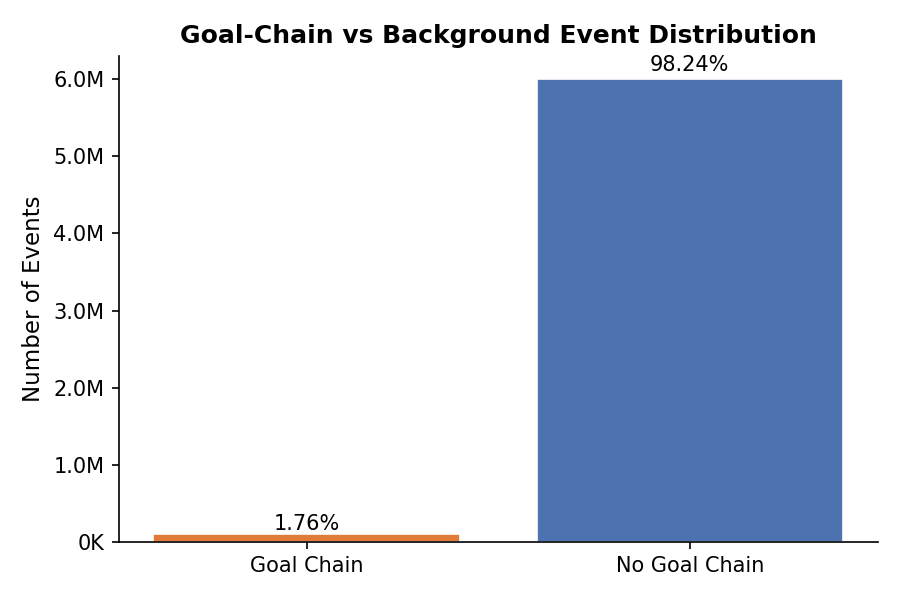
\includegraphics[width=0.7\textwidth]{../figures/eda_class_balance.png}
    \caption{Distribution of goal-chain events versus background events in the Version 1 dataset. Only 1.76\% of events belong to a goal-scoring possession chain, reflecting the fundamental rarity of goals in football.}
    \label{fig:class_balance}
\end{figure}

\begin{figure}[h]
    \centering
    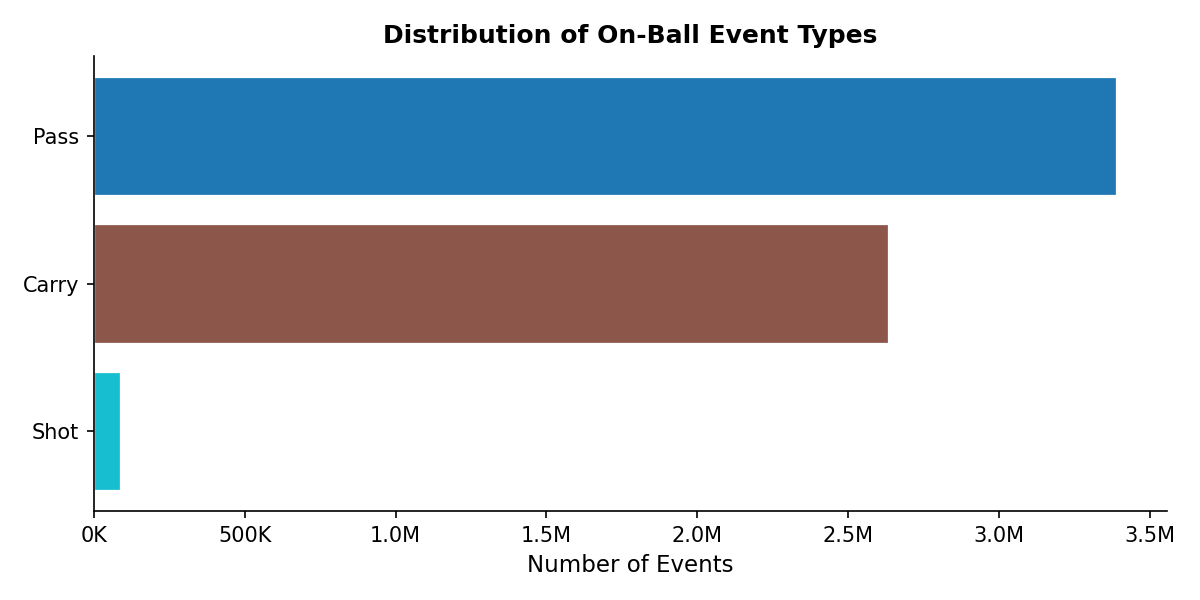
\includegraphics[width=0.85\textwidth]{../figures/eda_event_types.png}
    \caption{Distribution of on-ball event types in the Version 1 dataset. Passes account for the largest share, with shots constituting a small fraction of total events.}
    \label{fig:event_types}
\end{figure}

\begin{figure}[h]
    \centering
    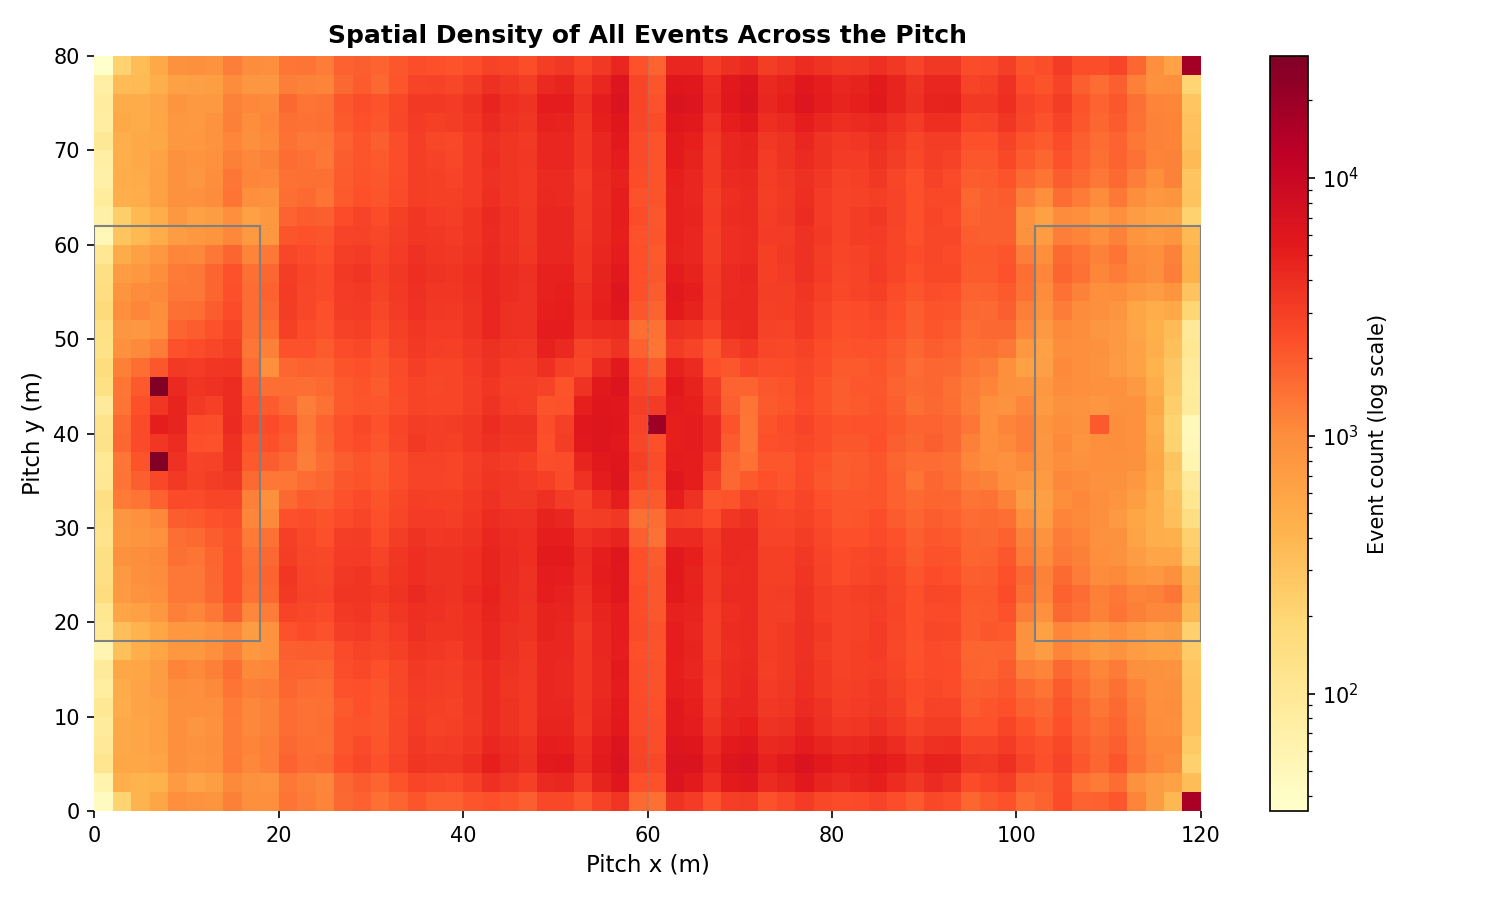
\includegraphics[width=0.85\textwidth]{../figures/eda_spatial_density.png}
    \caption{Spatial density of all events across the pitch (Version 1 dataset). Darker regions indicate higher event frequency. Activity is concentrated in central areas with a secondary cluster around the attacking penalty area.}
    \label{fig:spatial_density}
\end{figure}

\begin{figure}[h]
    \centering
    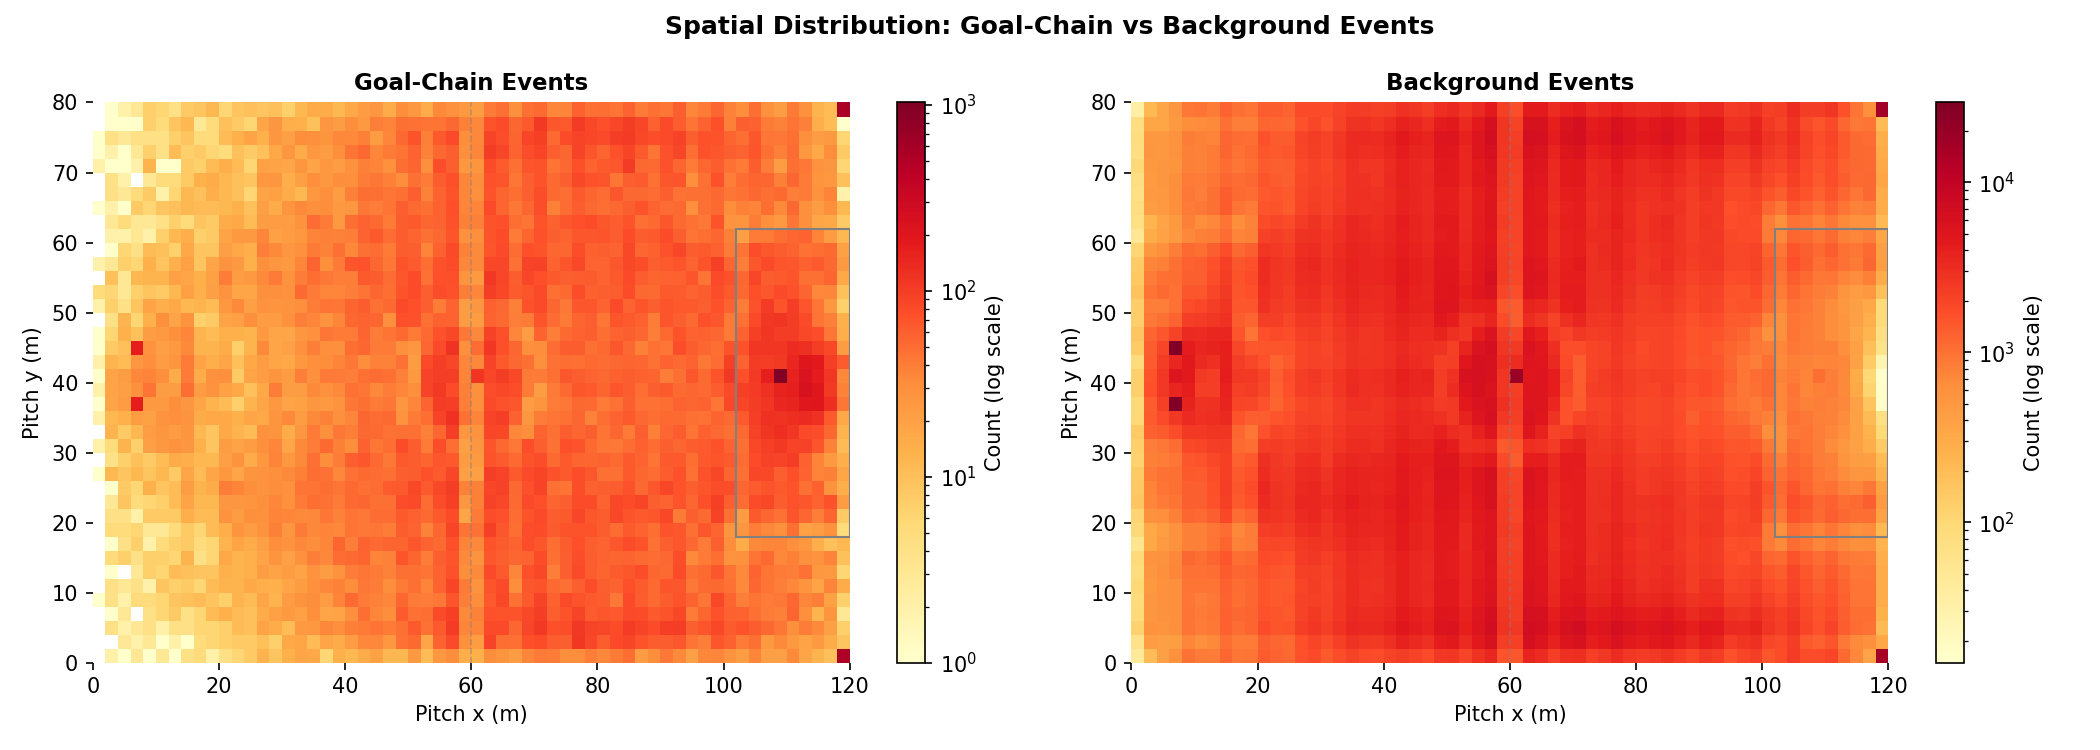
\includegraphics[width=0.85\textwidth]{../figures/eda_goal_chain_locs.png}
    \caption{Spatial distribution of goal-chain events (left) versus background events (right). Goal-chain events are strongly concentrated near the attacking goal, confirming that distance to goal is the primary predictor of threat.}
    \label{fig:goal_chain_locs}
\end{figure}

\begin{figure}[h]
    \centering
    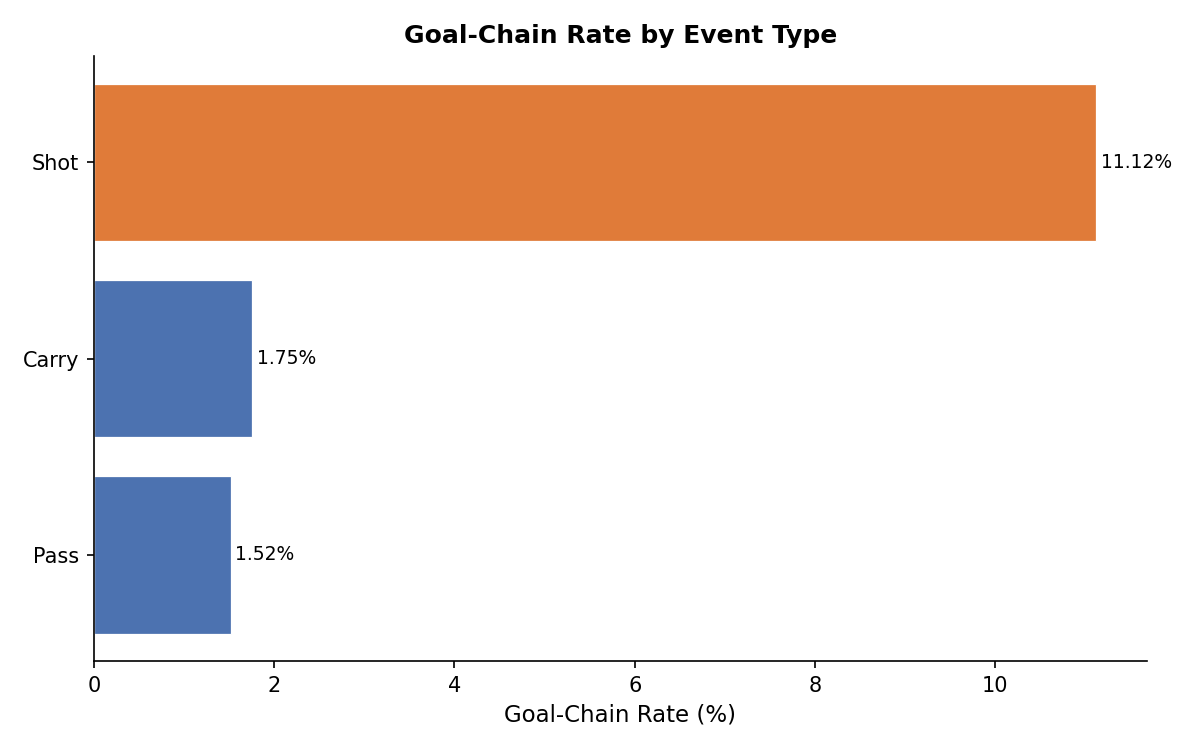
\includegraphics[width=0.8\textwidth]{../figures/eda_goal_rate_by_type.png}
    \caption{Goal-chain rate per event type. Shots dominate; and carries show the highest rates among non-shot actions.}
    \label{fig:goal_rate_type}
\end{figure}

\begin{figure}[h]
    \centering
    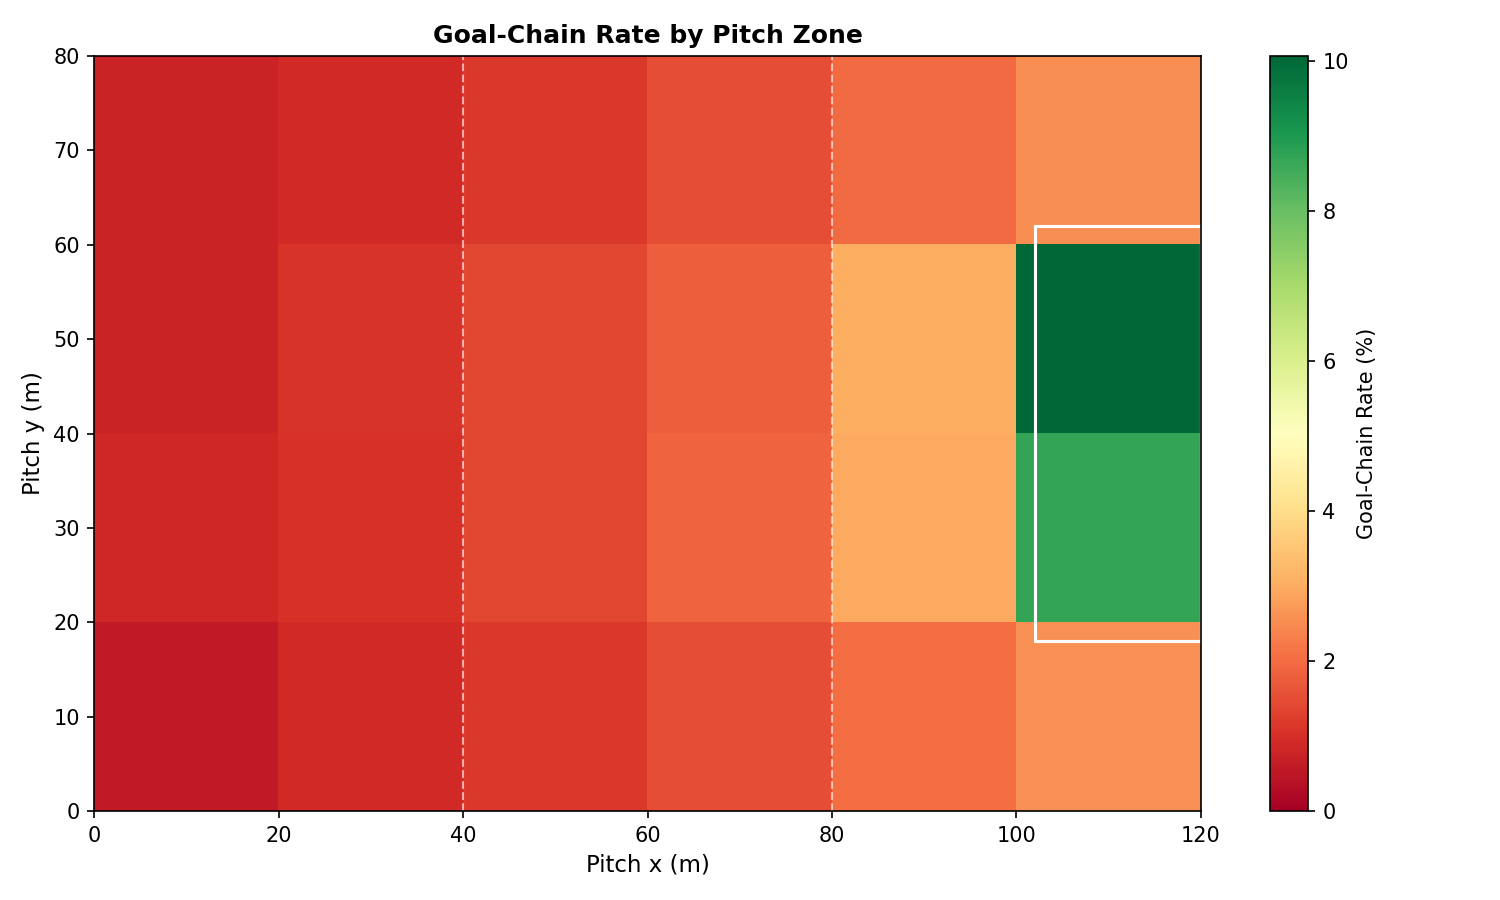
\includegraphics[width=0.85\textwidth]{../figures/eda_goal_rate_by_zone.png}
    \caption{Goal-chain rate by pitch zone. The attacking penalty area shows the highest rates, confirming spatial position as the dominant predictor of threat.}
    \label{fig:goal_rate_zone}
\end{figure}

\begin{figure}[h]
    \centering
    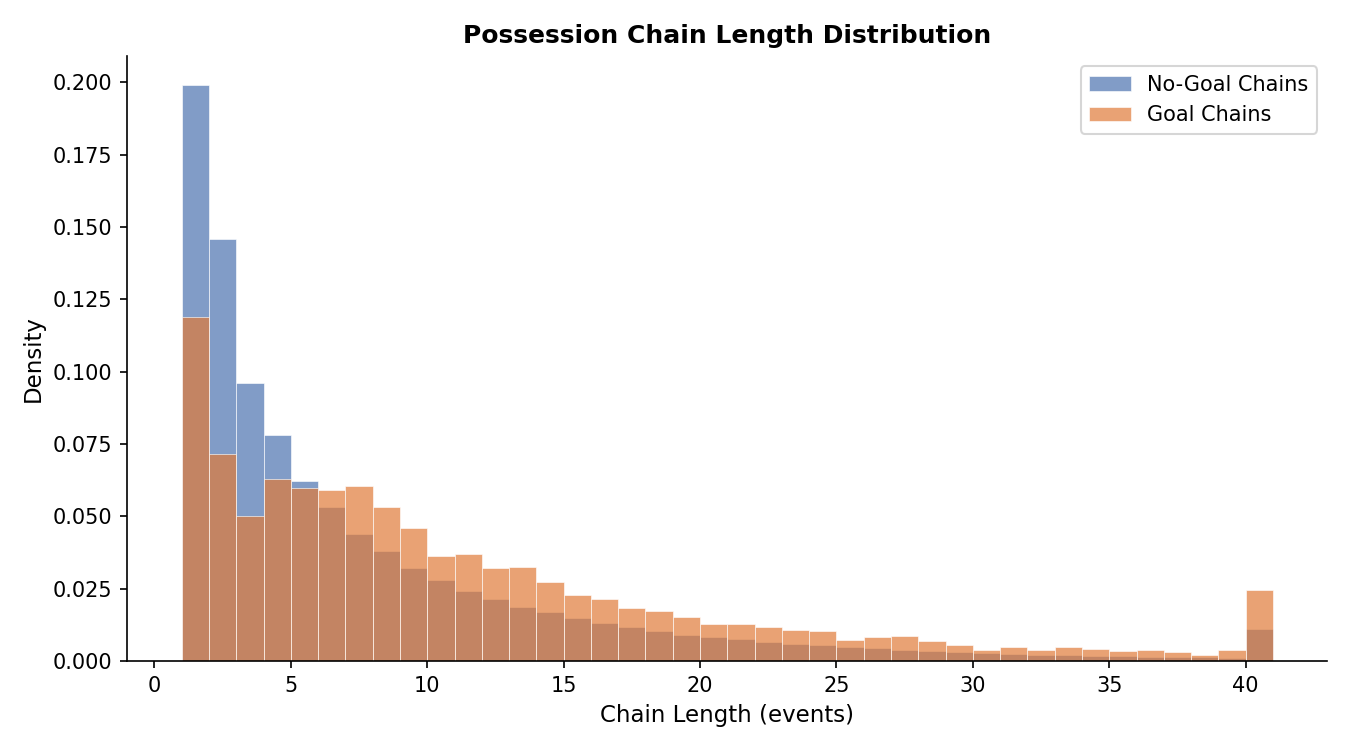
\includegraphics[width=0.8\textwidth]{../figures/eda_chain_lengths.png}
    \caption{Possession chain length distribution for goal-scoring and background chains. Goal chains are typically shorter and more direct.}
    \label{fig:chain_lengths}
\end{figure}

\begin{figure}[h]
    \centering
    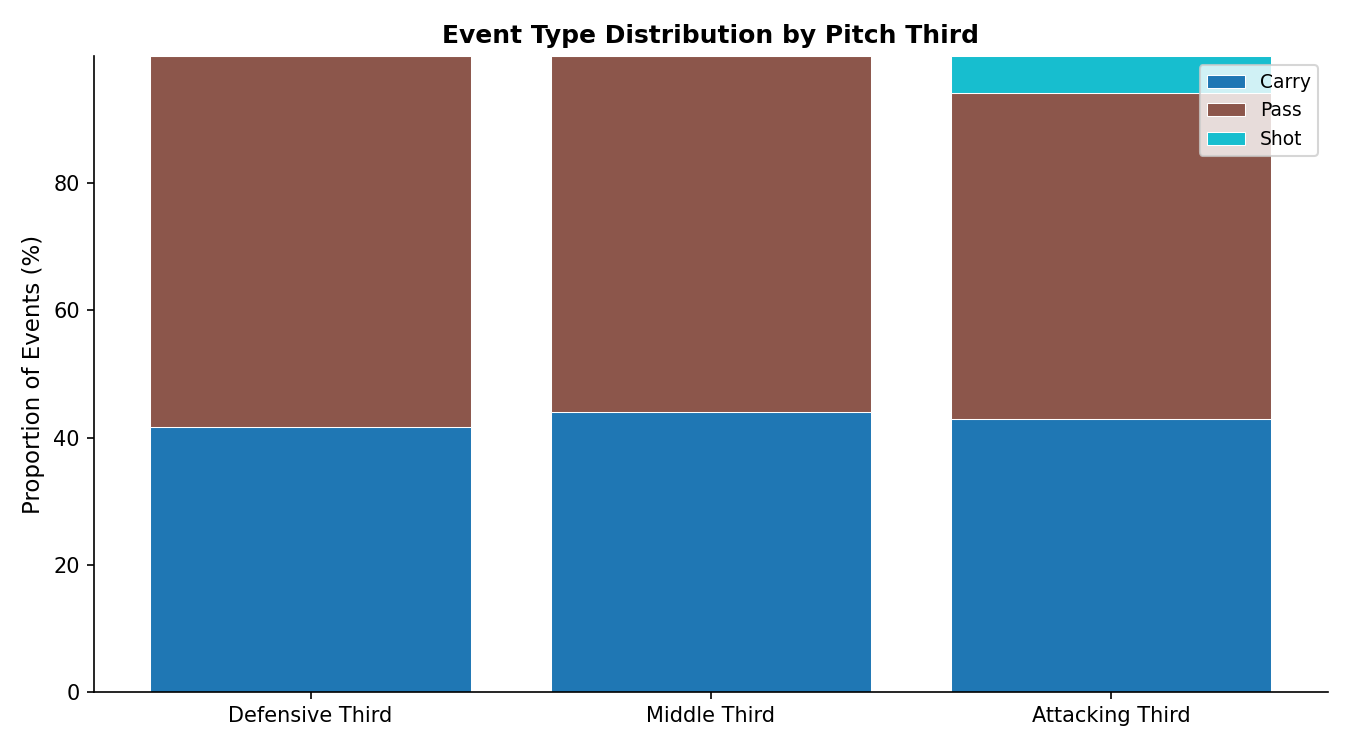
\includegraphics[width=0.85\textwidth]{../figures/eda_action_by_third.png}
    \caption{Proportion of each event type within the defensive, middle, and attacking thirds.}
    \label{fig:action_by_third}
\end{figure}

\begin{figure}[h]
    \centering
    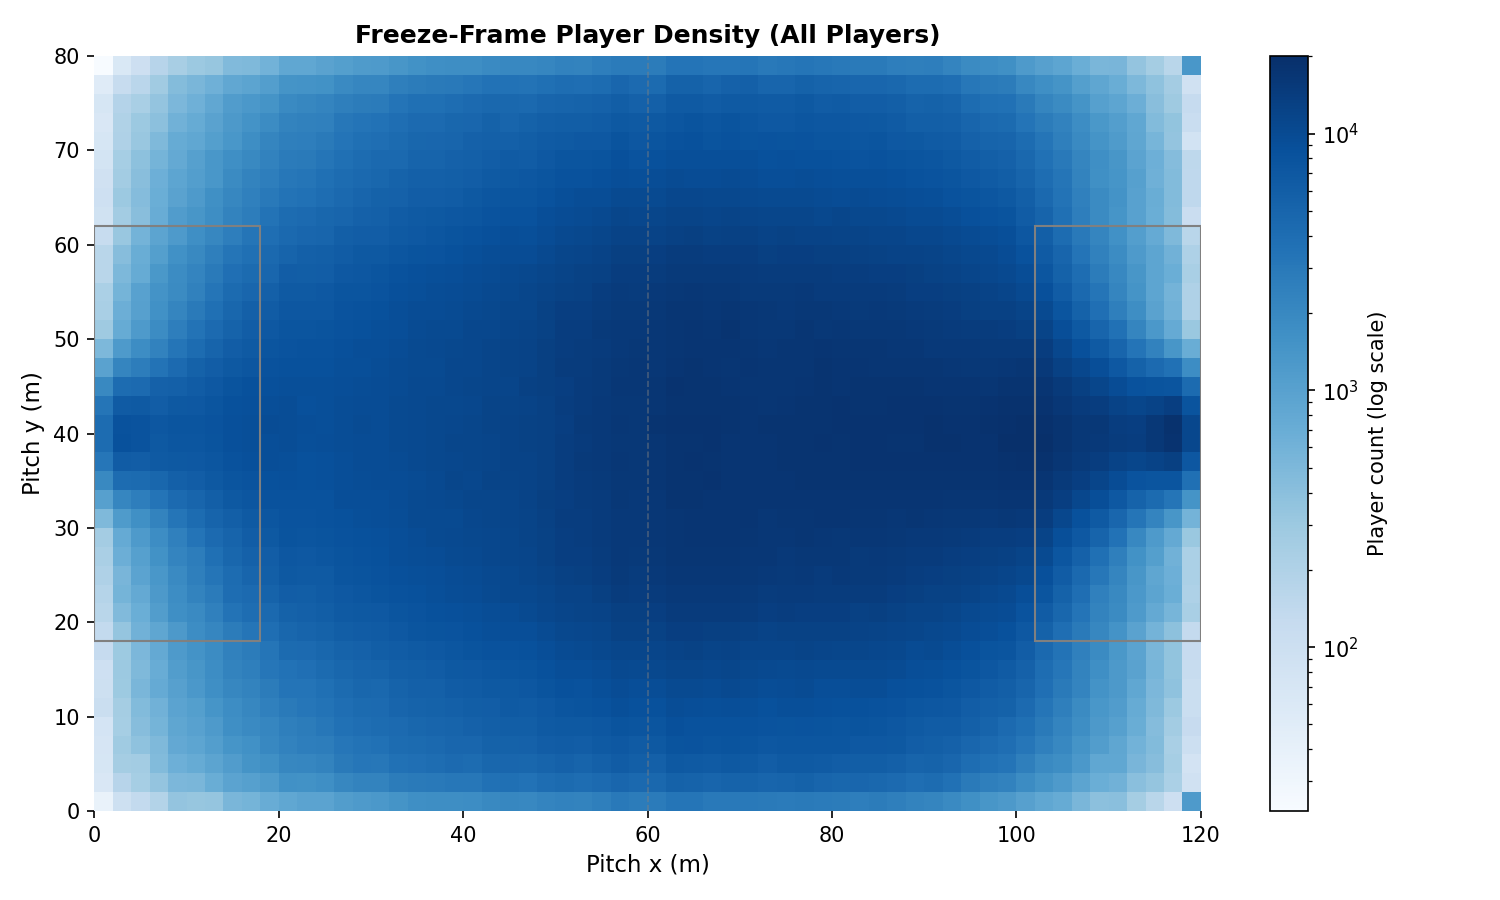
\includegraphics[width=0.85\textwidth]{../figures/eda_player_density.png}
    \caption{Spatial density of all player positions in 360 freeze frames (log scale). Players concentrate around the ball and in central corridors.}
    \label{fig:player_density}
\end{figure}

\begin{figure}[h]
    \centering
    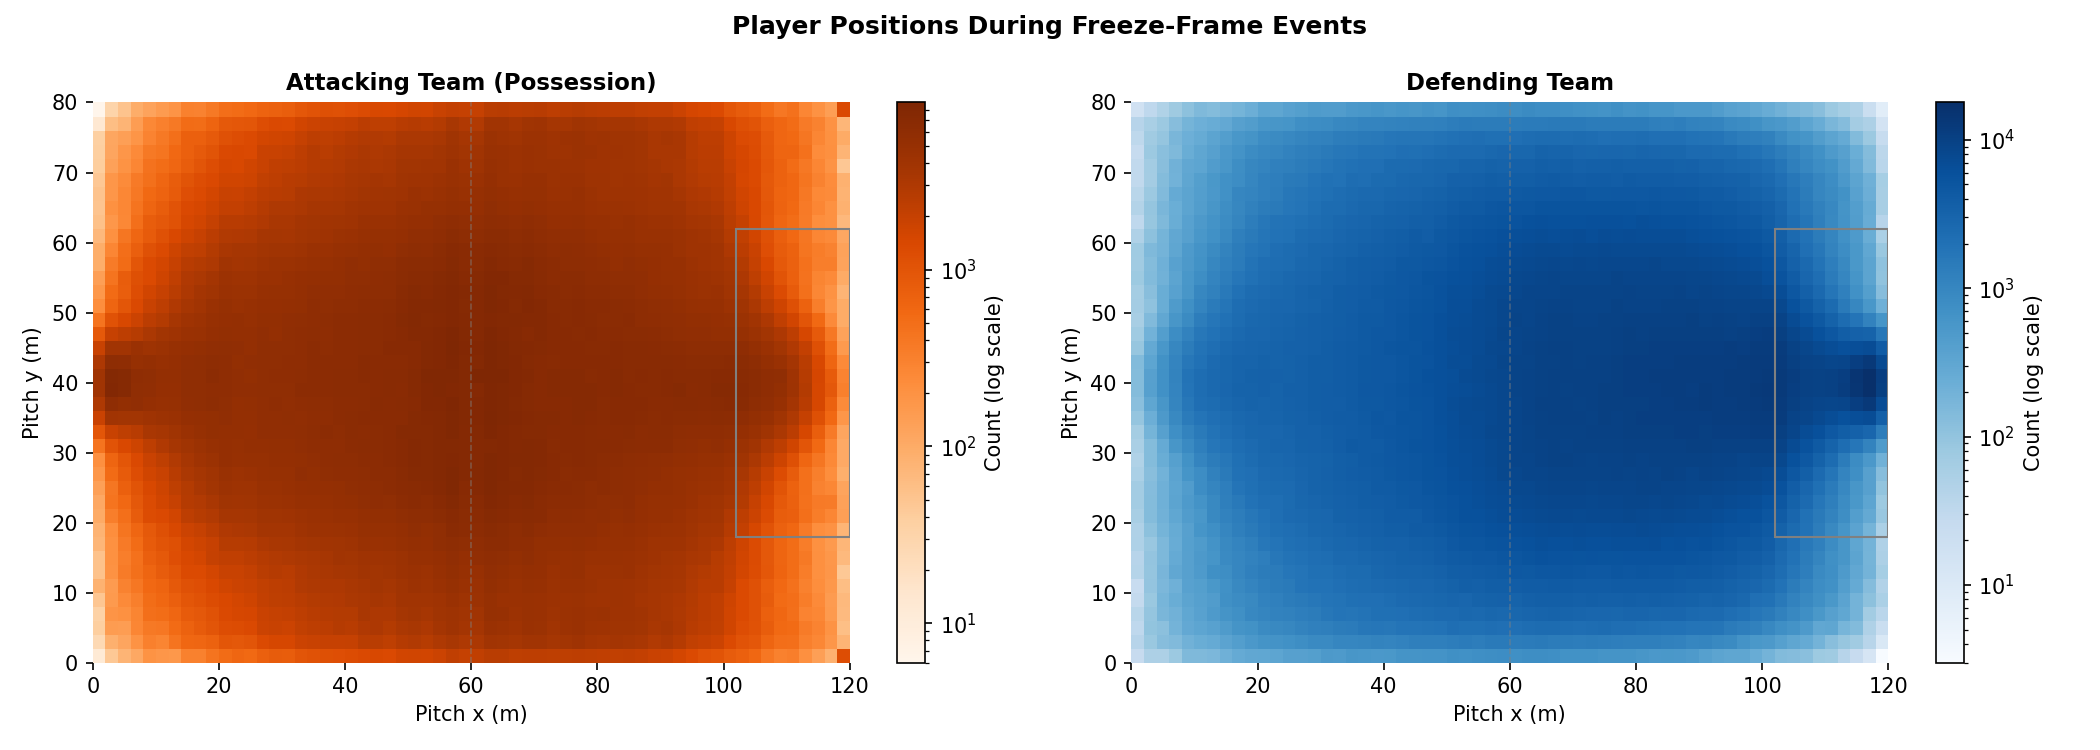
\includegraphics[width=\textwidth]{../figures/eda_team_positions.png}
    \caption{Freeze-frame player positions split by attacking team (left) and defending team (right). The teams occupy clearly distinct regions of the pitch.}
    \label{fig:team_positions}
\end{figure}

\begin{figure}[h]
    \centering
    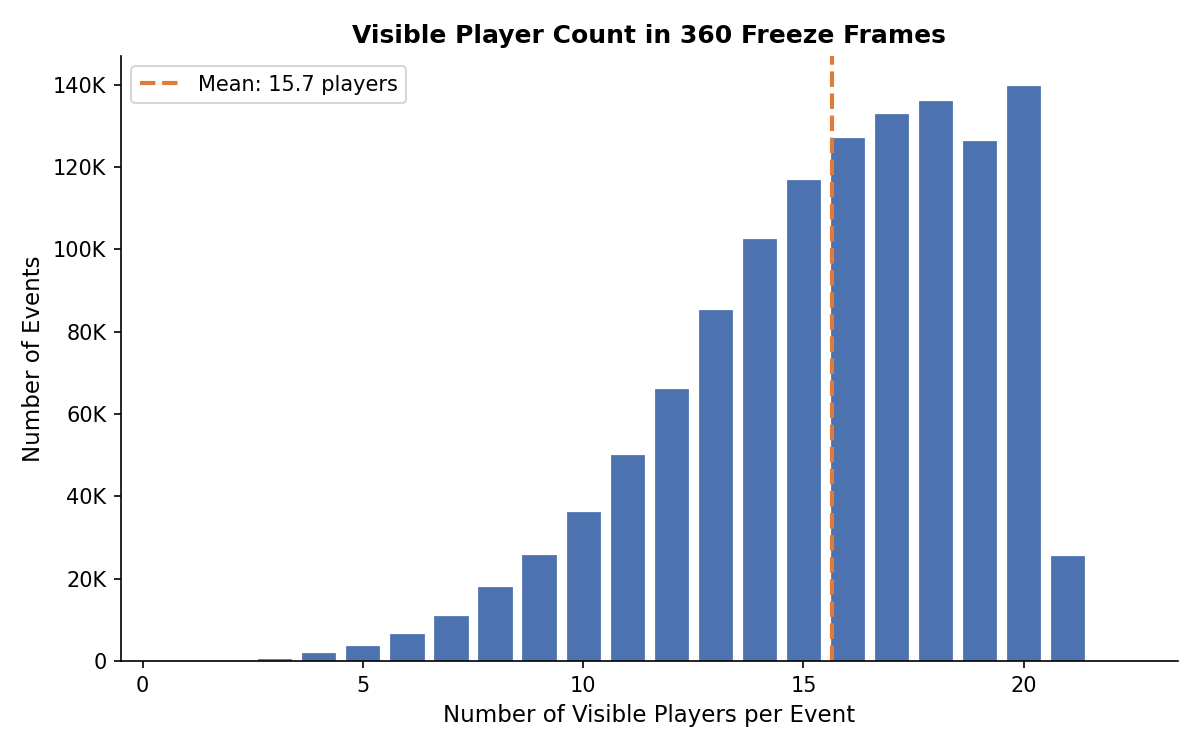
\includegraphics[width=0.7\textwidth]{../figures/eda_player_count.png}
    \caption{Distribution of visible player counts per freeze-frame event. Most events capture near-complete player information, validating the 360 data as a reliable source of positional context.}
    \label{fig:player_count}
\end{figure}

\clearpage

\section{Feature Correlation}

\begin{figure}[h]
    \centering
    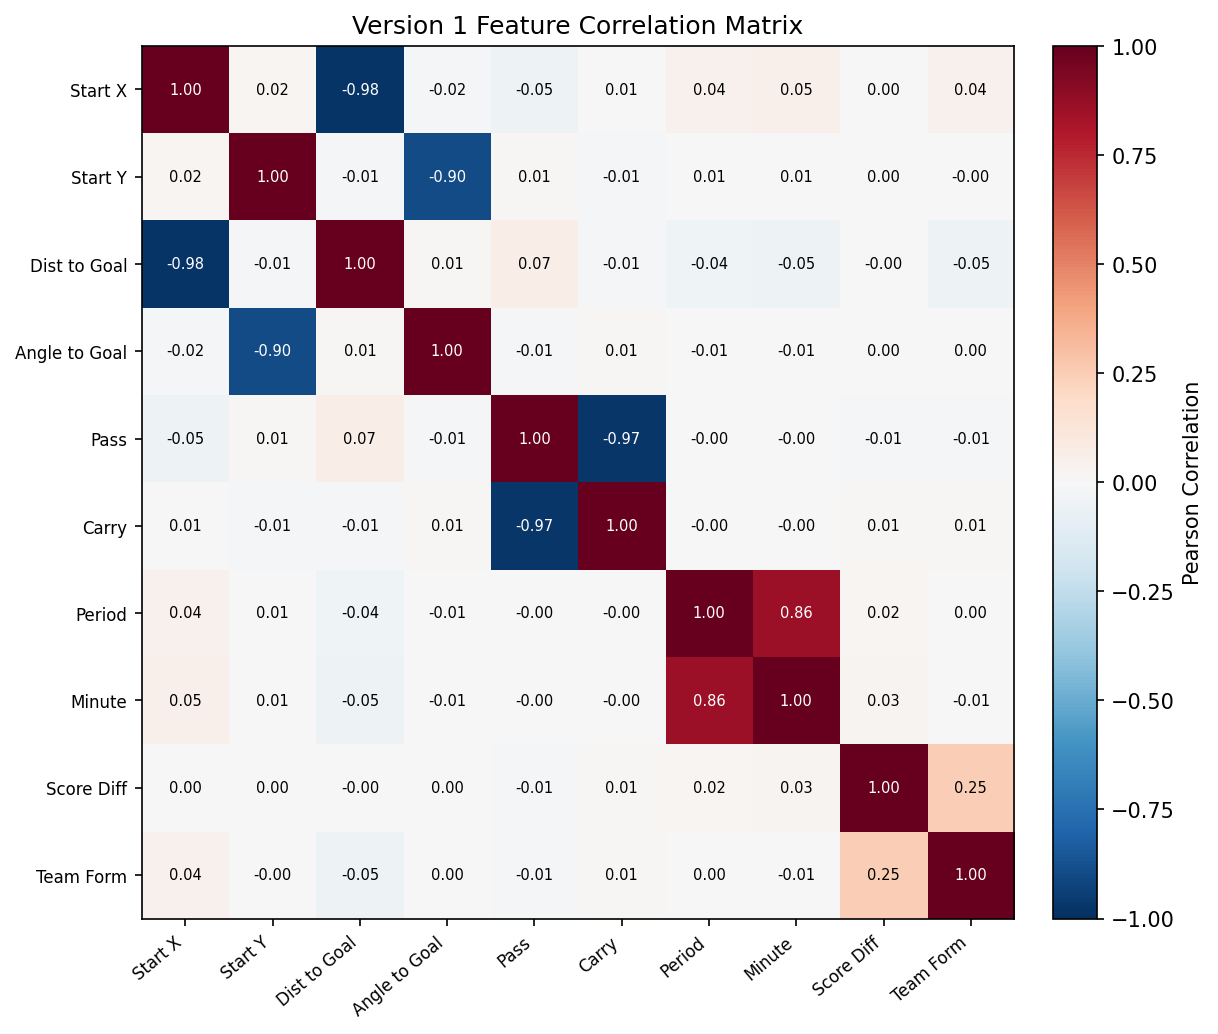
\includegraphics[width=0.72\textwidth]{../xT_v1/xt_feature_correlation.png}
    \caption{Pearson correlation matrix for Version 1 input features.}
    \label{fig:feat_corr}
\end{figure}

\clearpage

\section{Version 1: Random Forest}

\begin{figure}[h]
    \centering
    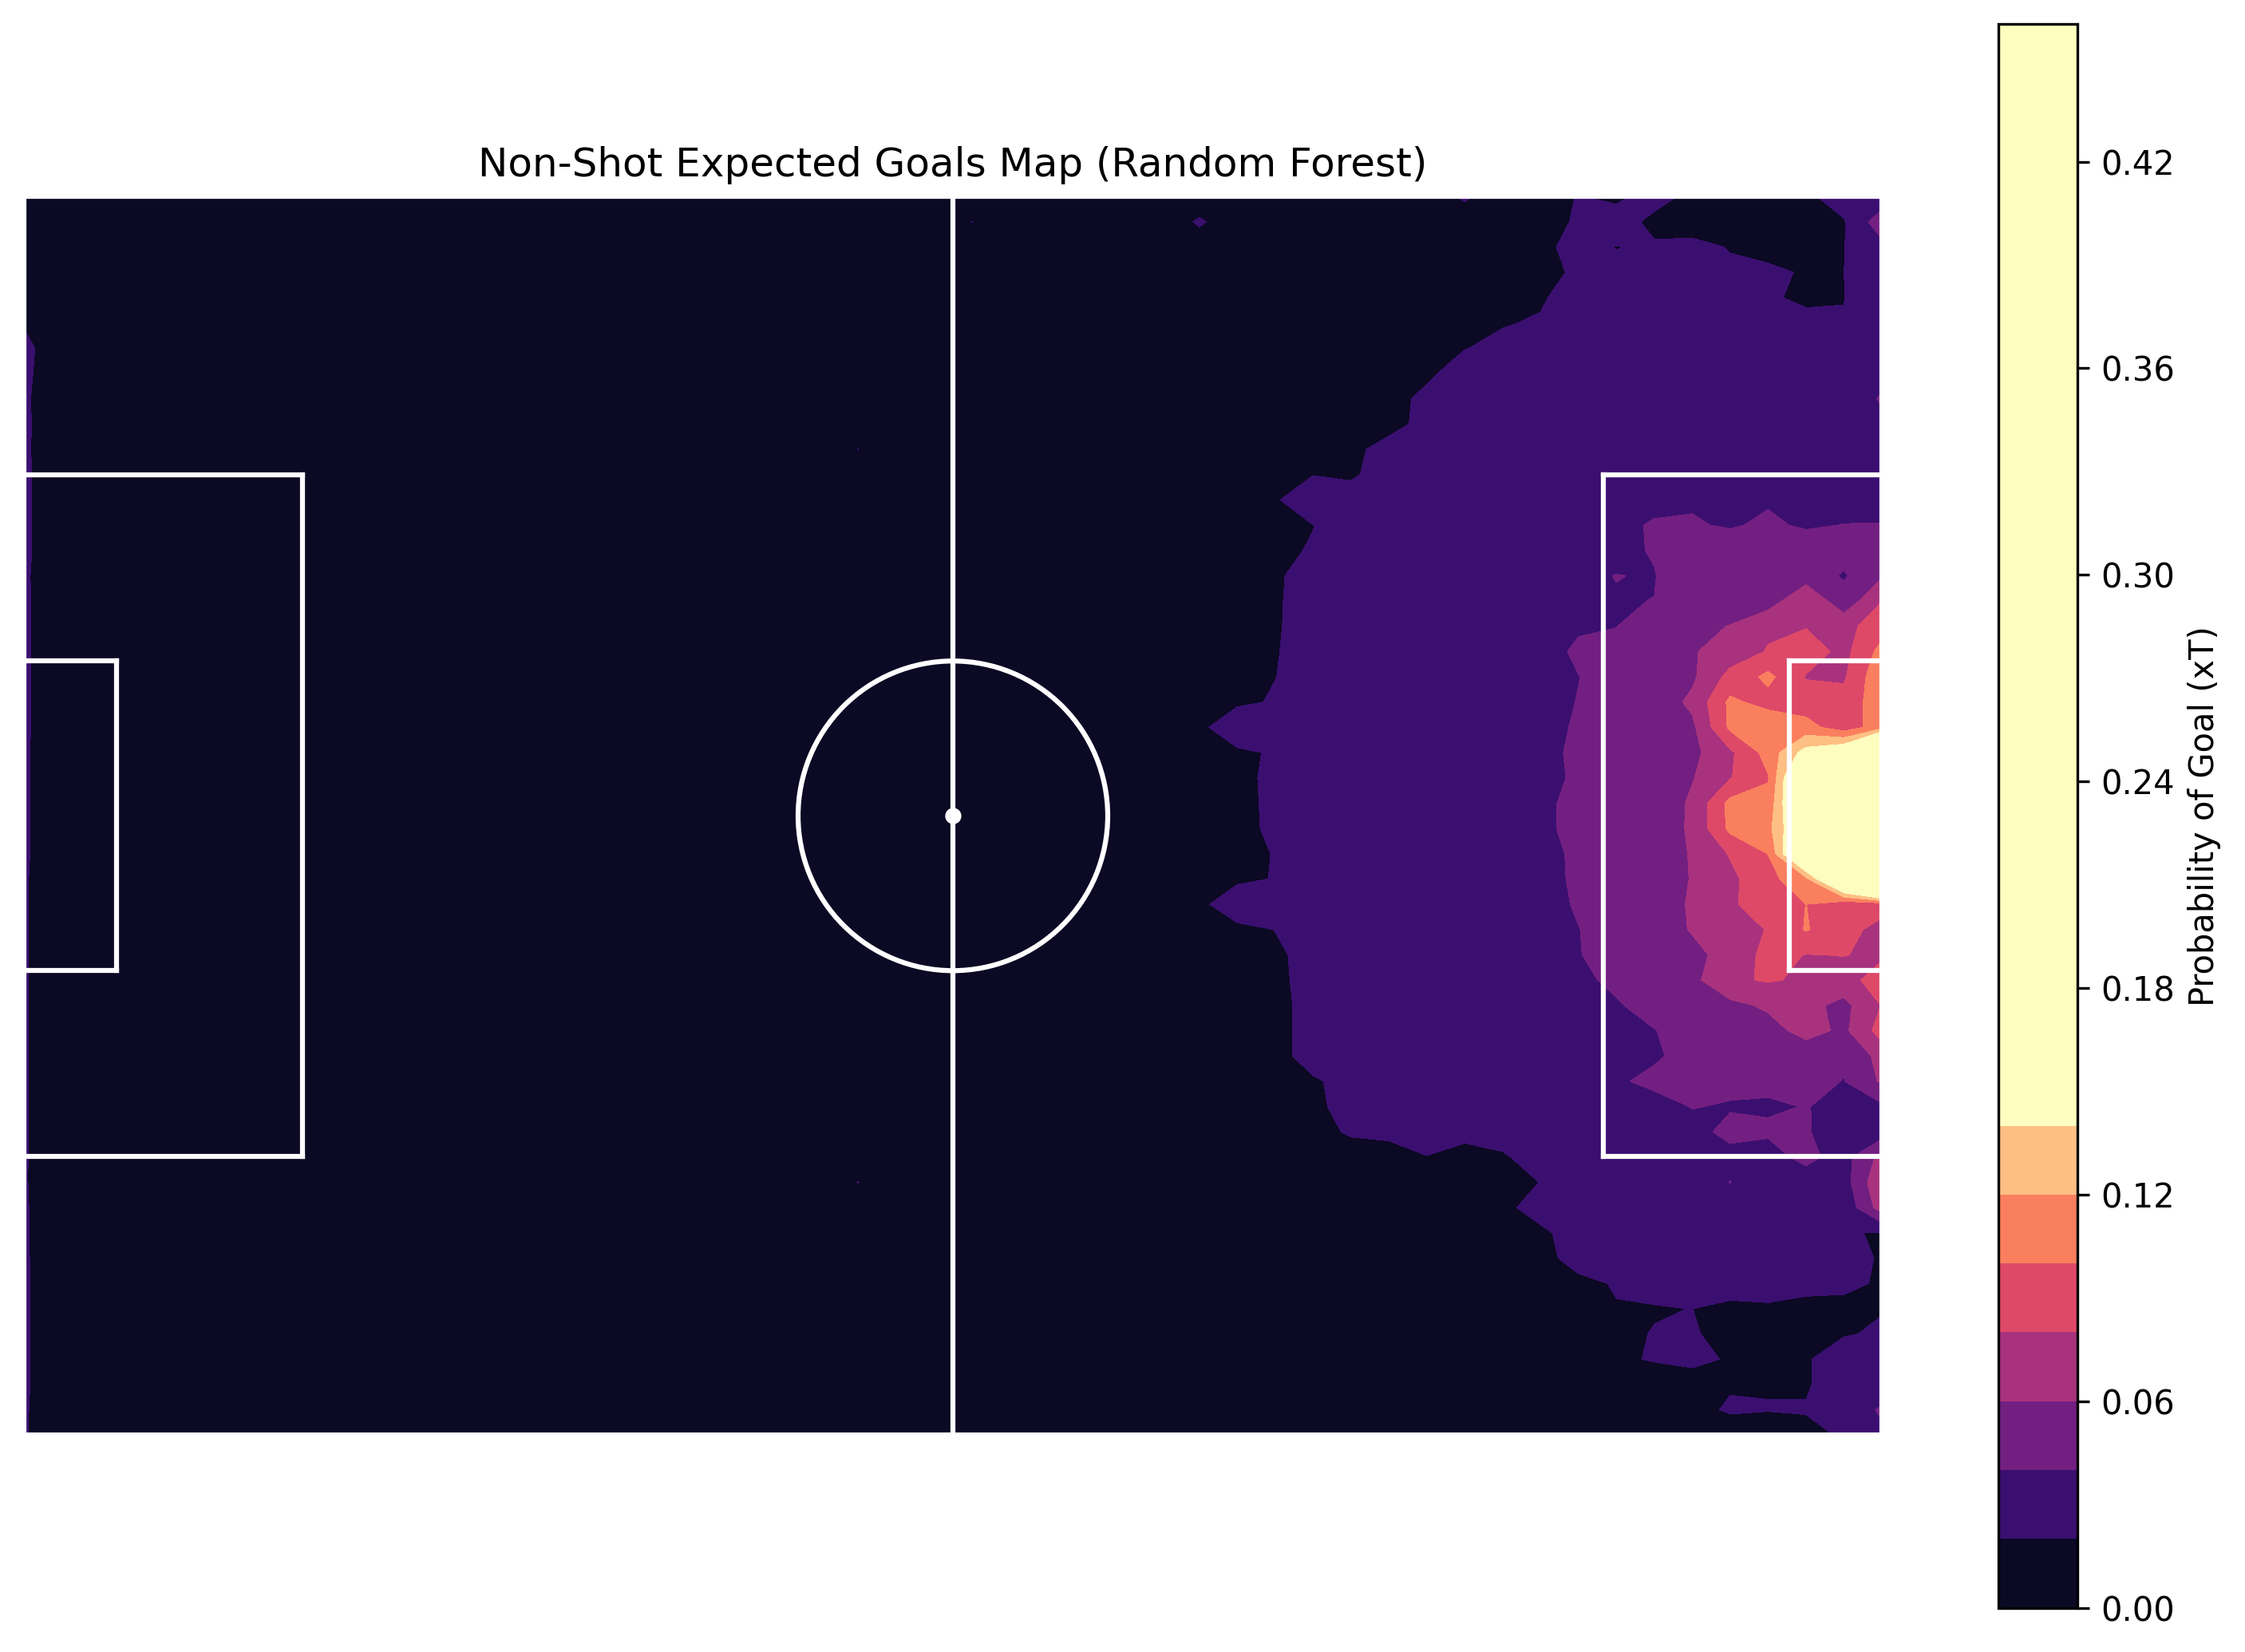
\includegraphics[width=0.8\textwidth]{../xT_v1/xt_heatmap.png}
    \caption{SxT heatmap for Version 1 (Random Forest), generated by querying the model at every grid cell assuming a Pass action type at a neutral game state (period 2, minute 45, score level, average team form). See Appendix~\ref{app:metrics} for full metric tables.}
    \label{fig:v1_heatmap}
\end{figure}

\begin{figure}[h]
    \centering
    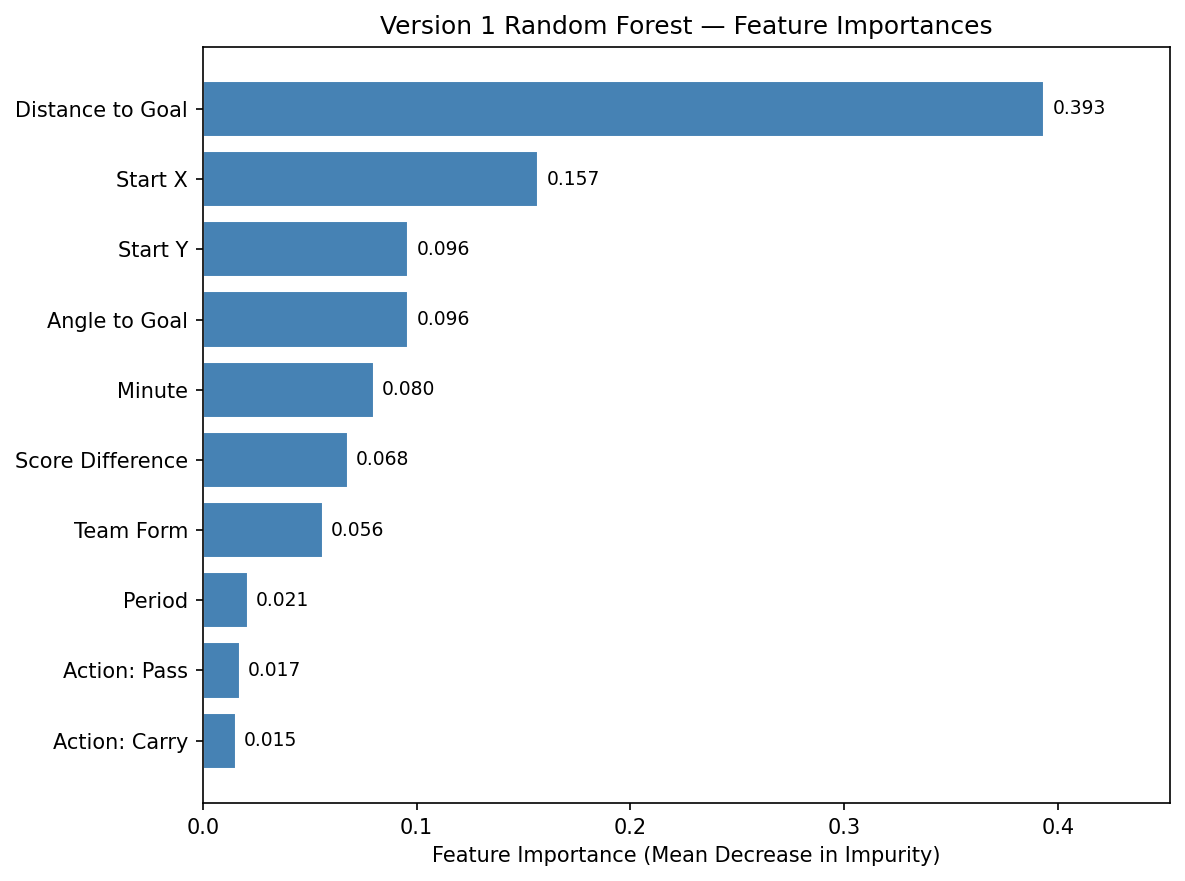
\includegraphics[width=0.85\textwidth]{../xT_v1/xt_feature_importance.png}
    \caption{Feature importance scores for the Version 1 Random Forest (mean decrease in impurity).}
    \label{fig:v1_importance}
\end{figure}

\clearpage

\section{Version 2: CNN + MLP}

\begin{figure}[h]
\centering
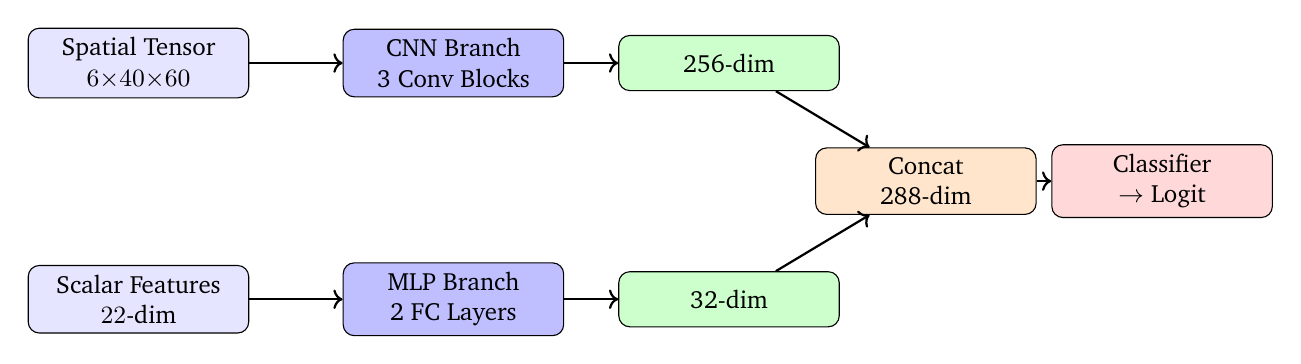
\begin{tikzpicture}[
    box/.style={draw, rounded corners, minimum width=2.8cm, minimum height=0.7cm, align=center, font=\small},
    arr/.style={->, thick}
]
\node[box, fill=blue!10]  (spatial) at (0, 3)    {Spatial Tensor\\$6{\times}40{\times}60$};
\node[box, fill=blue!10]  (scalar)  at (0, 0)    {Scalar Features\\$22$-dim};
\node[box, fill=blue!25]  (cnn)     at (4, 3)    {CNN Branch\\3 Conv Blocks};
\node[box, fill=blue!25]  (mlp)     at (4, 0)    {MLP Branch\\2 FC Layers};
\node[box, fill=green!20] (cnnout)  at (7.5, 3)  {256-dim};
\node[box, fill=green!20] (mlpout)  at (7.5, 0)  {32-dim};
\node[box, fill=orange!20](concat)  at (10, 1.5) {Concat\\288-dim};
\node[box, fill=red!15]   (cls)     at (13, 1.5) {Classifier\\$\to$ Logit};

\draw[arr] (spatial) -- (cnn);
\draw[arr] (scalar)  -- (mlp);
\draw[arr] (cnn)     -- (cnnout);
\draw[arr] (mlp)     -- (mlpout);
\draw[arr] (cnnout)  -- (concat);
\draw[arr] (mlpout)  -- (concat);
\draw[arr] (concat)  -- (cls);
\end{tikzpicture}
\caption{Version 2 dual-branch architecture. The CNN branch processes the spatial pitch tensor; the MLP branch processes scalar context features. Their outputs are concatenated and passed to a final classifier.}
\label{fig:v2arch}
\end{figure}

\begin{figure}[h]
    \centering
    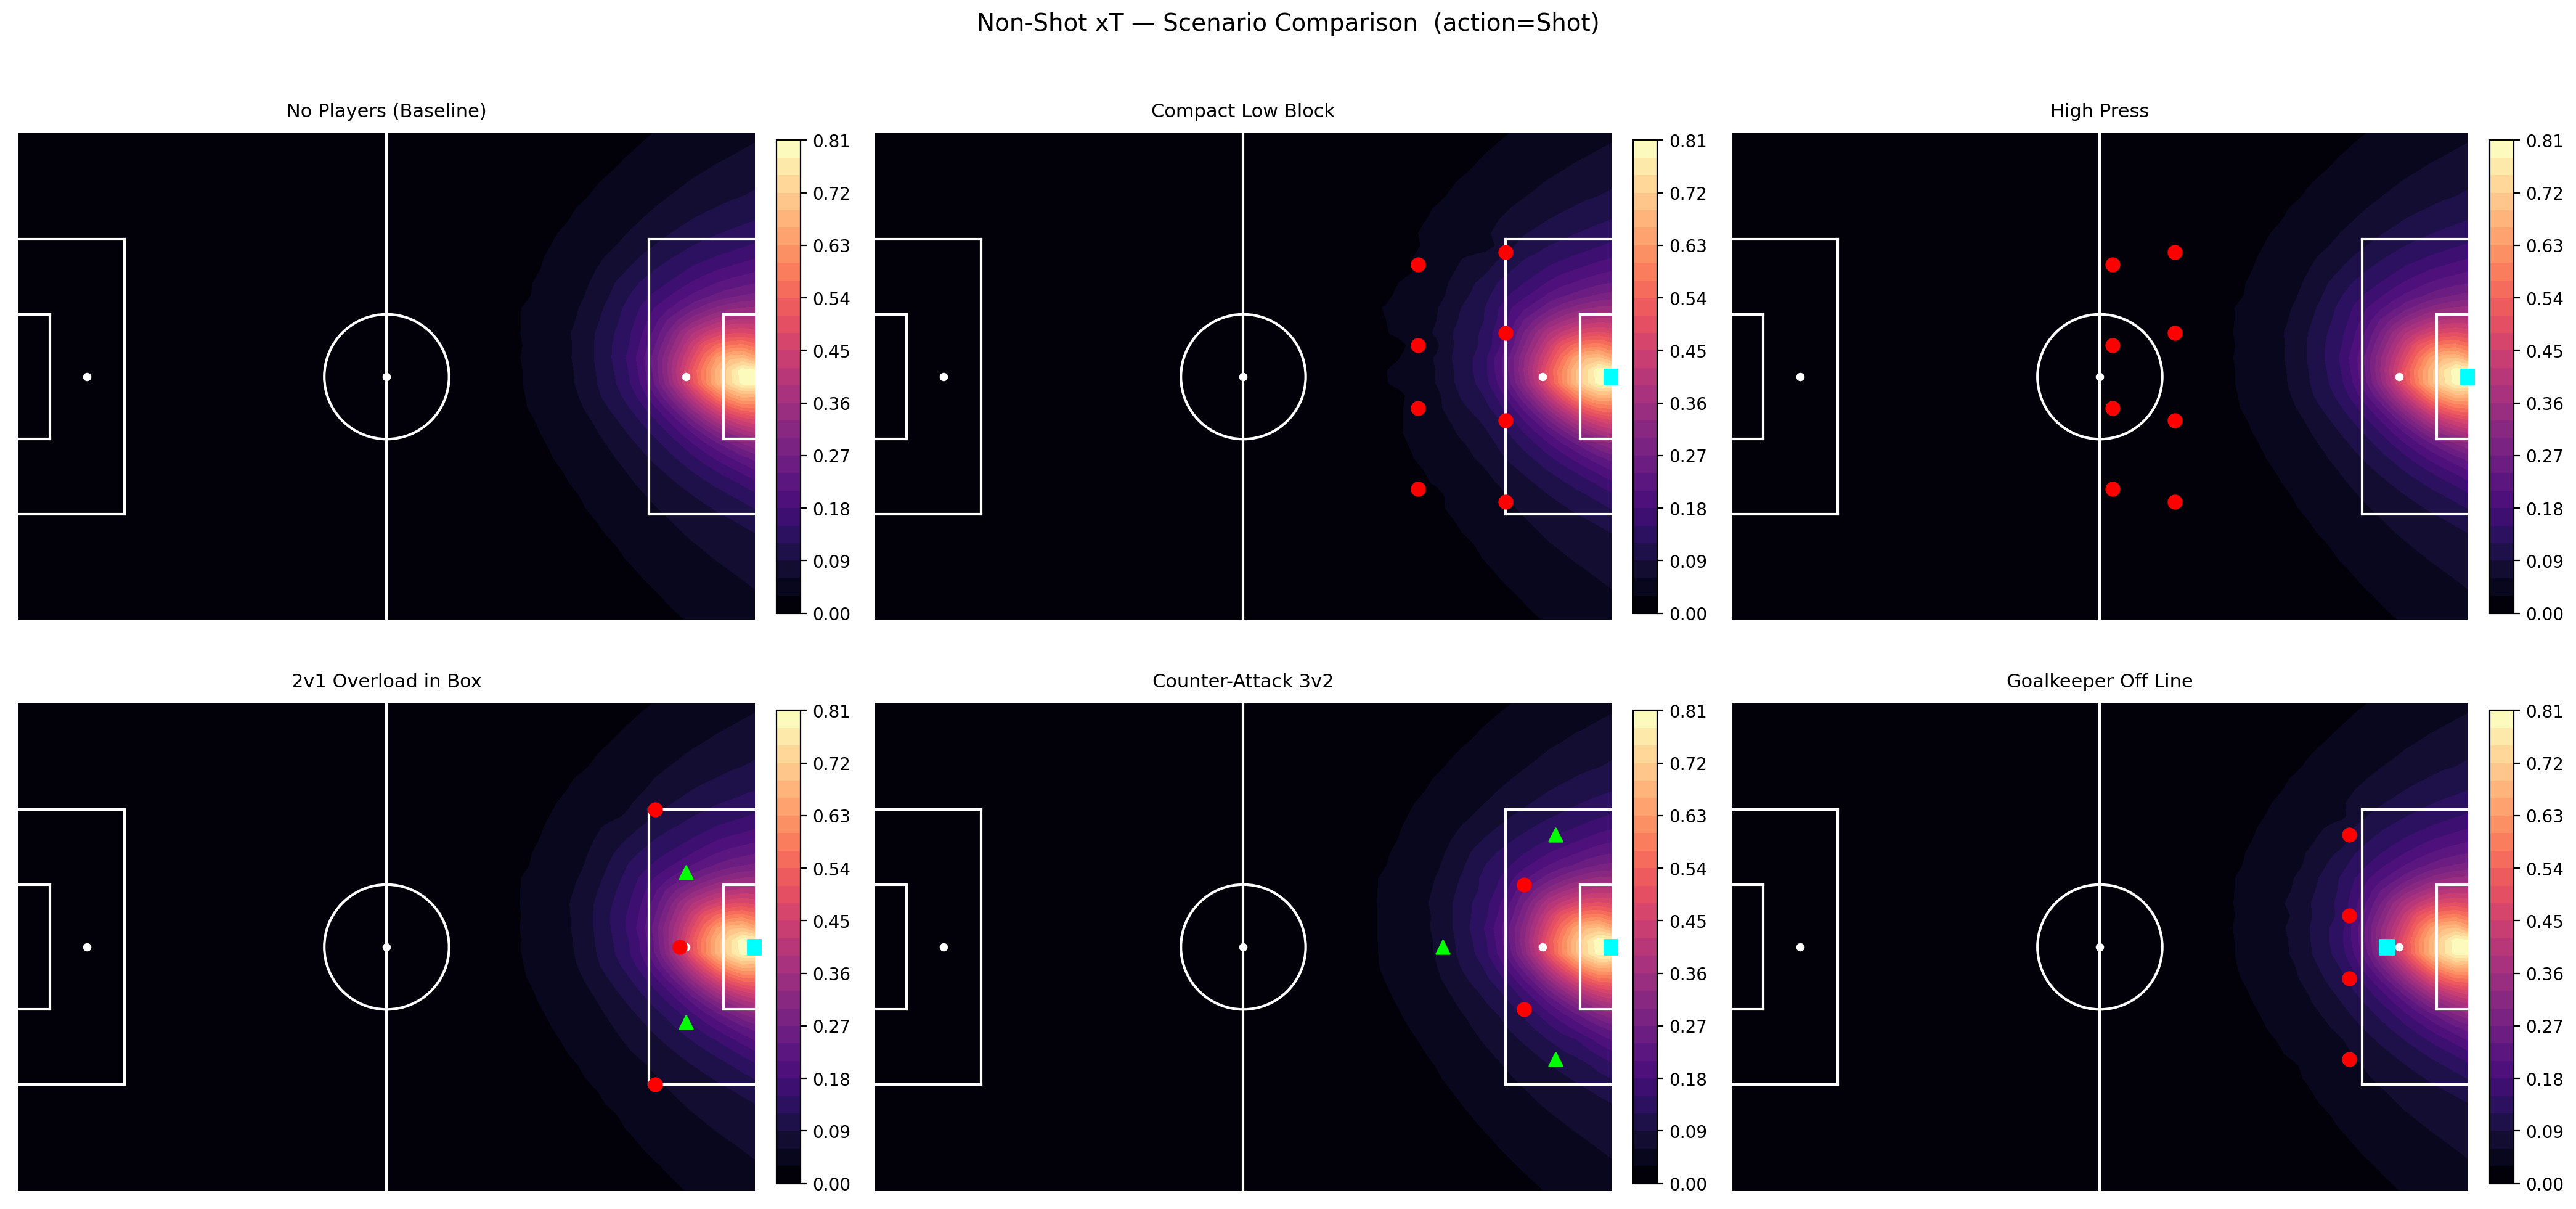
\includegraphics[width=0.8\textwidth]{../visualisations/xt_scenarios_shot_v2.png}
    \caption{Scenario comparison for Version 2, Shot action type. Six defensive configurations are shown under the same neutral game-state baseline (period 1, minute 0, score tied); the first panel (no players) serves as the positional reference. The near-identical surfaces across all panels illustrate the CNN's inability to distinguish between formations of equal density.}
    \label{fig:v2_scenarios}
\end{figure}

The following figures show Version 2 scenario grids for Pass, Carry, and Dribble. No standalone baseline heatmaps are shown; the \textit{No Players (Baseline)} panel in each grid already serves as the positional reference.

For Pass, the xT at each grid cell is computed by running the model once per outfield teammate in the scenario, using that teammate's position as the pass end-point, and taking the maximum xT over all targets. Panels without outfield teammates are shown as black (zero xT) by design: Pass xT is undefined without a specific target. Four of the six scenarios contain no teammates; only the 2v1 Overload and Counter-Attack panels show non-zero Pass threat. The same convention applies to the Version 3 grids in the following section.

\begin{figure}[h]
    \centering
    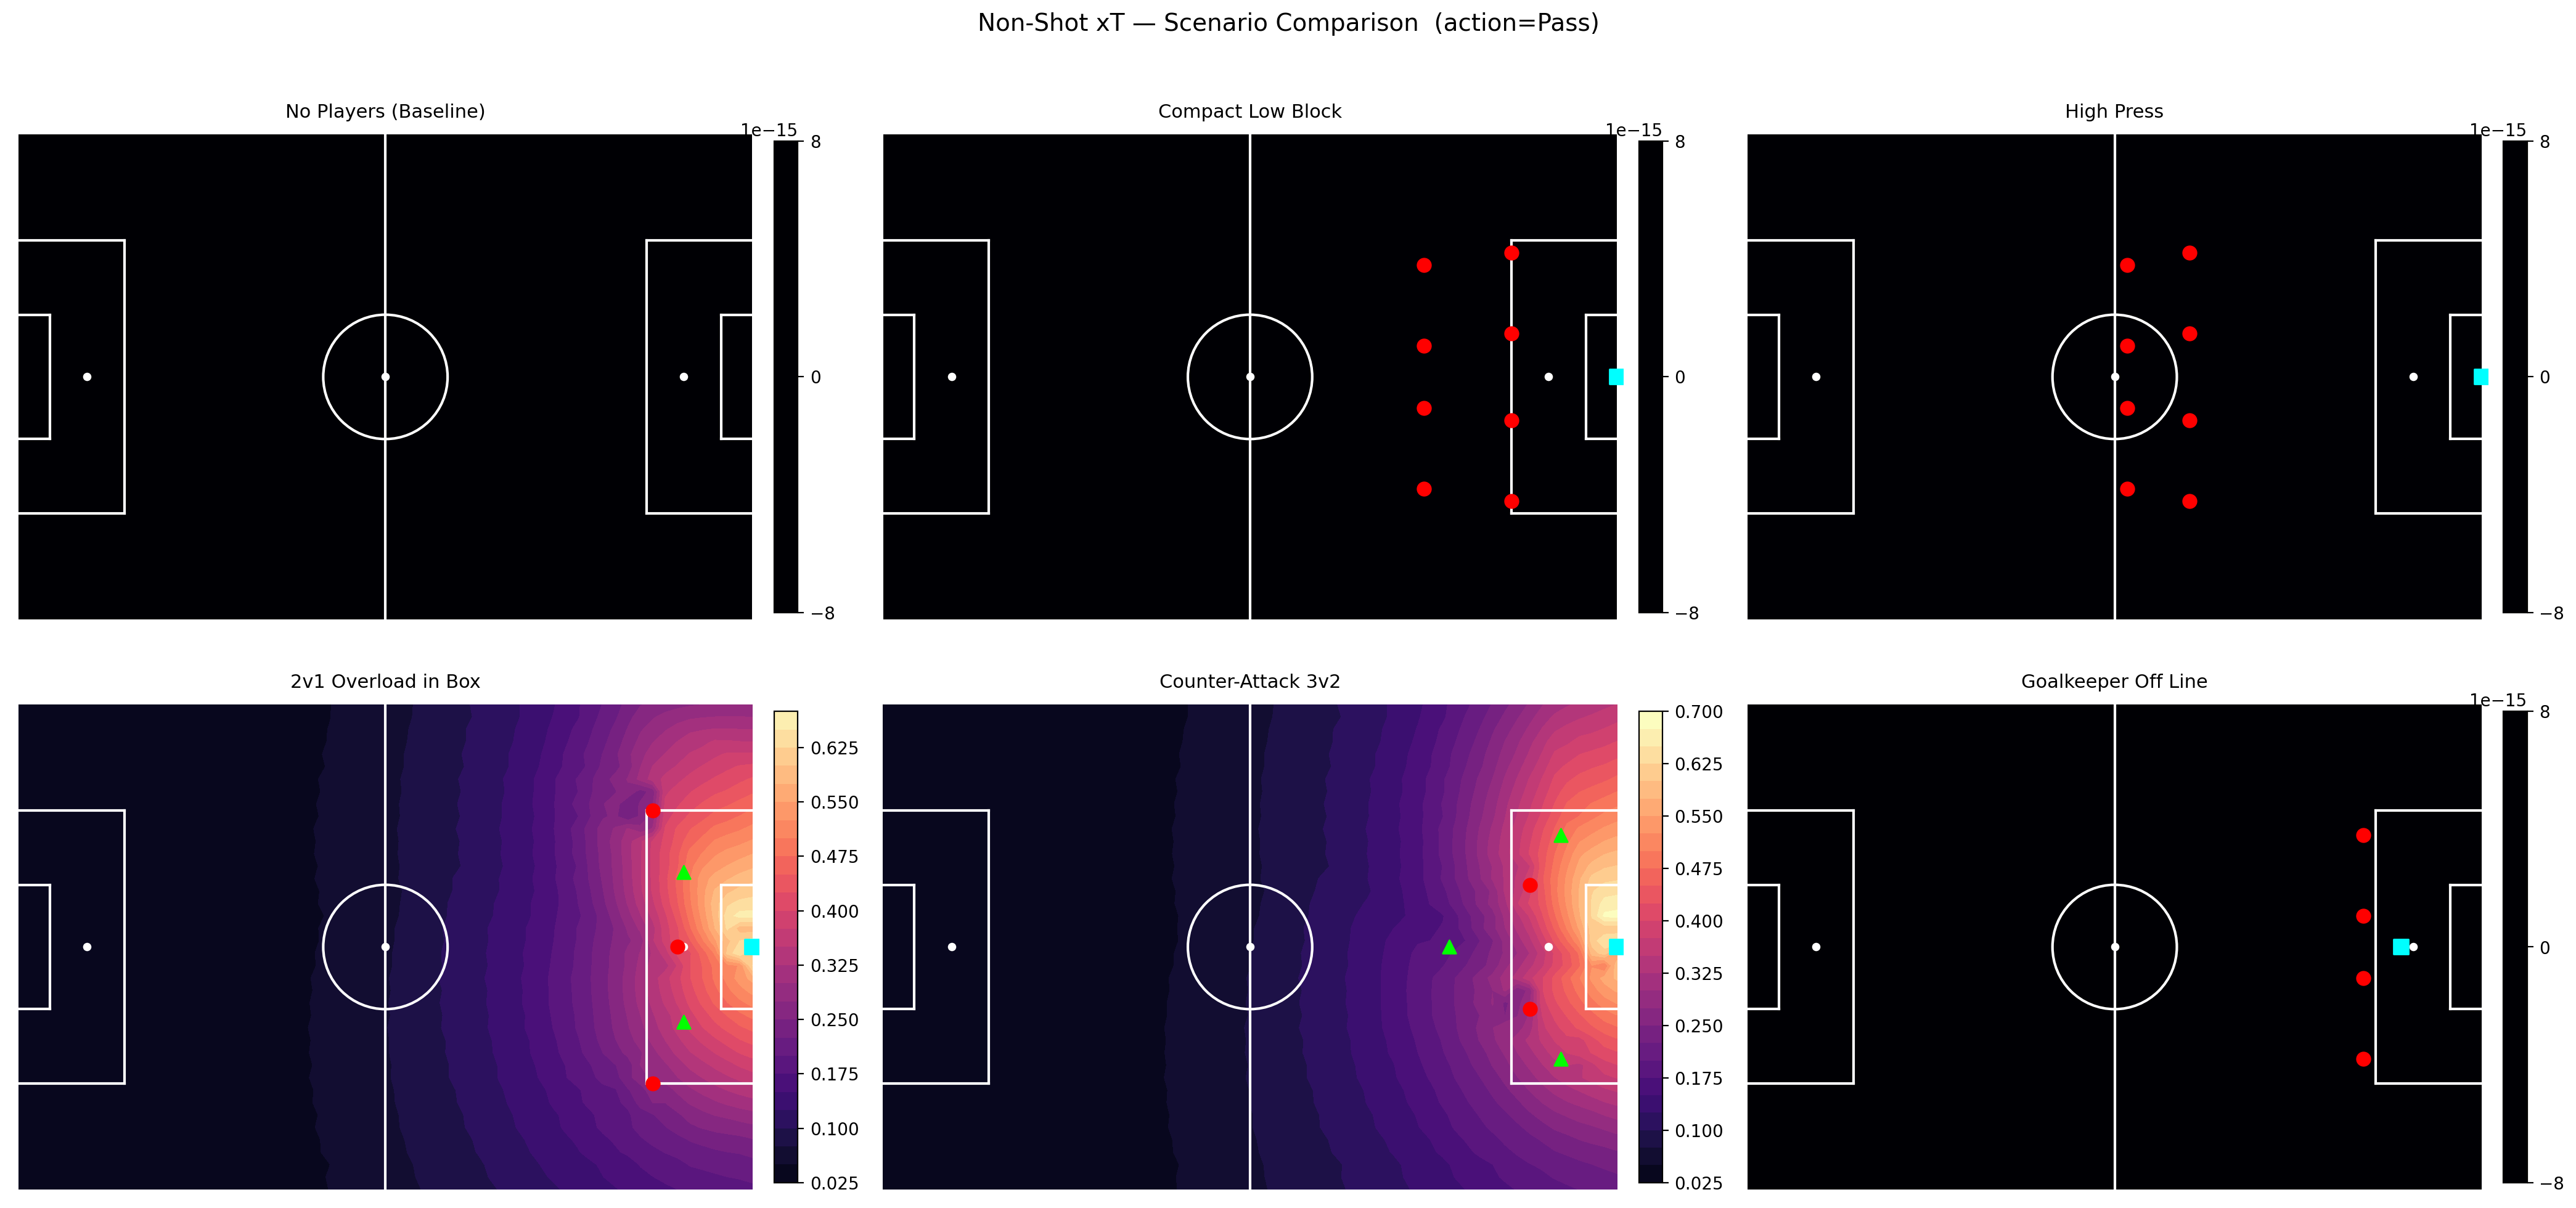
\includegraphics[width=0.8\textwidth]{../visualisations/xt_scenarios_pass_v2.png}
    \caption{Version 2 scenario comparison, Pass action type. Panels without outfield teammates are black --- Pass xT is zero when no target is available. The 2v1 Overload and Counter-Attack panels show non-zero threat reflecting passes to the positioned teammates. The CNN surfaces change little with formation, consistent with a density-based architecture.}
    \label{fig:v2_scenarios_pass}
\end{figure}

\begin{figure}[h]
    \centering
    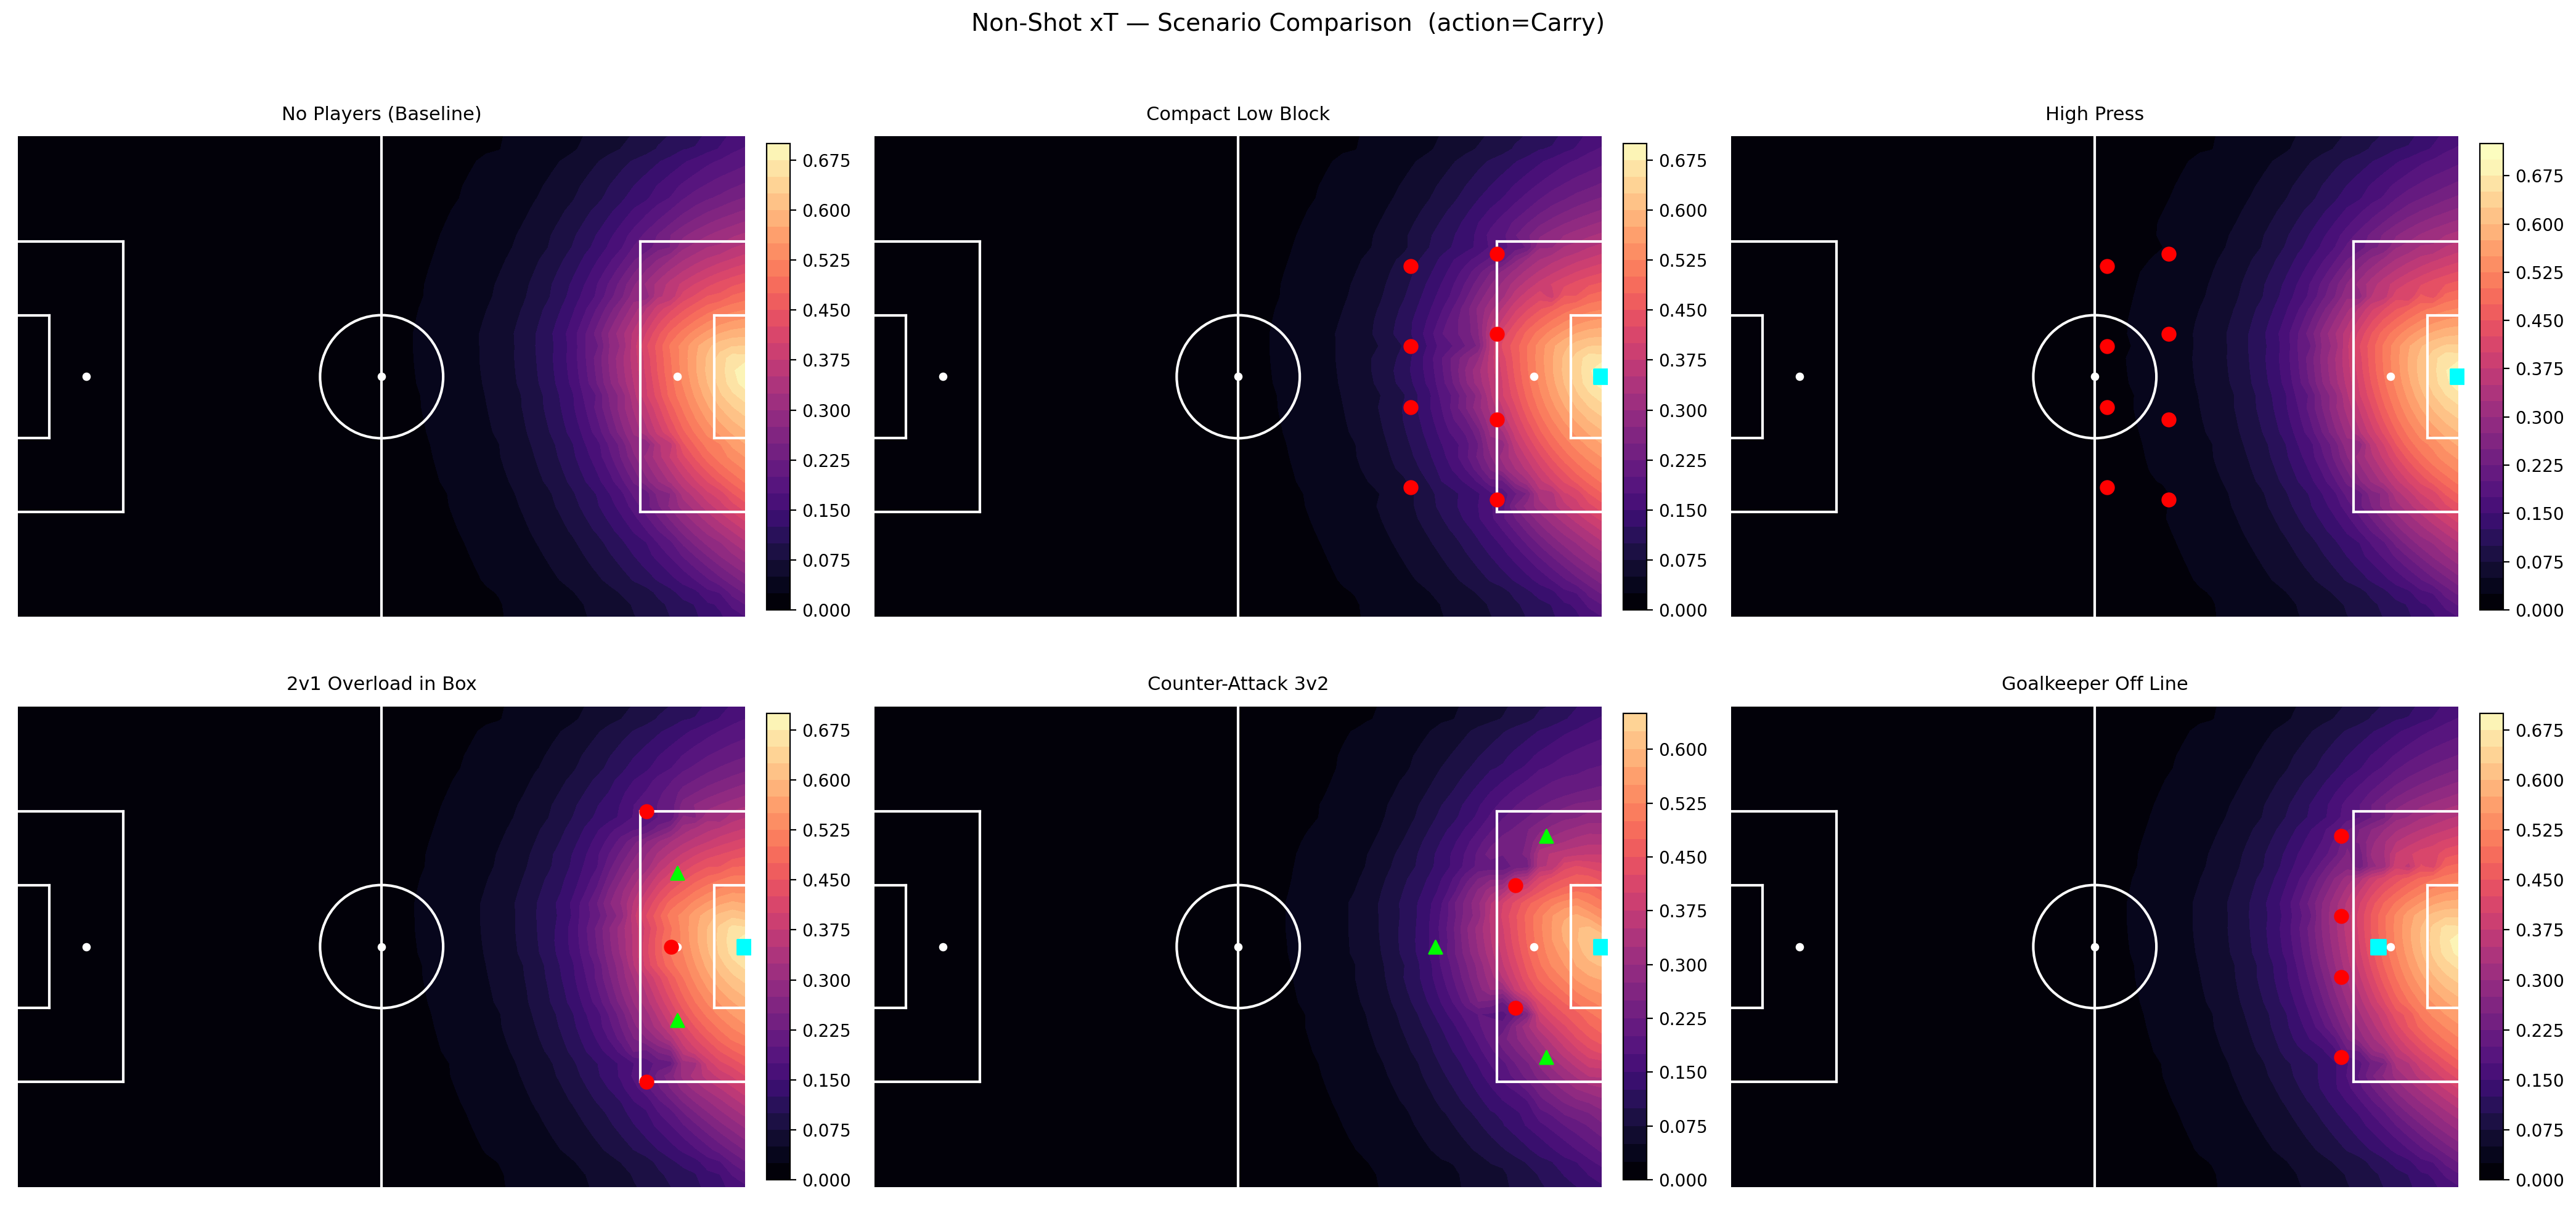
\includegraphics[width=0.8\textwidth]{../visualisations/xt_scenarios_carry_v2.png}
    \caption{Version 2 scenario comparison, Carry action type. End position is inferred as 8 yards toward goal from each cell. Surfaces are near-identical across formations, confirming the CNN's inability to distinguish between defensive configurations of equal density.}
    \label{fig:v2_scenarios_carry}
\end{figure}

\begin{figure}[h]
    \centering
    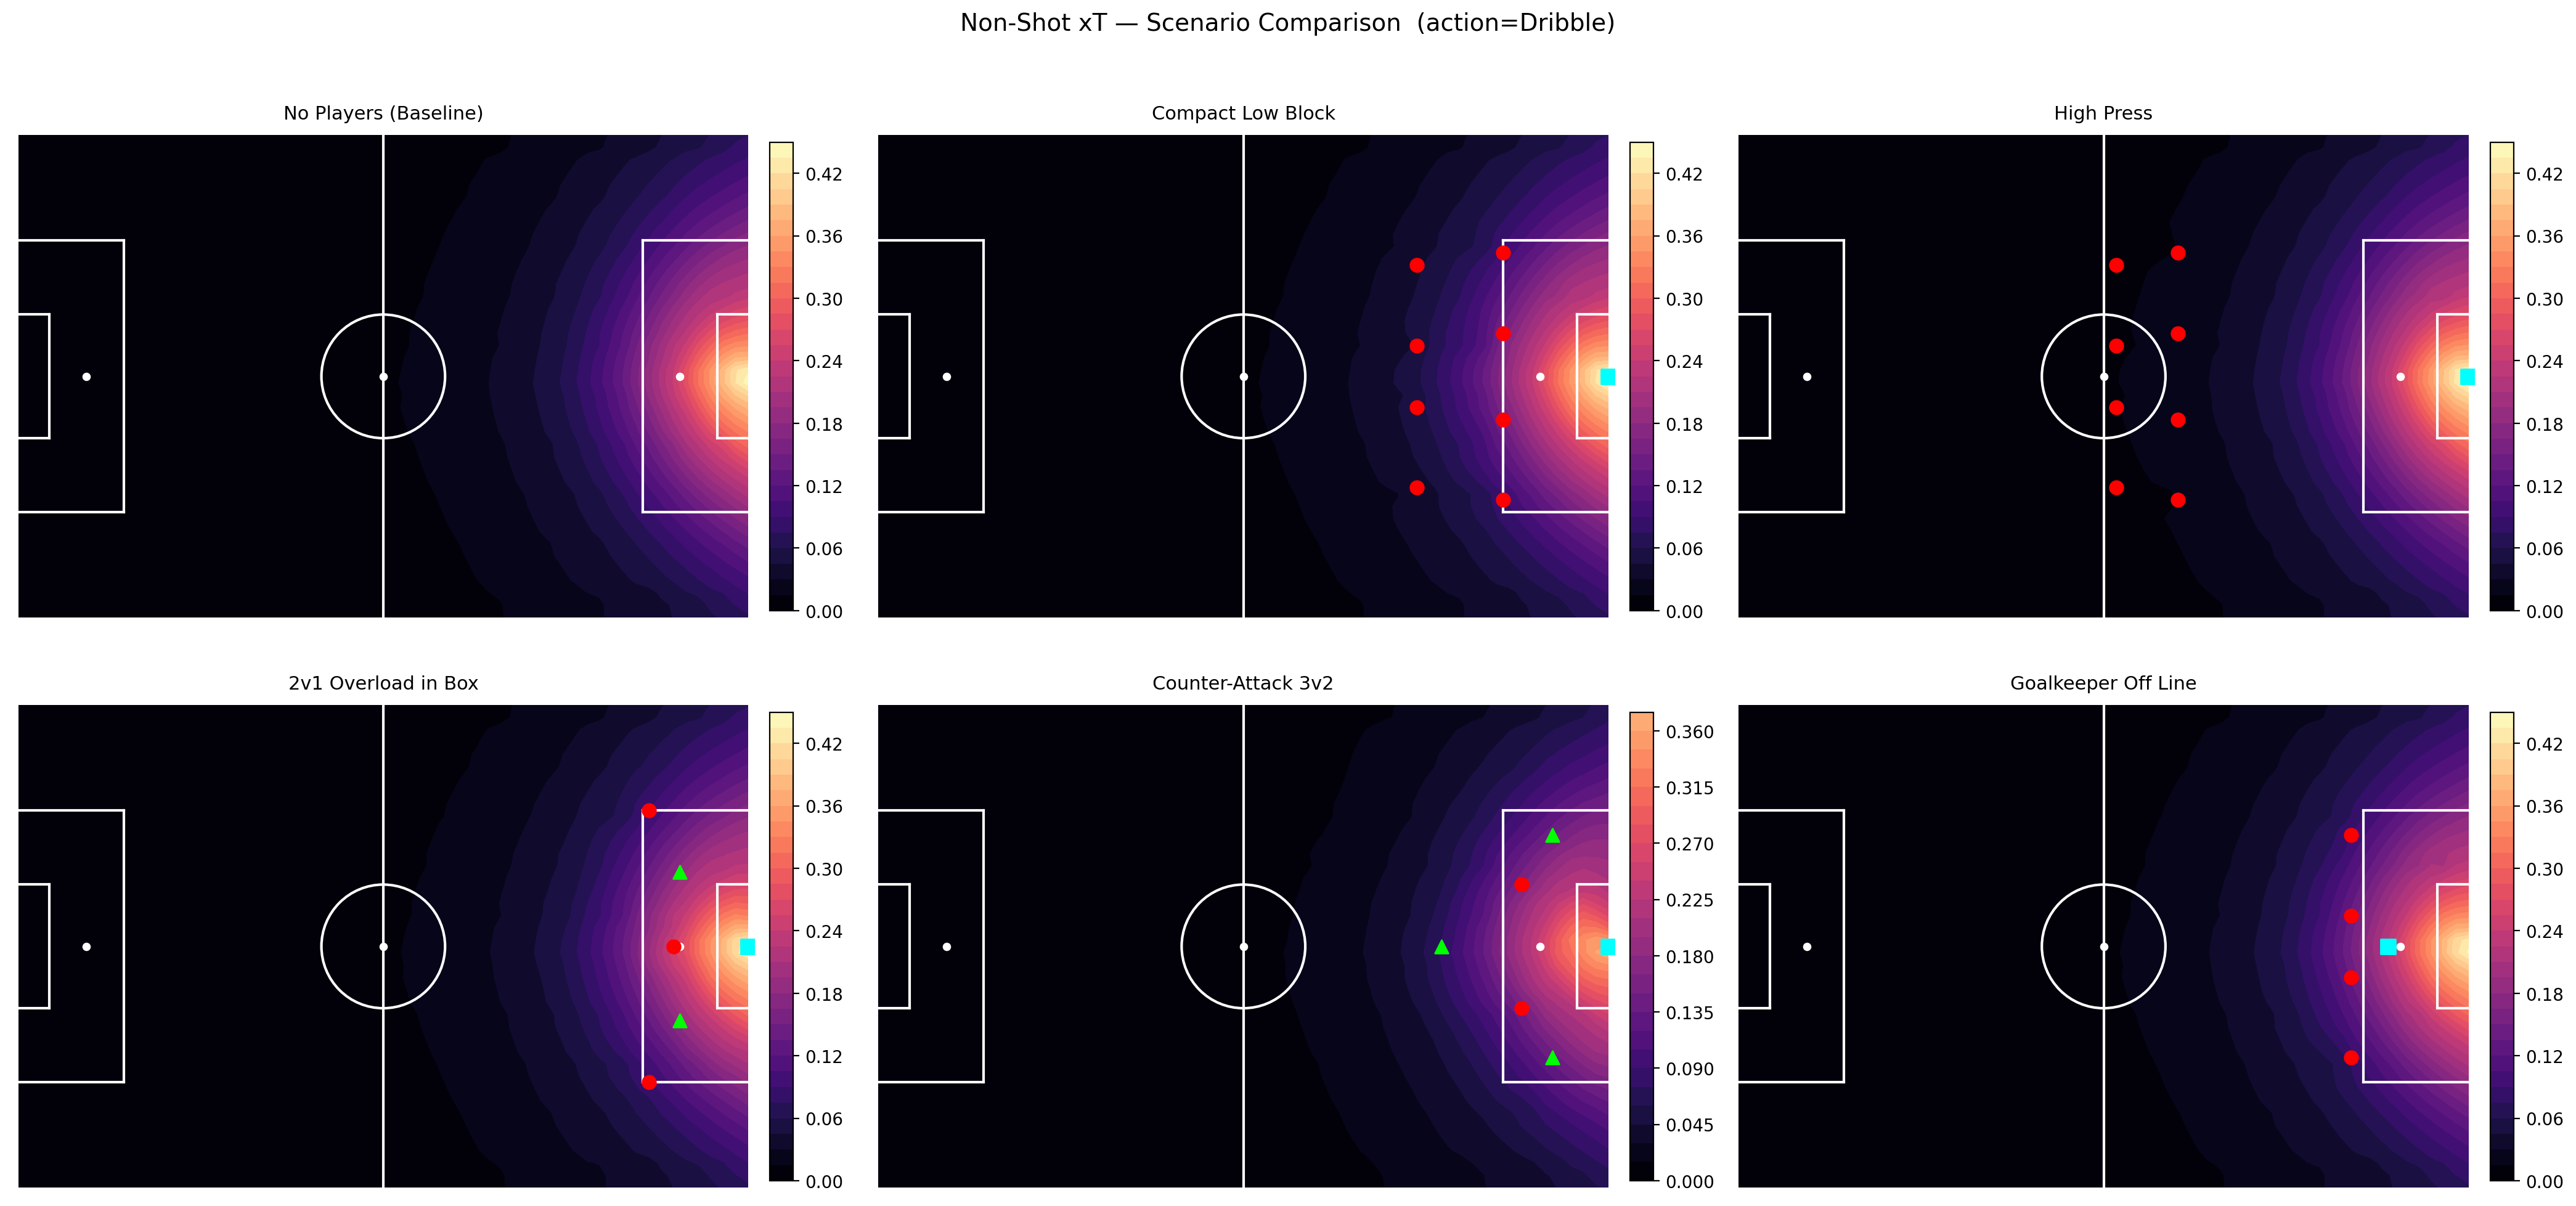
\includegraphics[width=0.8\textwidth]{../visualisations/xt_scenarios_dribble_v2.png}
    \caption{Version 2 scenario comparison, Dribble action type. End position is the ball position itself (no advancement), matching the StatsBomb training convention. Surfaces remain near-identical across formations, consistent with Version 2's structural inability to reason about individual player positions.}
    \label{fig:v2_scenarios_dribble}
\end{figure}

\section{Version 3: Transformer}

\begin{figure}[h]
\centering
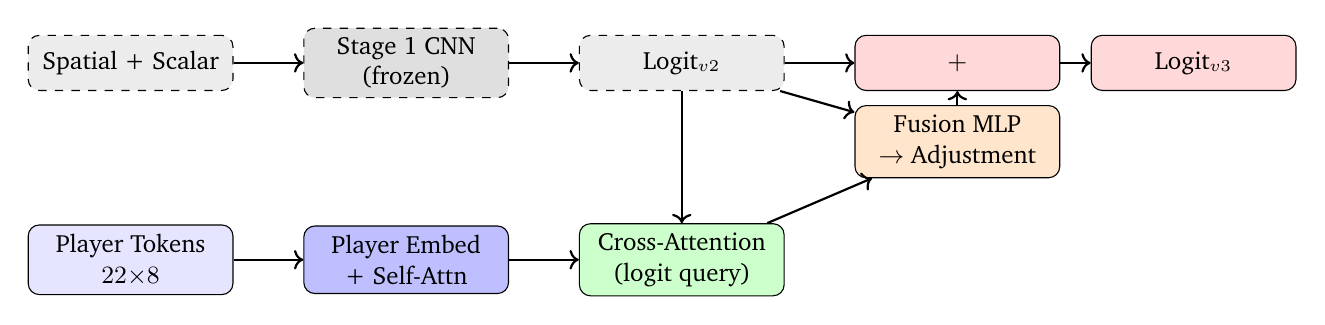
\begin{tikzpicture}[
    box/.style={draw, rounded corners, minimum width=2.6cm, minimum height=0.7cm, align=center, font=\small},
    frozen/.style={draw, rounded corners, minimum width=2.6cm, minimum height=0.7cm, align=center, font=\small, dashed},
    arr/.style={->, thick}
]
\node[frozen, fill=gray!15]  (sp)     at (0, 4)    {Spatial + Scalar};
\node[frozen, fill=gray!25]  (v2)     at (3.5, 4)  {Stage 1 CNN\\(frozen)};
\node[frozen, fill=gray!15]  (logit1) at (7, 4)    {Logit$_{v2}$};

\node[box, fill=blue!10]  (ptok)   at (0, 1.5)  {Player Tokens\\$22{\times}8$};
\node[box, fill=blue!25]  (embed)  at (3.5, 1.5){Player Embed\\+ Self-Attn};
\node[box, fill=green!20] (cross)  at (7, 1.5)  {Cross-Attention\\(logit query)};
\node[box, fill=orange!20](fusion) at (10.5,3)  {Fusion MLP\\$\to$ Adjustment};

\node[box, fill=red!15]   (add)    at (10.5, 4) {$+$};
\node[box, fill=red!15]   (out)    at (13.5, 4) {Logit$_{v3}$};

\draw[arr] (sp)     -- (v2);
\draw[arr] (v2)     -- (logit1);
\draw[arr] (logit1) -- (add);
\draw[arr] (ptok)   -- (embed);
\draw[arr] (embed)  -- (cross);
\draw[arr] (logit1) -- (cross);
\draw[arr] (cross)  -- (fusion);
\draw[arr] (logit1) -- (fusion);
\draw[arr] (fusion) -- (add);
\draw[arr] (add)    -- (out);
\end{tikzpicture}
\caption{Version 3 two-stage architecture. The frozen Stage 1 CNN (dashed) produces a baseline logit. Stage 2 encodes player tokens through self-attention (left branch); the Stage 1 logit is projected to a query vector that attends over the player context via cross-attention. The attended context and the Stage 1 logit are fused by the MLP to produce a scalar adjustment, which is added to the Stage 1 logit.}
\label{fig:v3arch}
\end{figure}

\begin{figure}[h]
    \centering
    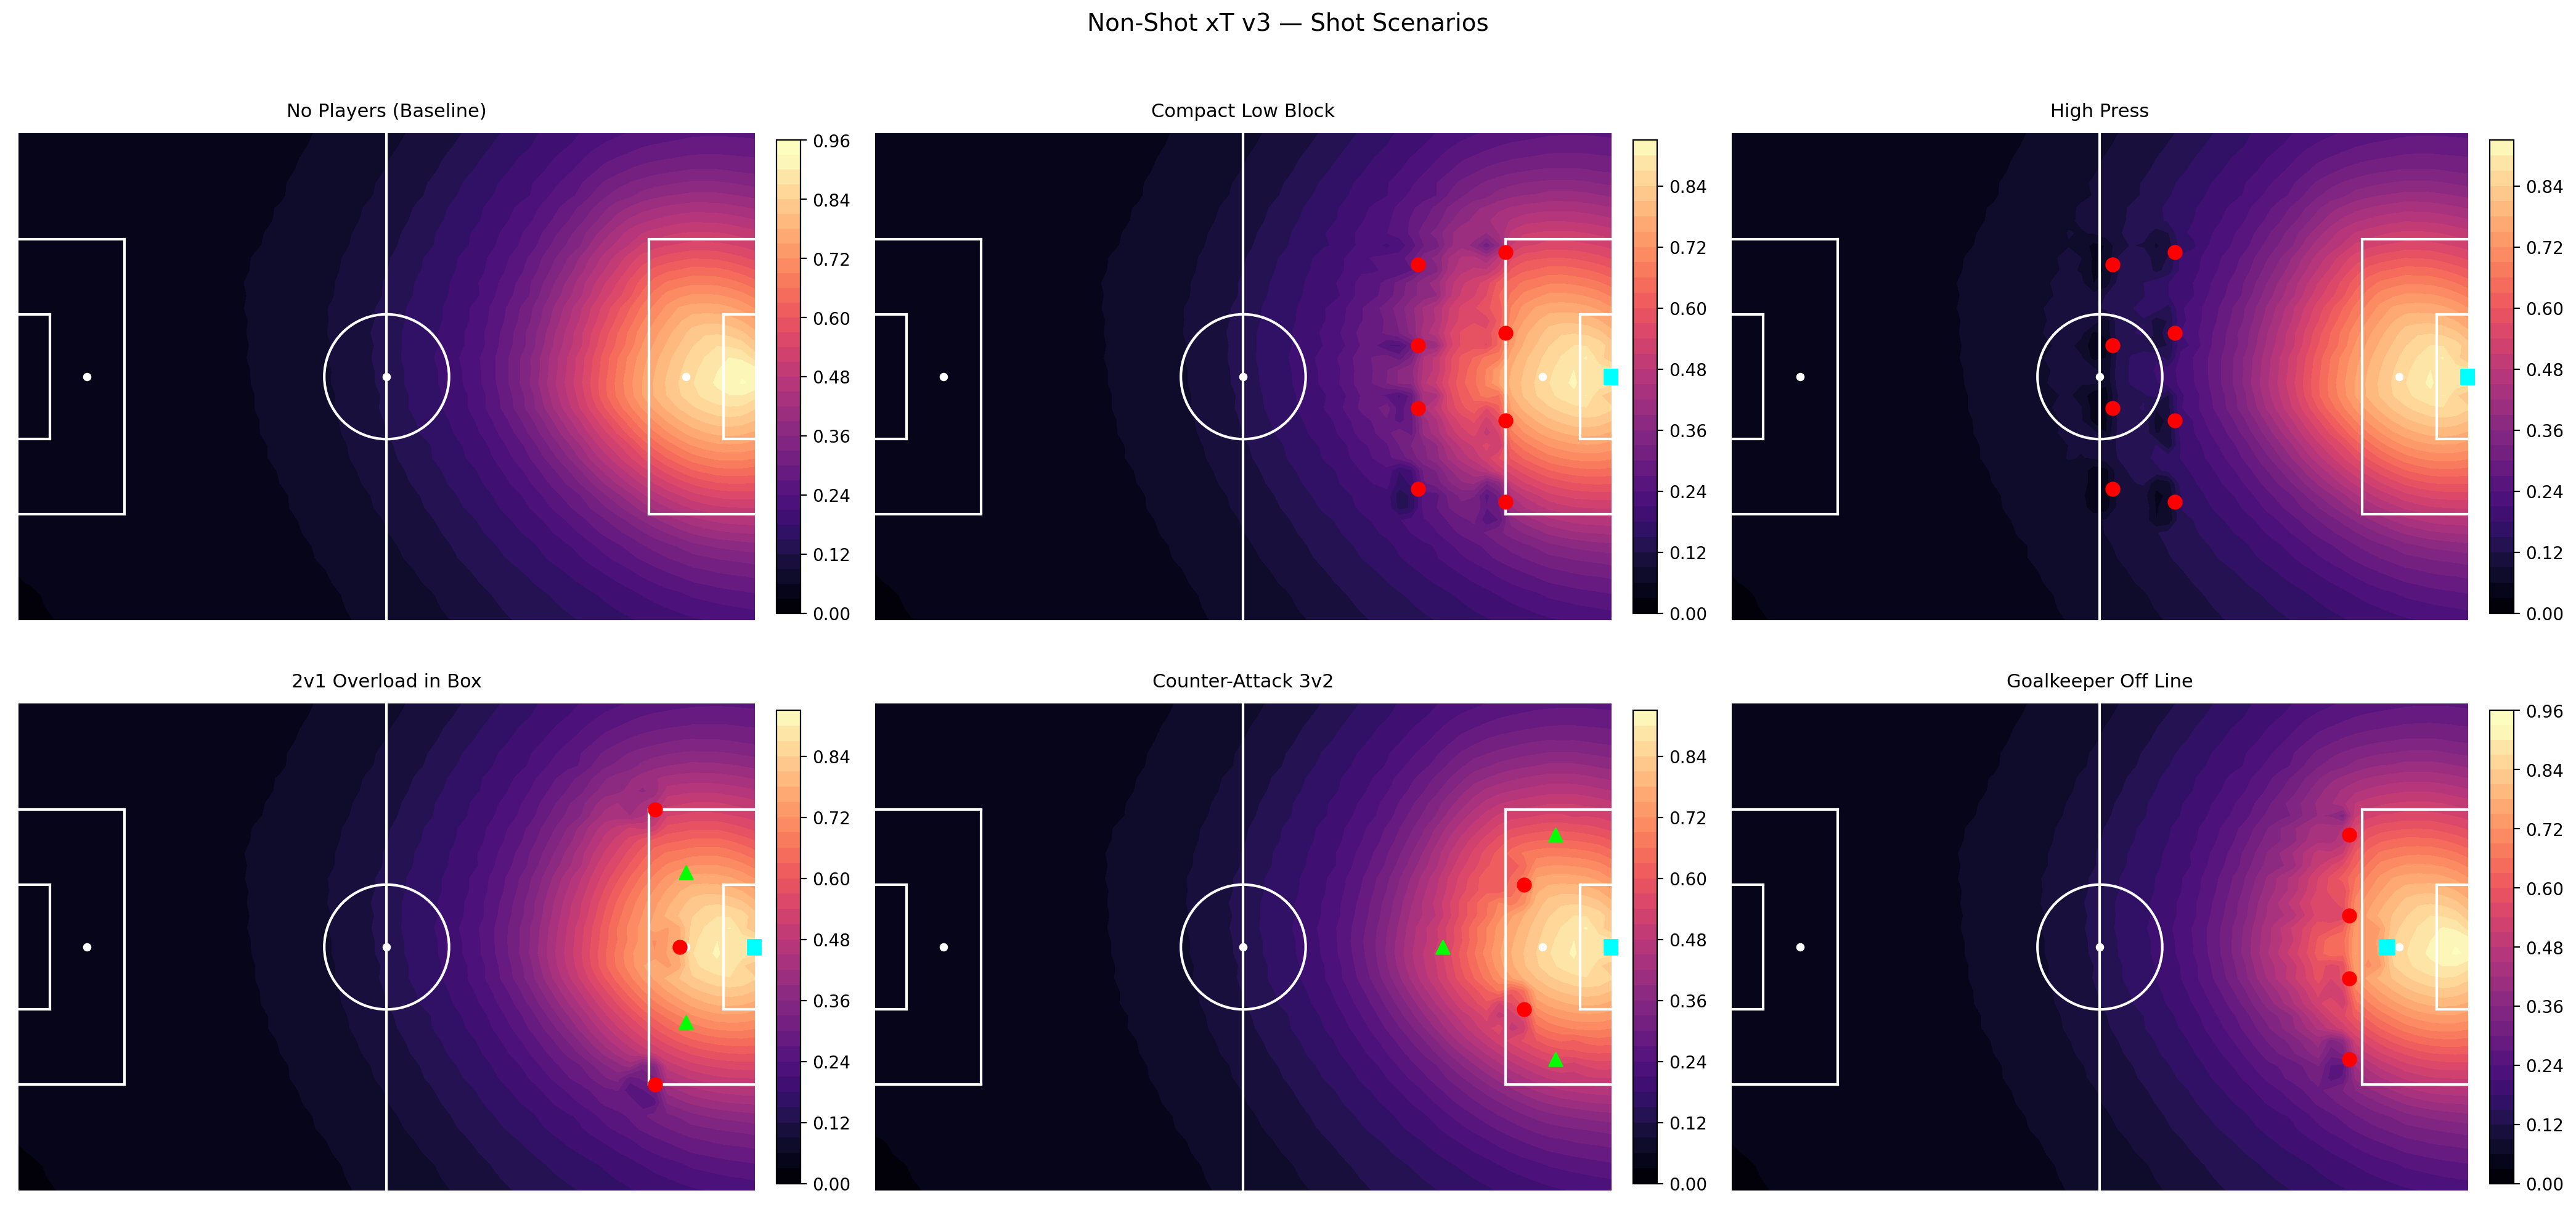
\includegraphics[width=0.8\textwidth]{../visualisations/xt_scenarios_shot_v3.png}
    \caption{Scenario comparison for Version 3, Shot action type. The first panel (no players) serves as the positional baseline. Different defensive formations produce visibly distinct threat landscapes --- a qualitative contrast to the near-identical Version 2 panels. These are illustrative inputs, not held-out measurements; the ablation (Section~\ref{sec:v3_ablation}) quantifies the player-token contribution on held-out data.}
    \label{fig:v3_scenarios}
\end{figure}

\label{sec:v3_scenarios_appendix}
The following figures show Version 3 scenario grids for Pass, Carry, and Dribble. The Pass black-panel convention (zero xT when no outfield teammates are present) is the same as for Version 2 above. For scenarios with teammates, Version 3 evaluates each teammate's position as a pass target and shows the maximum xT, using the per-player token representation of the Transformer.

\begin{figure}[h]
    \centering
    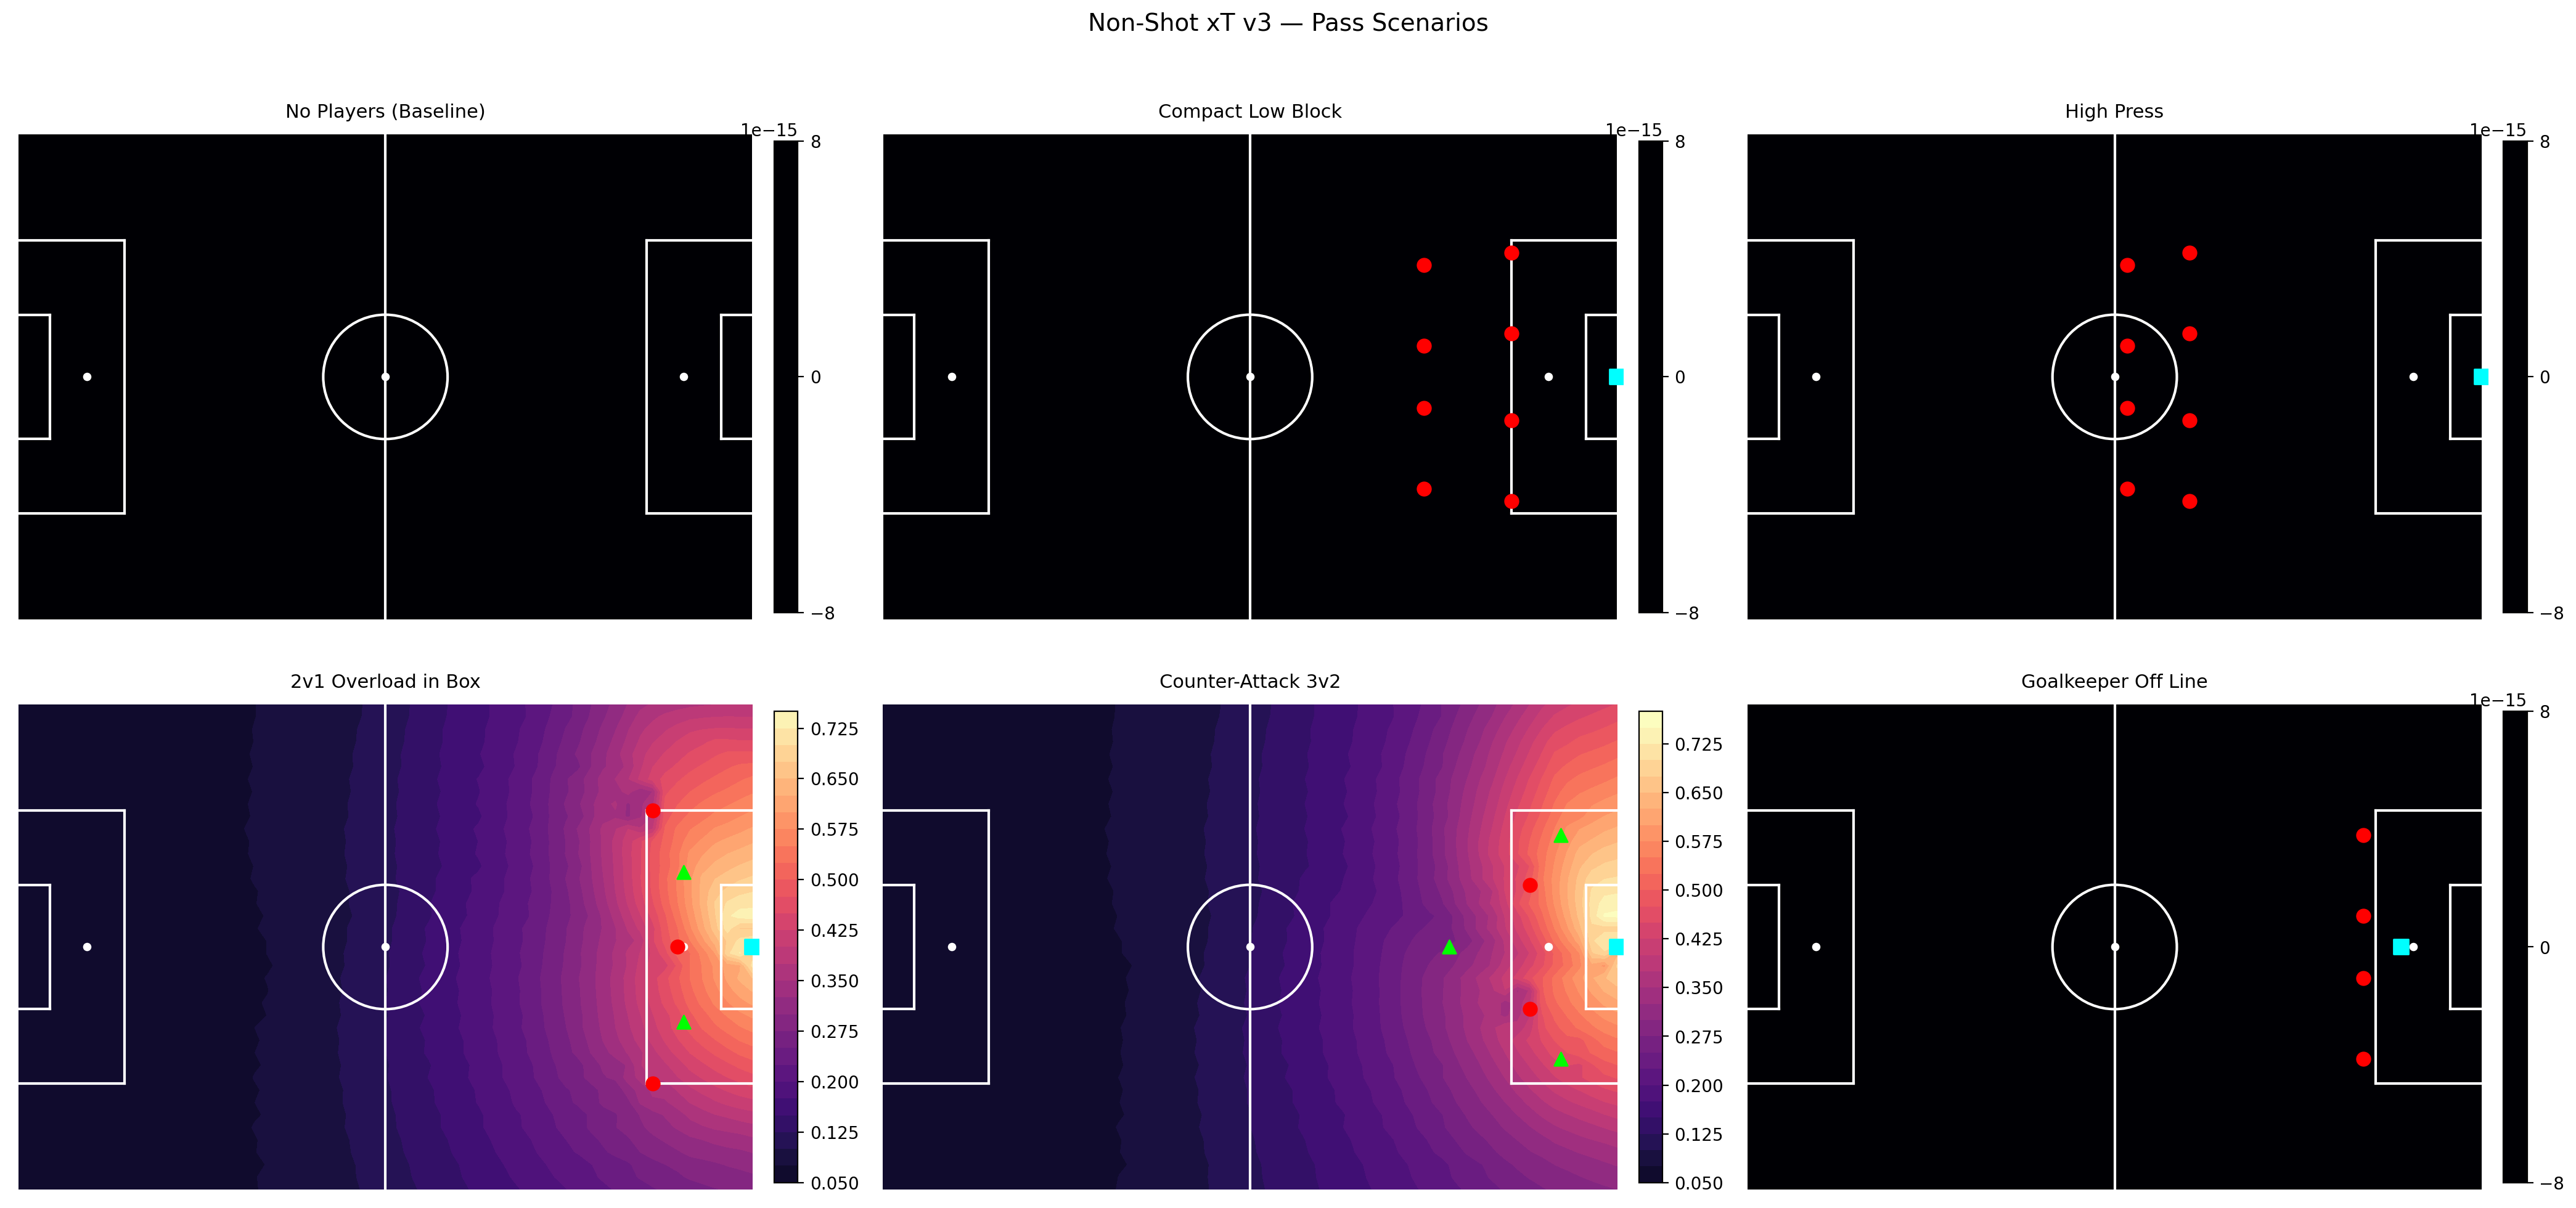
\includegraphics[width=0.8\textwidth]{../visualisations/xt_scenarios_pass_v3.png}
    \caption{Version 3 scenario comparison, Pass action type. Panels without outfield teammates are black by design. The 2v1 Overload and Counter-Attack panels show elevated Pass threat where the Transformer recognises the positioning of teammates relative to defenders, producing non-uniform threat surfaces that differ from the Version 2 equivalents.}
    \label{fig:v3_scenarios_pass}
\end{figure}

\begin{figure}[h]
    \centering
    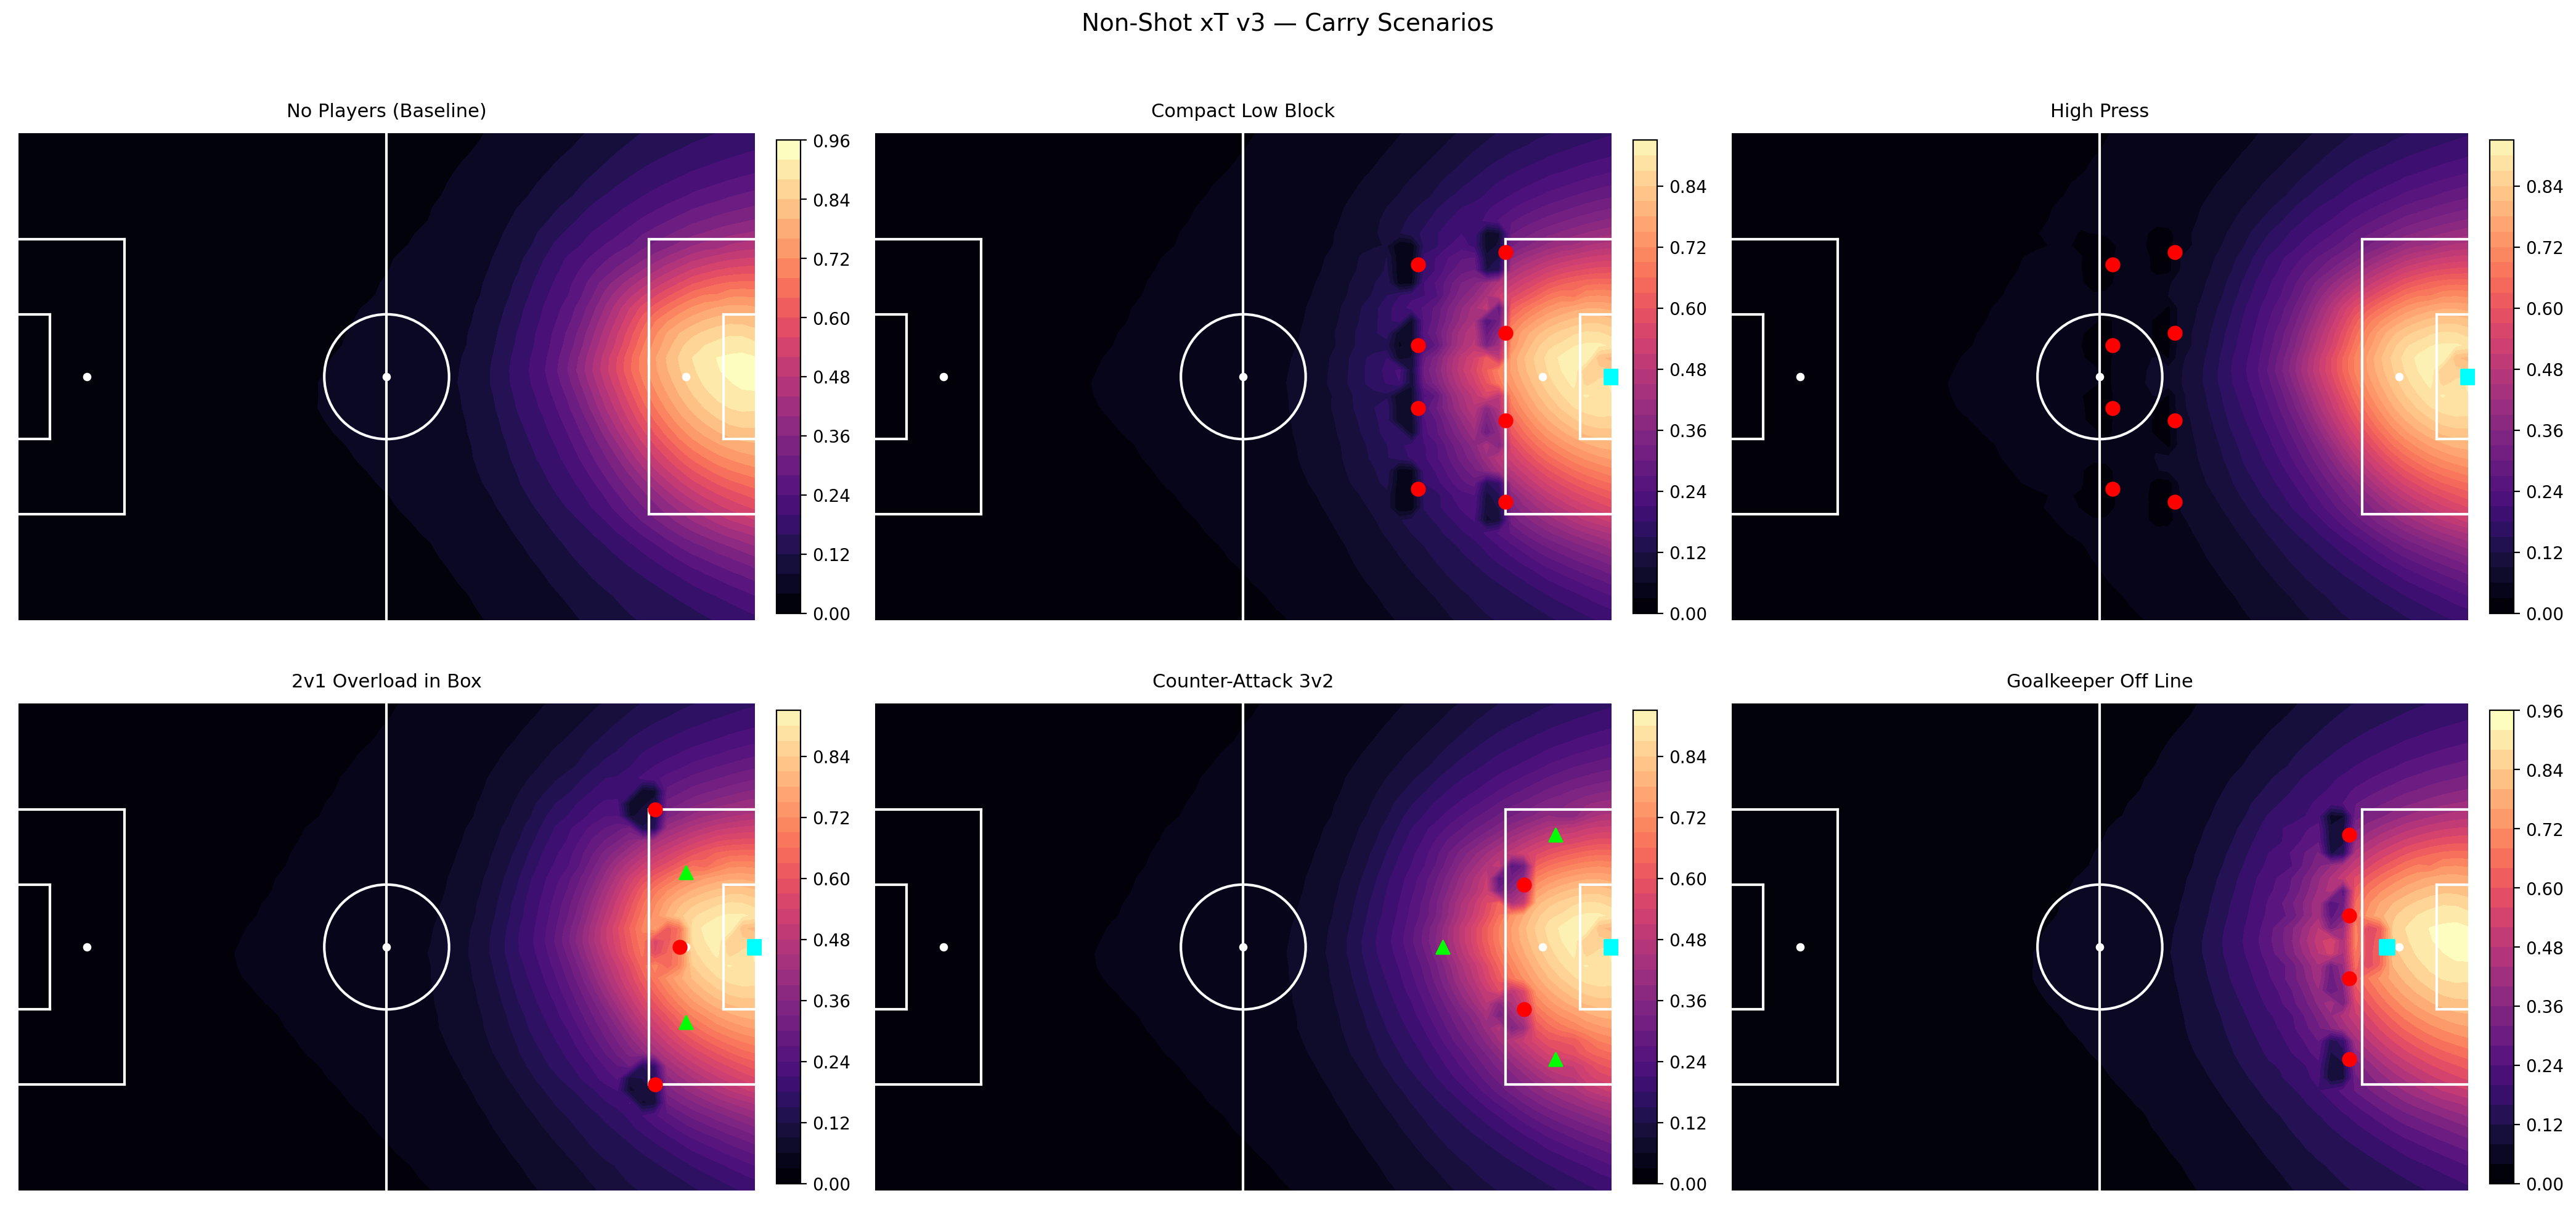
\includegraphics[width=0.8\textwidth]{../visualisations/xt_scenarios_carry_v3.png}
    \caption{Version 3 scenario comparison, Carry action type. End position is inferred as 8 yards toward goal from each cell. Unlike Version 2, the Transformer produces formation-sensitive surfaces: the Compact Low Block and High Press scenarios yield visibly different patterns, reflecting the model's ability to reason about individual defender positions relative to the carry path.}
    \label{fig:v3_scenarios_carry}
\end{figure}

\begin{figure}[h]
    \centering
    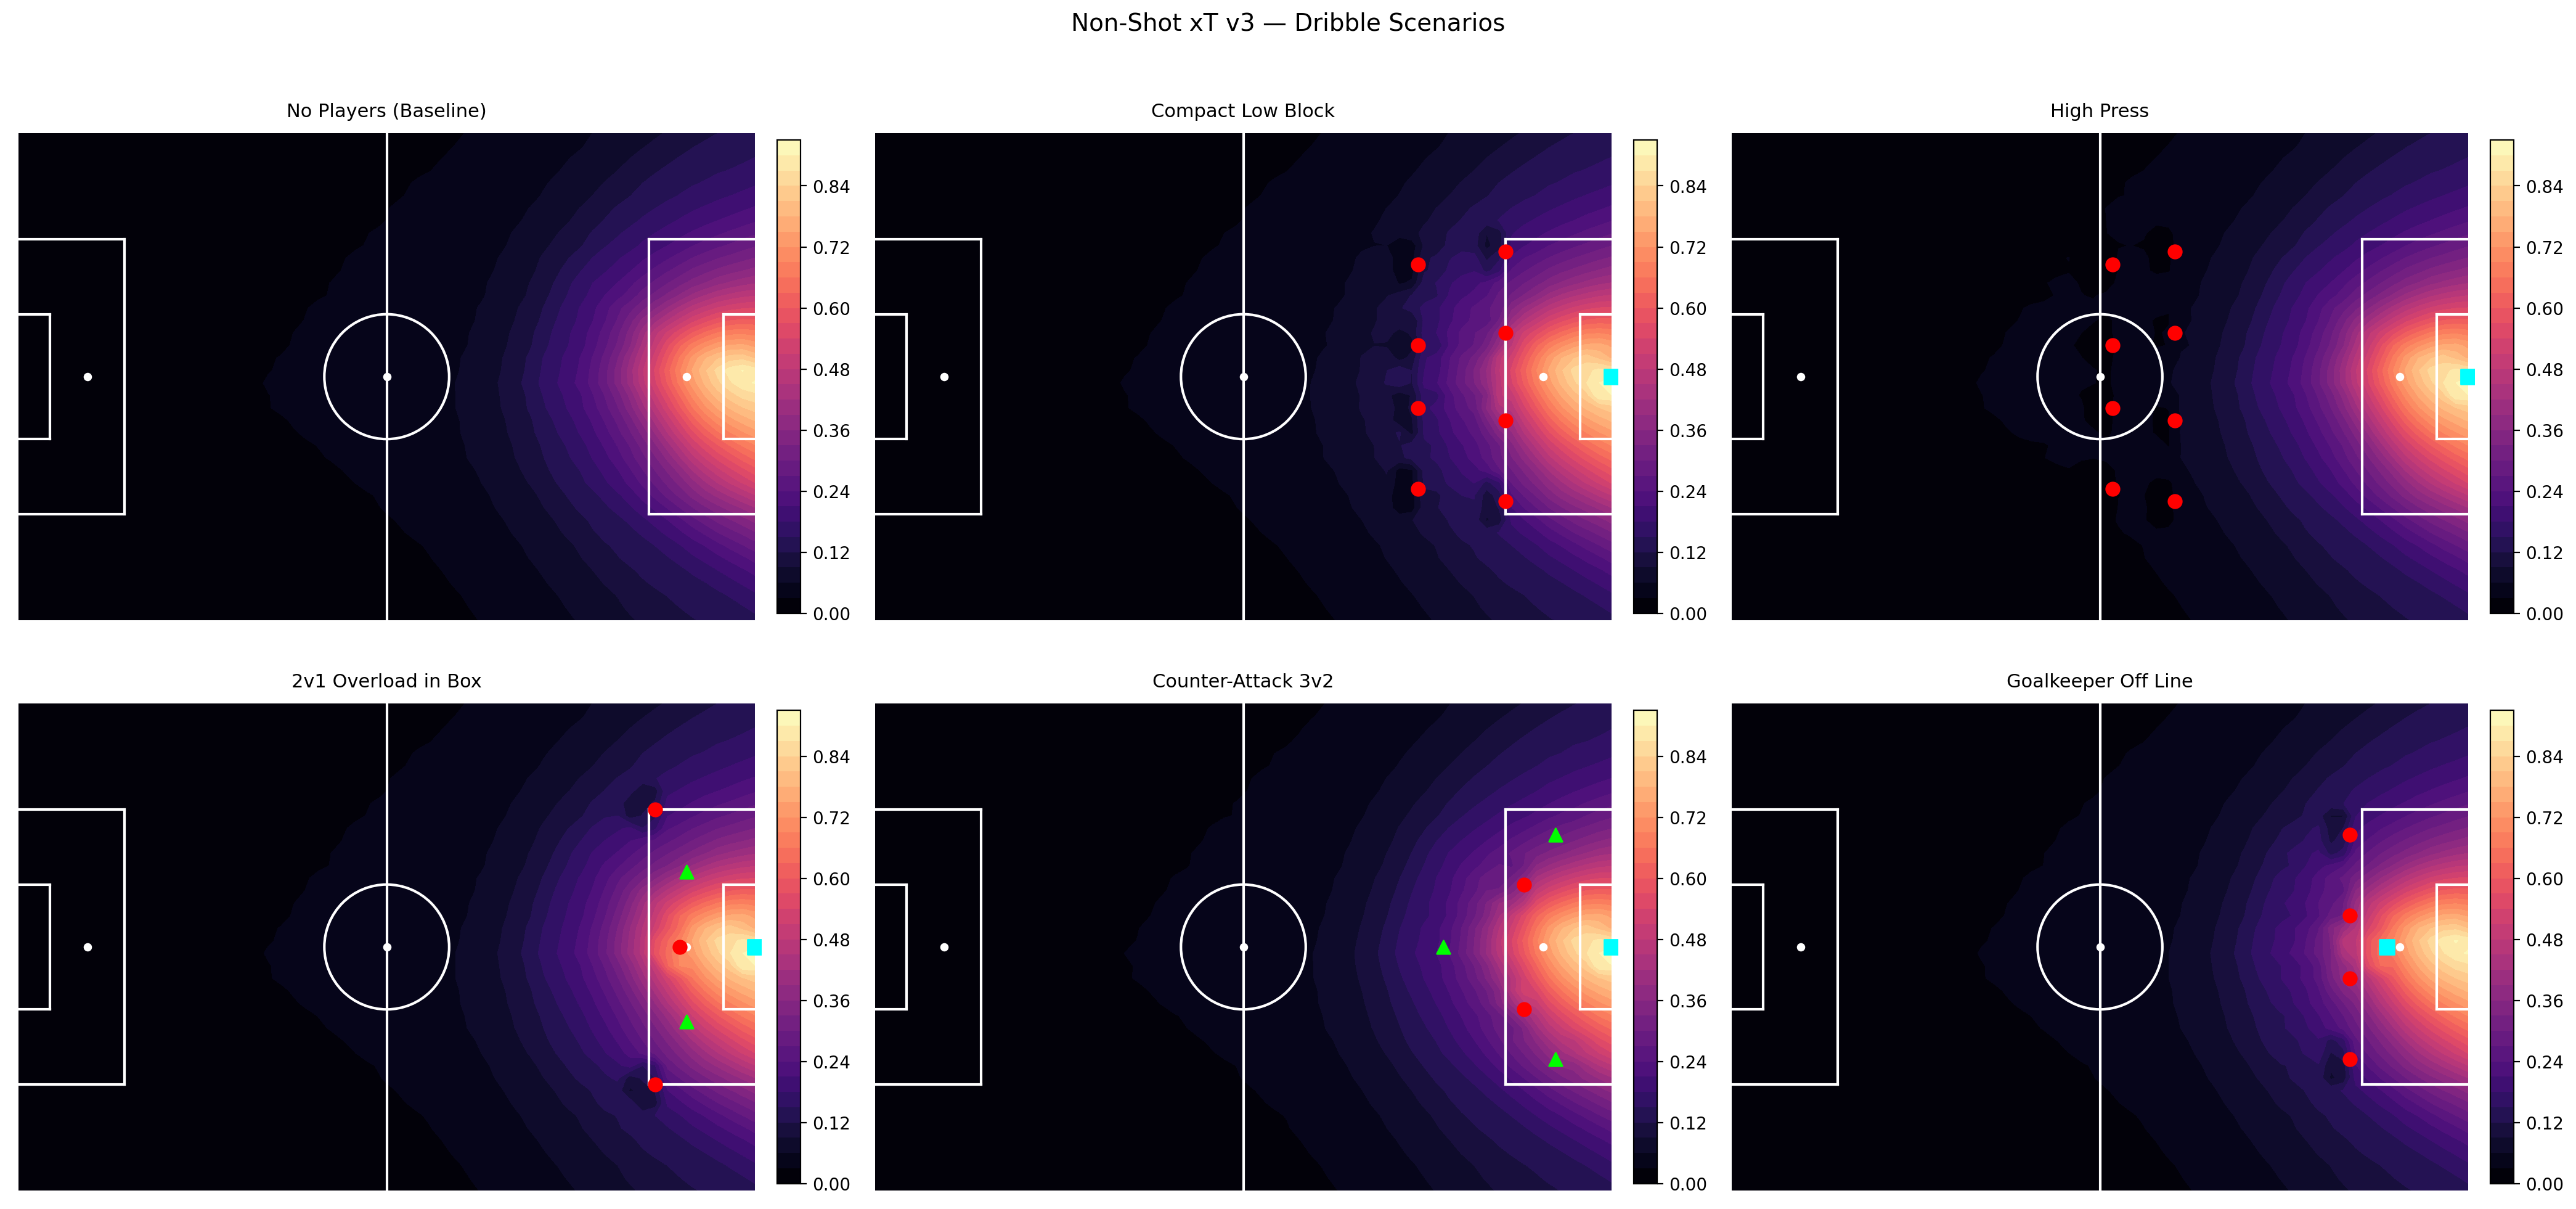
\includegraphics[width=0.8\textwidth]{../visualisations/xt_scenarios_dribble_v3.png}
    \caption{Version 3 scenario comparison, Dribble action type. End position is the ball position itself (no advancement). The Transformer's player-token representation allows it to modulate threat based on how many defenders are immediately goalside of the ball carrier, producing formation-sensitive outputs absent from Version 2.}
    \label{fig:v3_scenarios_dribble}
\end{figure}

\clearpage

\section{Interactive Frontend}

\begin{figure}[h]
    \centering
    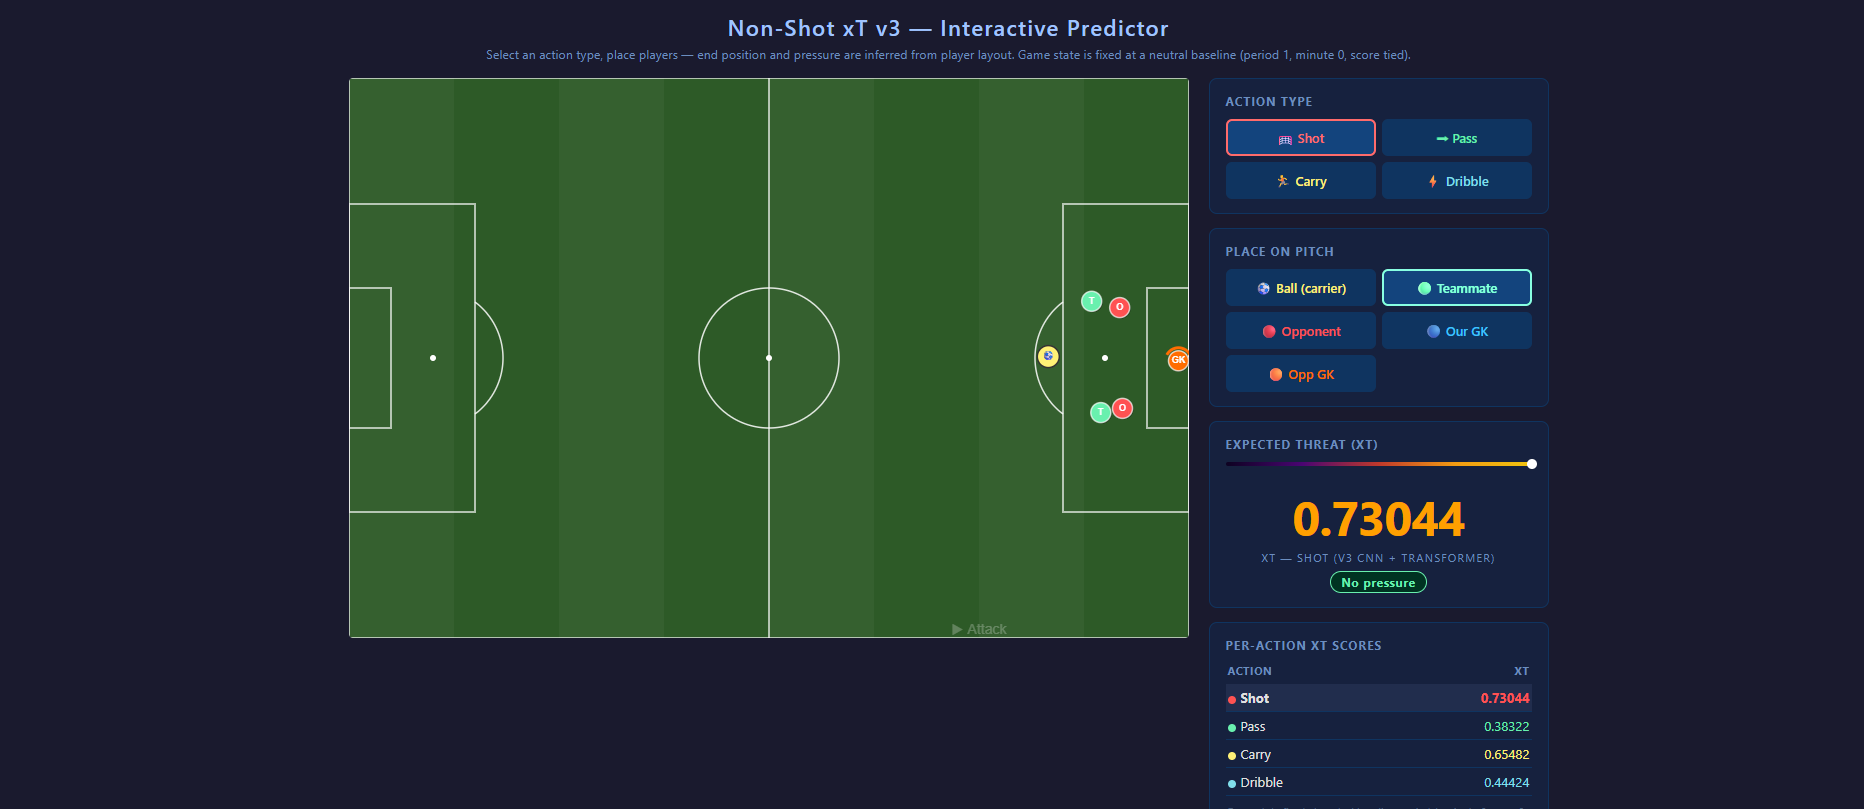
\includegraphics[width=\textwidth]{../visualisations/frontend_screenshot.png}
    \caption{Interactive xT web frontend: ball carrier placed near the edge of the penalty area with teammates and opponents in the box. The Shot action type is selected; the model returns an xT of 0.73044 for a shot from this position with this player layout. The per-action table alongside shows all four action scores simultaneously. Game state is fixed at a neutral baseline (period 1, minute 0, score tied).}
    \label{fig:frontend}
\end{figure}


\bibliography{bibliography}

\end{document}
